\documentclass[10pt,adobefonts,fancyhdr,hyperref,UTF8]{ctexbook}

\usepackage{multirow}
% for \soul 删除线
\usepackage{ulem}
% 表头斜线
\usepackage{diagbox}

\makeatletter
\usepackage[centering,paperwidth=180mm,paperheight=230mm,%
body={390pt,530pt},marginparsep=10pt,marginpar=50pt]{geometry}
\usepackage{color}
\usepackage{enumitem}
\usepackage{fancyvrb}
\usepackage[bottom,perpage,symbol*]{footmisc}
\usepackage{graphicx}
\usepackage[hidelinks]{hyperref}
\usepackage{makeidx}
\usepackage[toc]{multitoc}
\usepackage{pifont}
\usepackage{underscore}
\usepackage{amsmath}

\DefineFNsymbols*{chinese}{{\ding{172}}{\ding{173}}{\ding{174}}{\ding{175}}%
{\ding{176}}{\ding{177}}{\ding{178}}{\ding{179}}{\ding{180}}{\ding{181}}}
\setfnsymbol{chinese}

\hypersetup{bookmarksnumbered=true,bookmarksdepth=2}

\CTEXsetup[number={\thechapter}]{chapter}
\CTEXsetup[format+={\raggedleft}]{chapter}
\CTEXsetup[beforeskip={10pt}]{chapter}
\CTEXsetup[afterskip={30pt}]{chapter}
\def\CTEX@chapter@aftername{\par} % \CTEXsetup[aftername={\par}]{chapter}
\CTEXsetup[format+={\raggedright}]{section}
\CTEXsetup[beforeskip={-3.0ex plus -1ex minus -.2ex}]{section}
\CTEXsetup[afterskip={2.3ex plus .2ex minus 0.2ex}]{section}

\renewcommand \thefigure{\thechapter-\arabic{figure}}
\renewcommand \thetable{\thechapter-\arabic{table}}

\newcommand\figcaption[1]{\def\@captype{figure}\caption{#1}}
\newcommand\tabcaption[1]{\def\@captype{table}\caption{#1}}

\long\def\@caption#1[#2]#3{%
  \addcontentsline{\csname ext@#1\endcsname}{#1}%
    {\protect\numberline{\csname fnum@#1\endcsname}{ \ignorespaces #2}}% change "the" to "fnum@"
    \normalsize
    \@makecaption{\csname fnum@#1\endcsname}{\ignorespaces #3}}

\long\def\@makecaption#1#2{%
  \vskip\abovecaptionskip
  \sbox\@tempboxa{#1\quad#2}%
  \ifdim \wd\@tempboxa >\hsize
    #1\quad#2\par
  \else
    \global \@minipagefalse
    \hb@xt@\hsize{\hfil\box\@tempboxa\hfil}%
  \fi
  \vskip\belowcaptionskip}

\setlength\abovecaptionskip{0pt}
  
%\setmainfont{Times New Roman}
\setmainfont{Linux Libertine O}
%\setmainfont{TeX Gyre Pagella}
\newfontfamily\urlfont{PT Sans Narrow}
%\setmonofont[AutoFakeBold=1.6,AutoFakeSlant=0.17,Mapping=tex-text-tt]{Inconsolata}
\setCJKfamilyfont{zhyou}{YouYuan}

\newcommand{\fn}[1]{\texttt{#1}}
\newcommand{\sfn}[1]{\texttt{\small #1}}
\newcommand{\kw}[1]{\textsf{#1}}
\newcommand{\myurl}[1]{{\urlfont #1}}
\newcommand{\mpar}[1]{\marginpar[\hfill\kaishu #1]{\kaishu #1}}
\newcommand{\mn}[1]{\texttt{\bs #1}}
\renewcommand{\today}{\the\year-\the\month-\the\day}
\newcommand\bs{\textbackslash}
\newcommand{\code}[1]{\small{\fontspec{Latin Modern Mono} #1}}

\newcommand\begindot{\begin{itemize}
[itemsep=2pt plus 2pt minus 2pt,%
topsep=3pt plus 2pt minus 2pt,%
parsep=0pt plus 2pt minus 2pt]}
\newcommand\myenddot{\end{itemize}}

\newcommand\beginnum{\begin{enumerate}
[itemsep=2pt plus 2pt minus 2pt,%
topsep=3pt plus 2pt minus 2pt,%
parsep=0pt plus 2pt minus 2pt]}
\newcommand\myendnum{\end{enumerate}}

\DefineVerbatimEnvironment%
  {Code}{Verbatim}
  {fontsize=\small,baselinestretch=0.9,xleftmargin=3mm}

\raggedbottom
%\setlength{\parskip}{1ex plus .5ex minus .5ex}

\def\FV@SetLineWidth{%
  \if@FV@ResetMargins\else
    \advance\leftmargin\@totalleftmargin
  \fi
  \advance\leftmargin\FV@XLeftMargin\relax
  \advance\rightmargin\FV@XRightMargin\relax
  \linewidth\hsize
  %\advance\linewidth-\leftmargin
  %\advance\linewidth-\rightmargin
  \hfuzz\FancyVerbHFuzz\relax}


\def\FV@SingleFrameLine#1{%
%% DG/SR modification end
  \hbox to\z@{%
    %\kern\leftmargin
%% DG/SR modification begin - Jun. 22, 1998
    \ifnum#1=\z@
      \let\FV@Label\FV@LabelBegin
    \else
      \let\FV@Label\FV@LabelEnd
    \fi
    \ifx\FV@Label\relax
%% DG/SR modification end
      \FancyVerbRuleColor{\vrule \@width\linewidth \@height\FV@FrameRule}%
%% DG/SR modification begin - Jun. 22, 1998
    \else
      \ifnum#1=\z@
        \setbox\z@\hbox{\strut\enspace\urlfont\FV@LabelBegin\strut}%
      \else
        \setbox\z@\hbox{\strut\enspace\urlfont\FV@LabelEnd\strut}%
      \fi
      \@tempdimb=\dp\z@
      \advance\@tempdimb -.5\ht\z@
      \@tempdimc=\linewidth
      \advance\@tempdimc -\wd\z@
      %\divide\@tempdimc\tw@
      \ifnum#1=\z@              % Top line
        \ifx\FV@LabelPositionTopLine\relax
          \FancyVerbRuleColor{\vrule \@width\linewidth \@height\FV@FrameRule}%
        \else
          \FV@FrameLineWithLabel
        \fi
      \else                     % Bottom line
        \ifx\FV@LabelPositionBottomLine\relax
          \FancyVerbRuleColor{\vrule \@width\linewidth \@height\FV@FrameRule}%
        \else
          \FV@FrameLineWithLabel
        \fi
      \fi
    \fi
%% DG/SR modification end
    \hss}}


%% DG/SR modification begin - May. 19, 1998
\def\FV@FrameLineWithLabel{%
  \ht\z@\@tempdimb\dp\z@\@tempdimb%
  \FancyVerbRuleColor{%
    \raise 0.5ex\hbox{\vrule \@width\@tempdimc \@height\FV@FrameRule}%
    \raise\@tempdimb\box\z@}}
%% DG/SR modification end


\def\FV@EndListFrame@Lines{%
  \begingroup
    %\vskip 0.5ex
    \baselineskip\z@skip
    \kern\FV@FrameSep\relax
%% DG/SR modification begin - May. 19, 1998
%%    \FV@SingleFrameLine
    \FV@SingleFrameLine{\@ne}%
%% DG/SR modification end
  \endgroup}

\newskip\mytopsep
\setlength{\mytopsep}{4pt plus 2pt minus 3pt}

\def\FV@ListVSpace{%
  \@topsepadd\mytopsep
  \if@noparlist\advance\@topsepadd\partopsep\fi
  \if@inlabel
    \vskip\parskip
  \else
    \if@nobreak
      \vskip\parskip
      \clubpenalty\@M
    \else
      \addpenalty\@beginparpenalty
      \@topsep\@topsepadd
      \advance\@topsep\parskip
      \addvspace\@topsep
    \fi
  \fi
  %\showthe \@topsepadd
  %\showthe \topsep
  %\showthe \partopsep
  %\showthe \parskip
  \global\@nobreakfalse
  \global\@inlabelfalse
  \global\@minipagefalse
  \global\@newlistfalse}

\def\FV@EndList{%
  \FV@ListProcessLastLine
  \FV@EndListFrame
  %\showthe \@topsepadd
  \@endparenv
  \endgroup
  \@endpetrue}

\def\theFancyVerbLine{\sffamily\scriptsize\arabic{FancyVerbLine}}

\DefineVerbatimEnvironment%
  {Codex}{Verbatim}
  {fontsize=\small,baselinestretch=0.9,xleftmargin=3mm,%
  frame=lines,labelposition=all,framesep=5pt}

\DefineVerbatimEnvironment%
  {Code}{Verbatim}
  {fontsize=\small,baselinestretch=0.9,xleftmargin=3mm}

\makeindex

\makeatother

\begin{document}
\sloppy
\newcommand\BookTitle{LeetCode题解}
\pagestyle{fancy}
\fancyhf{}
\fancyhead[RE]{\normalfont\small\rmfamily\nouppercase{\leftmark}}
\fancyhead[LO]{\normalfont\small\rmfamily\nouppercase{\rightmark}}
\fancyhead[LE,RO]{\thepage}
%\fancyfoot[LE,LO]{\small\normalfont\youyuan\BookTitle}
%\fancyfoot[RE,RO]{\textsf{\small \color{blue} https://gitcafe.com/soulmachine/LeetCode}}

\makeatletter
\@openrightfalse
\makeatother

\frontmatter % 开始前言目录,页码用罗马数字

\thispagestyle{plain}
\begin{center}
  {\LARGE\textbf{\BookTitle}}

  \vspace{1em}
  {\large 灵魂机器 (soulmachine@gmail.com)}

  \vspace{1ex}
  \myurl{https://github.com/soulmachine/leetcode}
  
  \vspace{1ex}
  最后更新\, \today\, \thistime
  
  \vspace{1em}
  \textbf{\large 版权声明}
\end{center}
\noindent 本作品采用“Creative Commons 署名-非商业性使用-相同方式共享 3.0 Unported许可协议 
(cc by-nc-sa)”进行许可。
\texttt{\small http://creativecommons.org/licenses/by-nc-sa/3.0/}

\vspace{1em}
\subsubsection{内容简介}
本书的目标读者是准备去北美找工作的码农,也适用于在国内找工作的码农,以及刚接触ACM算法竞赛的新手。

本书包含了 LeetCode Online Judge(\myurl{http://leetcode.com/onlinejudge})所有题目的答案,
所有代码经过精心编写,编码规范良好,适合读者反复揣摩,模仿,甚至在纸上默写。

全书的代码,使用C++ 11的编写,并在 LeetCode Online Judge 上测试通过。本书中的代码规范,跟在公司中的工程规范略有不同,为了使代码短(方便迅速实现):

\begindot
\item 所有代码都是单一文件。这是因为一般OJ网站,提交代码的时候只有一个文本框,如果还是
按照标准做法,比如分为头文件.h和源代码.cpp,无法在网站上提交;

\item Shorter is better。能递归则一定不用栈;能用STL则一定不自己实现。

\item 不提倡防御式编程。不需要检查malloc()/new 返回的指针是否为nullptr;不需要检查内部函数入口参数的有效性。
\myenddot

本手册假定读者已经学过《数据结构》\footnote{《数据结构》,严蔚敏等著,清华大学出版社,
\myurl{http://book.douban.com/subject/2024655/}},
《算法》\footnote{《Algorithms》,Robert Sedgewick, Addison-Wesley Professional, \myurl{http://book.douban.com/subject/4854123/}}
这两门课,熟练掌握C++或Java。

\subsubsection{GitCafe地址}
本书是开源的,项目地址:\myurl{https://gitcafe.com/soulmachine/LeetCode}


\tableofcontents

\mainmatter % 开始正文,页码用阿拉伯数字

\graphicspath{{diagrams/}}

\chapter{线性表}
这类题目考察线性表的操作,例如,数组,单链表,双向链表等。


\section{数组} %%%%%%%%%%%%%%%%%%%%%%%%%%%%%%


\subsection{Remove Duplicates from Sorted Array}
\label{sec:remove-duplicates-from-sorted-array}


\subsubsection{描述}
Given a sorted array, remove the duplicates in place such that each element appear only once and return the new length.

Do not allocate extra space for another array, you must do this in place with constant memory.

For example, Given input array \code{A = [1,1,2]},

Your function should return length = 2, and A is now \code{[1,2]}.


\subsubsection{分析}
无


\subsubsection{代码1}
\begin{Code}
// LeetCode, Remove Duplicates from Sorted Array
// 时间复杂度O(n),空间复杂度O(1)
class Solution {
public:
    int removeDuplicates(int A[], int n) {
        if (n == 0) return 0;

        int index = 0;
        for (int i = 1; i < n; i++) {
            if (A[index] != A[i])
                A[++index] = A[i];
        }
        return index + 1;
    }
};
\end{Code}


\subsubsection{代码2}
\begin{Code}
// LeetCode, Remove Duplicates from Sorted Array
// 使用STL,时间复杂度O(n),空间复杂度O(1)
class Solution {
public:
    int removeDuplicates(int A[], int n) {
        return distance(A, unique(A, A + n));
    }
};
\end{Code}


\subsubsection{代码3}
\begin{Code}
// LeetCode, Remove Duplicates from Sorted Array
// 使用STL,时间复杂度O(n),空间复杂度O(1)
class Solution {
public:
    int removeDuplicates(int A[], int n) {
        return removeDuplicates(A, A + n, A) - A;
    }

    template<typename InIt, typename OutIt>
    OutIt removeDuplicates(InIt first, InIt last, OutIt output) {
        while (first != last) {
            *output++ = *first;
            first = find_if(first, last,
                    bind1st(not_equal_to<int>(), *first));
        }

        return output;
    }
};
\end{Code}


\subsubsection{相关题目}

\begindot
\item Remove Duplicates from Sorted Array II,见 \S \ref{sec:remove-duplicates-from-sorted-array-ii}
\myenddot


\subsection{Remove Duplicates from Sorted Array II}
\label{sec:remove-duplicates-from-sorted-array-ii}


\subsubsection{描述}
Follow up for "Remove Duplicates":
What if duplicates are allowed at most twice?

For example,
Given sorted array \code{A = [1,1,1,2,2,3]},

Your function should return length = 5, and A is now \code{[1,1,2,2,3]}


\subsubsection{分析}
加一个变量记录一下元素出现的次数即可。这题因为是已经排序的数组,所以一个变量即可解决。如果是没有排序的数组,则需要引入一个hashmap来记录出现次数。


\subsubsection{代码1}
\begin{Code}
// LeetCode, Remove Duplicates from Sorted Array II
// 时间复杂度O(n),空间复杂度O(1)
class Solution {
public:
    int removeDuplicates(int A[], int n) {
        if (n == 0) return 0;

        int occur = 1;
        int index = 0;
        for (int i = 1; i < n; i++) {
            if (A[index] == A[i]) {
                if (occur < 2) {
                    A[++index] = A[i];
                    occur++;
                }
            } else {
                A[++index] = A[i];
                occur = 1;
            }
        }
        return index + 1;
    }
};
\end{Code}


\subsubsection{代码2}
下面是一个更简洁的版本。上面的代码略长,不过扩展性好一些,例如将\fn{occur < 2}改为\fn{occur < 3},就变成了允许重复最多3次。
\begin{Code}
// LeetCode, Remove Duplicates from Sorted Array II
// @author 虞航仲 (http://weibo.com/u/1666779725)
// 时间复杂度O(n),空间复杂度O(1)
class Solution {
public:
    int removeDuplicates(int A[], int n) {
        int index = 0;
        for (int i = 0; i < n; ++i) {
            if (i > 0 && i < n - 1 && A[i] == A[i - 1] && A[i] == A[i + 1])
                continue;

            A[index++] = A[i];
        }
        return index;
    }
};
\end{Code}


\subsubsection{相关题目}

\begindot
\item Remove Duplicates from Sorted Array,见 \S \ref{sec:remove-duplicates-from-sorted-array}
\myenddot


\subsection{Search in Rotated Sorted Array}
\label{sec:search-in-rotated-sorted-array}


\subsubsection{描述}
Suppose a sorted array is rotated at some pivot unknown to you beforehand.

(i.e., \code{0 1 2 4 5 6 7} might become \code{4 5 6 7 0 1 2}).

You are given a target value to search. If found in the array return its index, otherwise return -1.

You may assume no duplicate exists in the array.


\subsubsection{分析}
二分查找,难度主要在于左右边界的确定。


\subsubsection{代码}
\begin{Code}
// LeetCode, Search in Rotated Sorted Array
// 时间复杂度O(log n),空间复杂度O(1)
class Solution {
public:
    int search(int A[], int n, int target) {
        int first = 0, last = n;
        while (first != last) {
            const int mid = (first + last) / 2;
            if (A[mid] == target)
                return mid;
            if (A[first] <= A[mid]) {
                if (A[first] <= target && target < A[mid])
                    last = mid;
                else
                    first = mid + 1;
            } else {
                if (A[mid] < target && target <= A[last-1])
                    first = mid + 1;
                else
                    last = mid;
            }
        }
        return -1;
    }
};
\end{Code}


\subsubsection{相关题目}

\begindot
\item Search in Rotated Sorted Array II,见 \S \ref{sec:search-in-rotated-sorted-array-ii}
\myenddot


\subsection{Search in Rotated Sorted Array II}
\label{sec:search-in-rotated-sorted-array-ii}


\subsubsection{描述}
Follow up for "Search in Rotated Sorted Array": What if \emph{duplicates} are allowed?

Would this affect the run-time complexity? How and why?

Write a function to determine if a given target is in the array.


\subsubsection{分析}
允许重复元素,则上一题中如果\fn{A[m]>=A[l]},那么\fn{[l,m]}为递增序列的假设就不能成立了,比如\code{[1,3,1,1,1]}。

如果\fn{A[m]>=A[l]}不能确定递增,那就把它拆分成两个条件:
\begindot
\item 若\fn{A[m]>A[l]},则区间\fn{[l,m]}一定递增
\item 若\fn{A[m]==A[l]} 确定不了,那就\fn{l++},往下看一步即可。
\myenddot

\subsubsection{代码}
\begin{Code}
// LeetCode, Search in Rotated Sorted Array II
// 时间复杂度O(log n),空间复杂度O(1)
class Solution {
public:
    bool search(int A[], int n, int target) {
        int first = 0, last = n;
        while (first != last) {
            const int mid = (first + last) / 2;
            if (A[mid] == target)
                return true;
            if (A[first] < A[mid]) {
                if (A[first] <= target && target < A[mid])
                    last = mid;
                else
                    first = mid + 1;
            } else if (A[first] > A[mid]) {
                if (A[mid] <= target && target <= A[last-1])
                    first = mid + 1;
                else
                    last = mid;
            } else
                //skip duplicate one, A[start] == A[mid]
                first++;
        }
        return false;
    }
};
\end{Code}


\subsubsection{相关题目}

\begindot
\item Search in Rotated Sorted Array,见 \S \ref{sec:search-in-rotated-sorted-array}
\myenddot


\subsection{Median of Two Sorted Arrays}
\label{sec:median-of-two-sorted-arrays}


\subsubsection{描述}
There are two sorted arrays A and B of size m and n respectively. Find the median of the two sorted arrays. The overall run time complexity should be $O(\log (m+n))$.


\subsubsection{分析}
这是一道非常经典的题。这题更通用的形式是,给定两个已经排序好的数组,找到两者所有元素中第$k$大的元素。

$O(m+n)$的解法比较直观,直接merge两个数组,然后求第$k$大的元素。

不过我们仅仅需要第$k$大的元素,是不需要“排序”这么复杂的操作的。可以用一个计数器,记录当前已经找到第$m$大的元素了。同时我们使用两个指针\fn{pA}和\fn{pB},分别指向A和B数组的第一个元素,使用类似于merge sort的原理,如果数组A当前元素小,那么\fn{pA++},同时\fn{m++};如果数组B当前元素小,那么\fn{pB++},同时\fn{m++}。最终当$m$等于$k$的时候,就得到了我们的答案,$O(k)$时间,$O(1)$空间。但是,当$k$很接近$m+n$的时候,这个方法还是$O(m+n)$的。

有没有更好的方案呢?我们可以考虑从$k$入手。如果我们每次都能够删除一个一定在第$k$大元素之前的元素,那么我们需要进行$k$次。但是如果每次我们都删除一半呢?由于A和B都是有序的,我们应该充分利用这里面的信息,类似于二分查找,也是充分利用了“有序”。

假设A和B的元素个数都大于$k/2$,我们将A的第$k/2$个元素(即\fn{A[k/2-1]})和B的第$k/2$个元素(即\fn{B[k/2-1]})进行比较,有以下三种情况(为了简化这里先假设$k$为偶数,所得到的结论对于$k$是奇数也是成立的):
\begindot
\item \fn{A[k/2-1] == B[k/2-1]}
\item \fn{A[k/2-1] > B[k/2-1]}
\item \fn{A[k/2-1] < B[k/2-1]}
\myenddot

如果\fn{A[k/2-1] < B[k/2-1]},意味着\fn{A[0]}到\fn{A[k/2-1}的肯定在$A \cup B$的top k元素的范围内,换句话说,\fn{A[k/2-1}不可能大于$A \cup B$的第$k$大元素。留给读者证明。

因此,我们可以放心的删除A数组的这$k/2$个元素。同理,当\fn{A[k/2-1] > B[k/2-1]}时,可以删除B数组的$k/2$个元素。

当\fn{A[k/2-1] == B[k/2-1]}时,说明找到了第$k$大的元素,直接返回\fn{A[k/2-1]}或\fn{B[k/2-1]}即可。

因此,我们可以写一个递归函数。那么函数什么时候应该终止呢?
\begindot
\item 当A或B是空时,直接返回\fn{B[k-1]}或\fn{A[k-1]};
\item 当\fn{k=1}是,返回\fn{min(A[0], B[0])};
\item 当\fn{A[k/2-1] == B[k/2-1]}时,返回\fn{A[k/2-1]}或\fn{B[k/2-1]}
\myenddot


\subsubsection{代码}
\begin{Code}
// LeetCode, Median of Two Sorted Arrays
// 时间复杂度O(log(m+n)),空间复杂度O(log(m+n))
class Solution {
public:
    double findMedianSortedArrays(int A[], int m, int B[], int n) {
        int total = m + n;
        if (total & 0x1)
            return find_kth(A, m, B, n, total / 2 + 1);
        else
            return (find_kth(A, m, B, n, total / 2)
                    + find_kth(A, m, B, n, total / 2 + 1)) / 2;
    }
private:
    static double find_kth(int A[], int m, int B[], int n, int k) {
        //always assume that m is equal or smaller than n
        if (m > n) return find_kth(B, n, A, m, k);
        if (m == 0) return B[k - 1];
        if (k == 1) return min(A[0], B[0]);

        //divide k into two parts
        int pa = min(k / 2, m), pb = k - pa;
        if (A[pa - 1] < B[pb - 1])
            return find_kth(A + pa, m - pa, B, n, k - pa);
        else if (A[pa - 1] > B[pb - 1])
            return find_kth(A, m, B + pb, n - pb, k - pb);
        else
            return A[pa - 1];
    }
};
\end{Code}


\subsubsection{相关题目}

\begindot
\item 无
\myenddot


\subsection{Longest Consecutive Sequence} %%%%%%%%%%%%%%%%%%%%%%%%%%%%%%
\label{sec:longest-consecutive-sequence}


\subsubsection{描述}
Given an unsorted array of integers, find the length of the longest consecutive elements sequence.

For example,
Given \code{[100, 4, 200, 1, 3, 2]},
The longest consecutive elements sequence is \code{[1, 2, 3, 4]}. Return its length: 4.

Your algorithm should run in $O(n)$ complexity.


\subsubsection{分析}
如果允许$O(n \log n)$的复杂度,那么可以先排序,可是本题要求$O(n)$。

由于序列里的元素是无序的,又要求$O(n)$,首先要想到用哈希表。

用一个哈希表 \fn{unordered_map<int, bool> used}记录每个元素是否使用,对每个元素,以该元素为中心,往左右扩张,直到不连续为止,记录下最长的长度。


\subsubsection{代码}
\begin{Code}
// Leet Code, Longest Consecutive Sequence
// 时间复杂度O(n),空间复杂度O(n)
class Solution {
public:
    int longestConsecutive(vector<int> const& num) {
        unordered_map<int, bool> used;

        for (auto i : num) used[i] = false;

        int longest = 0;

        for (auto i : num) {
            if (used[i]) continue;

            int length = 1;

            used[i] = true;

            for (int j = i + 1; used.find(j) != used.end(); ++j) {
                used[j] = true;
                ++length;
            }

            for (int j = i - 1; used.find(j) != used.end(); --j) {
                used[j] = true;
                ++length;
            }

            longest = max(longest, length);
        }

        return longest;
    }
};
\end{Code}


\subsubsection{相关题目}
\begindot
\item 无
\myenddot


\subsection{3Sum} %%%%%%%%%%%%%%%%%%%%%%%%%%%%%%
\label{sec:3sum}


\subsubsection{描述}
Given an array $S$ of $n$ integers, are there elements $a, b, c$ in $S$ such that $a + b + c = 0$? Find all unique triplets in the array which gives the sum of zero.

Note:
\begindot
\item Elements in a triplet $(a,b,c)$ must be in non-descending order. (ie, $a \leq b \leq c$)
\item The solution set must not contain duplicate triplets.
\myenddot

For example, given array \code{S = \{-1 0 1 2 -1 -4\}}.

A solution set is:
\begin{Code}
(-1, 0, 1)
(-1, -1, 2)
\end{Code}


\subsubsection{分析}
先排序,然后二分查找,复杂度 $O(n^2 \log n)$。


\subsubsection{代码}
\begin{Code}
// LeetCode, 3Sum
// 先排序,然后二分查找,时间复杂度O(n^2*logn),空间复杂度O(1)
class Solution {
public:
    vector<vector<int>> threeSum(vector<int>& num) {
        vector<vector<int>> result;
        if (num.size() < 3) return result;
        sort(num.begin(), num.end());
        const int target = 0;

        auto last = num.end();
        for (auto a = num.begin(); a < prev(last, 2);
                a = upper_bound(a, prev(last, 2), *a)) {
            for (auto b = next(a); b < prev(last);
                    b = upper_bound(b, prev(last), *b)) {
                const int c = target - *a - *b;

                if (binary_search(next(b), last, c))
                    result.push_back(vector<int> { *a, *b, c });
            }
        }

        return result;
    }
};
\end{Code}


\subsubsection{相关题目}
\begindot
\item 3Sum Closest, 见 \S \ref{sec:3sum-closest}
\item 4Sum, 见 \S \ref{sec:4sum}
\myenddot

\subsection{3Sum Closest} %%%%%%%%%%%%%%%%%%%%%%%%%%%%%%
\label{sec:3sum-closest}


\subsubsection{描述}
Given an array $S$ of $n$ integers, find three integers in $S$ such that the sum is closest to a given number, target. Return the sum of the three integers. You may assume that each input would have exactly one solution.

For example, given array \code{S = \{-1 2 1 -4\}}, and \code{target = 1}.

The sum that is closest to the target is 2. (\code{-1 + 2 + 1 = 2}).


\subsubsection{分析}
先排序,然后左右夹逼,复杂度 $O(n^3)$。


\subsubsection{代码}
\begin{Code}
// LeetCode, 3Sum Closest
// 先排序,然后左右夹逼,时间复杂度O(n^3),空间复杂度O(1)
class Solution {
public:
    int threeSumClosest(vector<int>& num, int target) {
        int result = 0;
        int min_gap = INT_MAX;

        sort(num.begin(), num.end());

        for (auto a = num.begin(); a != prev(num.end(), 2);
                a = upper_bound(a, prev(num.end(), 2), *a)) {
            auto b = next(a);
            auto c = prev(num.end());

            while (b < c) {
                const int sum = *a + *b + *c;
                const int gap = abs(sum - target);

                if (gap < min_gap) {
                    result = sum;
                    min_gap = gap;
                }

                if (sum < target)
                    b = upper_bound(b, c, *b);
                else
                    c = prev(lower_bound(b, c, *c));
            }
        }

        return result;
    }
};
\end{Code}


\subsubsection{相关题目}
\begindot
\item 3Sum, 见 \S \ref{sec:3sum}
\item 4Sum, 见 \S \ref{sec:4sum}
\myenddot


\subsection{4Sum} %%%%%%%%%%%%%%%%%%%%%%%%%%%%%%
\label{sec:4sum}


\subsubsection{描述}
Given an array $S$ of $n$ integers, are there elements $a, b, c$, and $d$ in $S$ such that $a + b + c + d = target$? Find all unique quadruplets in the array which gives the sum of target.

Note:
\begindot
\item Elements in a quadruplet $(a,b,c,d)$ must be in non-descending order. (ie, $a \leq b \leq c \leq d$)
\item The solution set must not contain duplicate quadruplets.
\myenddot

For example, given array \code{S = \{1 0 -1 0 -2 2\}}, and \code{target = 0}. 

A solution set is:
\begin{Code}
(-1,  0, 0, 1)
(-2, -1, 1, 2)
(-2,  0, 0, 2)
\end{Code}


\subsubsection{分析}
跟 3Sum 很类似,先排序,然后二分查找,复杂度 $O(n^3 \log n)$,会超时。

然后想到,可以先缓存两个数的和,最终复杂度$O(n^3)$。这个策略也适用于 3Sum 。


\subsubsection{二分查找}
\begin{Code}
// LeetCode, 4Sum
// 先排序,然后二分查找,复杂度O(n^3*logn),会超时
class Solution {
public:
    vector<vector<int>> fourSum(vector<int>& num, int target) {
        vector<vector<int>> result;
        if (num.size() < 4) return result;
        sort(num.begin(), num.end());

        auto last = num.end();
        for (auto a = num.begin(); a < prev(last, 3);
                a = upper_bound(a, prev(last, 3), *a)) {
            for (auto b = next(a); b < prev(last, 2);
                    b = upper_bound(b, prev(last, 2), *b)) {
                for (auto c = next(b); c < prev(last);
                        c = upper_bound(c, prev(last), *c)) {
                    const int d = target - *a - *b - *c;

                    if (binary_search(next(c), last, d))
                        result.push_back(vector<int> { *a, *b, *c, d });
                }
            }
        }

        return result;
    }
};
\end{Code}


\subsubsection{map做缓存}
\begin{Code}
// LeetCode, 4Sum
// 先缓存两个数的和,时间复杂度O(n^3),空间复杂度O(n^2)
class Solution {
public:
    vector<vector<int> > fourSum(vector<int> &num, int target) {
        if (num.size() < 4) return  vector<vector<int> >();
        sort(num.begin(), num.end());

        map<int, vector<pair<int, int> > > cache;
        for (size_t a = 0; a < num.size(); ++a) {
            for (size_t b = a + 1; b < num.size(); ++b) {
                cache[num[a] + num[b]].push_back(pair<int, int>(a, b));
            }
        }

        set<vector<int>> result; // 去重,因为 num 里有重复元素
        for (size_t c = 2; c < num.size(); ++c) {
            for (size_t d = c + 1; d < num.size(); ++d) {
                const int key = target - num[c] - num[d];
                if (cache.find(key) != cache.end()) {
                    for (size_t k = 0; k < cache[key].size(); ++k) {
                        if (c <= cache[key][k].second) continue; // 有重叠

                        result.insert(vector<int> { num[cache[key][k].first],
                            num[cache[key][k].second], num[c], num[d] });
                    }
                }
            }
        }
        return vector<vector<int> >(result.begin(), result.end());
    }
};
\end{Code}


\subsubsection{相关题目}
\begindot
\item 3Sum, 见 \S \ref{sec:3sum}
\item 3Sum Closest, 见 \S \ref{sec:3sum-closest}
\myenddot


\subsection{Remove Element} %%%%%%%%%%%%%%%%%%%%%%%%%%%%%%
\label{sec:remove-element }


\subsubsection{描述}
Given an array and a value, remove all instances of that value in place and return the new length.

The order of elements can be changed. It doesn't matter what you leave beyond the new length.


\subsubsection{分析}
无


\subsubsection{代码1}
\begin{Code}
// LeetCode, Remove Element
// 时间复杂度O(n),空间复杂度O(1)
class Solution {
public:
    int removeElement(int A[], int n, int elem) {
        int index = 0;
        for (int i = 0; i < n; ++i) {
            if (A[i] != elem) {
                A[index++] = A[i];
            }
        }
        return index;
    }
};
\end{Code}


\subsubsection{代码2}
\begin{Code}
// LeetCode, Remove Element
// 使用remove(),时间复杂度O(n),空间复杂度O(1)
class Solution {
public:
    int removeElement(int A[], int n, int elem) {
        return distance(A, remove(A, A+n, elem));
    }
};
\end{Code}


\subsubsection{相关题目}
\begindot
\item 无
\myenddot


\subsection{Next Permutation} %%%%%%%%%%%%%%%%%%%%%%%%%%%%%%
\label{sec:next-permutation}


\subsubsection{描述}
Implement next permutation, which rearranges numbers into the lexicographically next greater permutation of numbers.

If such arrangement is not possible, it must rearrange it as the lowest possible order (ie, sorted in ascending order).

The replacement must be in-place, do not allocate extra memory.

Here are some examples. Inputs are in the left-hand column and its corresponding outputs are in the right-hand column.
\begin{Code}
1,2,3 → 1,3,2
3,2,1 → 1,2,3
1,1,5 → 1,5,1
\end{Code}


\subsubsection{分析}
算法过程如图~\ref{fig:permutation}所示(来自\myurl{http://fisherlei.blogspot.com/2012/12/leetcode-next-permutation.html})。

\begin{center}
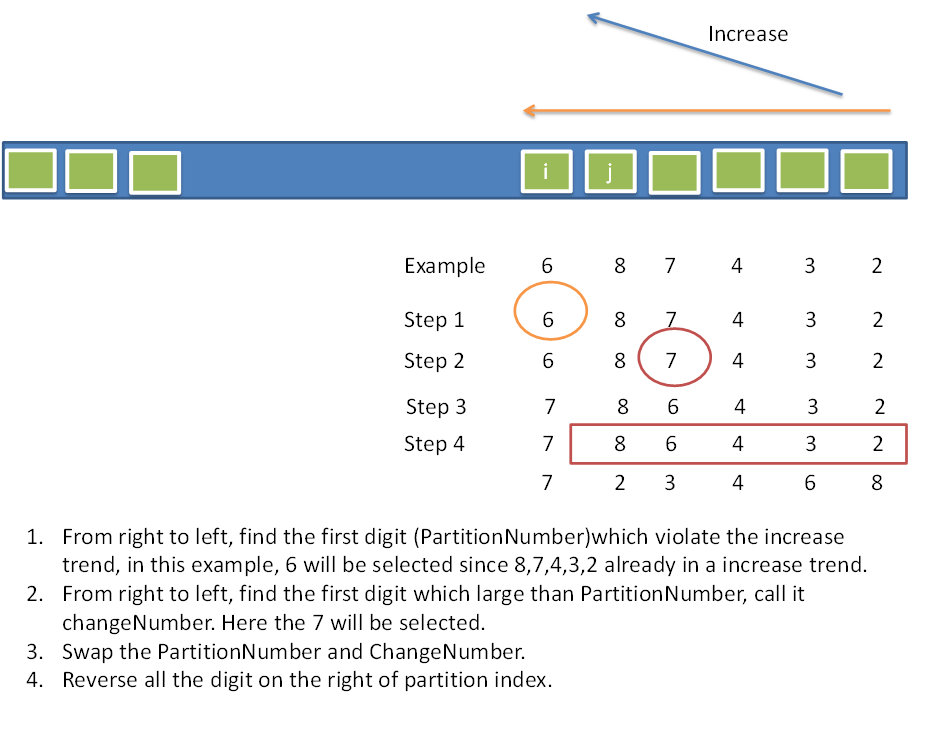
\includegraphics[width=360pt]{next-permutation.png}\\
\figcaption{下一个排列算法流程}\label{fig:permutation}
\end{center}


\subsubsection{代码}
\begin{Code}
// LeetCode, Next Permutation
// 时间复杂度O(n),空间复杂度O(1)
class Solution {
public:
    void nextPermutation(vector<int> &num) {
        next_permutation(num.begin(), num.end());
    }

    template<typename BidiIt>
    bool next_permutation(BidiIt first, BidiIt last) {
        // Get a reversed range to simplify reversed traversal.
        const auto rfirst = reverse_iterator<BidiIt>(last);
        const auto rlast = reverse_iterator<BidiIt>(first);

        // Begin from the second last element to the first element.
        auto pivot = next(rfirst);

        // Find `pivot`, which is the first element that is no less than its
        // successor.  `Prev` is used since `pivort` is a `reversed_iterator`.
        while (pivot != rlast and !(*pivot < *prev(pivot)))
            ++pivot;

        // No such elemenet found, current sequence is already the largest
        // permutation, then rearrange to the first permutation and return false.
        if (pivot == rlast) {
            reverse(rfirst, rlast);
            return false;
        }

        // Scan from right to left, find the first element that is greater than
        // `pivot`.
        auto change = find_if(rfirst, pivot, bind1st(less<int>(), *pivot));

        swap(*change, *pivot);
        reverse(rfirst, pivot);

        return true;
    }
};
\end{Code}


\subsubsection{相关题目}
\begindot
\item Permutation Sequence, 见 \S \ref{sec:permutation-sequence}
\item Permutations, 见 \S \ref{sec:permutations}
\item Permutations II, 见 \S \ref{sec:permutations-ii}
\item Combinations, 见 \S \ref{sec:combinations}
\myenddot


\subsection{Permutation Sequence} %%%%%%%%%%%%%%%%%%%%%%%%%%%%%%
\label{sec:permutation-sequence}


\subsubsection{描述}
The set \fn{[1,2,3,…,n]} contains a total of $n!$ unique permutations.

By listing and labeling all of the permutations in order,
We get the following sequence (ie, for $n = 3$):
\begin{Code}
"123"
"132"
"213"
"231"
"312"
"321"
\end{Code}

Given $n$ and $k$, return the kth permutation sequence.

Note: Given $n$ will be between 1 and 9 inclusive.


\subsubsection{分析}
简单的,可以用暴力枚举法,调用 $k-1$ 次 \fn{next_permutation()}。

暴力枚举法把前 $k$个排列都求出来了,比较浪费,而我们只需要第$k$个排列。

利用康托编码的思路,假设有$n$个不重复的元素,第$k$个排列是$a_1, a_2, a_3, ..., a_n$,那么$a_1$是哪一个位置呢?

我们把$a_1$去掉,那么剩下的排列为
$a_2, a_3, ..., a_n$, 共计$n-1$个元素,$n-1$个元素共有$(n-1)!$个排列,于是就可以知道 $a_1 = k / (n-1)!$。

同理,$a_2, a_3, ..., a_n$的值推导如下:

\begin{eqnarray}
k_2 &=& k\%(n-1)! \nonumber \\
a_2 &=& k_2/(n-2)! \nonumber \\
... &=& ... \nonumber \\
k_{n-1} &=& k_{n-2}\%2! \nonumber \\
a_{n-1} &=& k_{n-1}/1! \nonumber \\
a_n &=& 0 \nonumber
\end{eqnarray}


\subsubsection{使用next_permutation()}
\begin{Code}
// LeetCode, Permutation Sequence
// 使用next_permutation(),TLE
class Solution {
public:
    string getPermutation(int n, int k) {
        string s(n, '0');
        for (int i = 0; i < n; ++i)
            s[i] += i+1;
        for (int i = 0; i < k-1; ++i)
            next_permutation(s.begin(), s.end());
        return s;
    }

    template<typename BidiIt>
    bool next_permutation(BidiIt first, BidiIt last) {
        // 代码见上一题 Next Permutation
    }
};
\end{Code}


\subsubsection{康托编码}
\begin{Code}
// LeetCode, Permutation Sequence
// 康托编码,时间复杂度O(n),空间复杂度O(1)
class Solution {
public:
    string getPermutation(int n, int k) {
        string s(n, '0');
        string result;
        for (int i = 0; i < n; ++i)
            s[i] += i + 1;

        return kth_permutation(s, k);
    }
private:
    int factorial(int n) {
        int result = 1;
        for (int i = 1; i <= n; ++i)
            result *= i;
        return result;
    }

    // seq 已排好序,是第一个排列
    template<typename Sequence>
    Sequence kth_permutation(const Sequence &seq, int k) {
        const int n = seq.size();
        Sequence S(seq);
        Sequence result;

        int base = factorial(n - 1);
        --k;  // 康托编码从0开始

        for (int i = n - 1; i > 0; k %= base, base /= i, --i) {
            auto pos = next(S.begin(), k / base);
            result.push_back(*pos);
            S.erase(pos);
        }

        result.push_back(S[0]); // 最后一个
        return result;
    }
};
\end{Code}


\subsubsection{相关题目}
\begindot
\item Next Permutation, 见 \S \ref{sec:next-permutation}
\item Permutations, 见 \S \ref{sec:permutations}
\item Permutations II, 见 \S \ref{sec:permutations-ii}
\item Combinations, 见 \S \ref{sec:combinations}
\myenddot


\subsection{Valid Sudoku} %%%%%%%%%%%%%%%%%%%%%%%%%%%%%%
\label{sec:valid-sudoku}


\subsubsection{描述}
Determine if a Sudoku is valid, according to: Sudoku Puzzles - The Rules \myurl{http://sudoku.com.au/TheRules.aspx} .

The Sudoku board could be partially filled, where empty cells are filled with the character \fn{'.'}.

\begin{center}
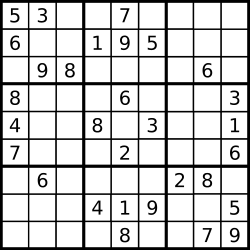
\includegraphics[width=200pt]{sudoku.png}\\
\figcaption{A partially filled sudoku which is valid}\label{fig:sudoku}
\end{center}

\subsubsection{分析}
细节实现题。


\subsubsection{代码}
\begin{Code}
// LeetCode, Valid Sudoku
// 时间复杂度O(n^2),空间复杂度O(1)
class Solution {
public:
    bool isValidSudoku(vector<vector<char>>& board) {
        bool used[9];

        for (int i = 0; i < 9; ++i) {
            fill(used, used + 9, false);

            for (int j = 0; j < 9; ++j) // 检查行
                if (!check(board[i][j], used))
                    return false;

            fill(used, used + 9, false);

            for (int j = 0; j < 9; ++j) // 检查列
                if (!check(board[j][i], used))
                    return false;
        }

        for (int r = 0; r < 3; ++r) // 检查 9 个子格子
            for (int c = 0; c < 3; ++c) {
                fill(used, used + 9, false);

                for (int i = r * 3; i < r * 3 + 3; ++i)
                    for (int j = c * 3; j < c * 3 + 3; ++j)
                        if (!check(board[i][j], used))
                            return false;
            }

        return true;
    }

    bool check(char ch, bool used[9]) {
        if (ch == '.') return true;

        if (used[ch - '1']) return false;

        used[ch - '1'] = true;
        return true;
    }
};
\end{Code}


\subsubsection{相关题目}
\begindot
\item Sudoku Solver, 见 \S \ref{sec:sudoku-solver}
\myenddot


\subsection{Trapping Rain Water} %%%%%%%%%%%%%%%%%%%%%%%%%%%%%%
\label{sec:trapping-rain-water}


\subsubsection{描述}
Given $n$ non-negative integers representing an elevation map where the width of each bar is 1, compute how much water it is able to trap after raining.

For example, 
Given \code{[0,1,0,2,1,0,1,3,2,1,2,1]}, return 6.

\begin{center}
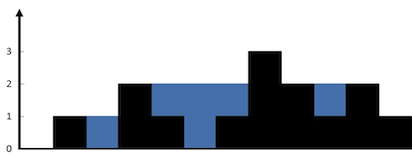
\includegraphics{trapping-rain-water.png}\\
\figcaption{Trapping Rain Water}\label{fig:trapping-rain-water}
\end{center}


\subsubsection{分析}
对于每个柱子,找到其左右两边最高的柱子,该柱子能容纳的面积就是\code{min(max_left, max_right) - height}。所以,
\begin{enumerate}
\item 从左往右扫描一遍,对于每个柱子,求取左边最大值;
\item 从右往左扫描一遍,对于每个柱子,求最大右值;
\item 再扫描一遍,把每个柱子的面积并累加。
\end{enumerate}

也可以,
\begin{enumerate}
\item 扫描一遍,找到最高的柱子,这个柱子将数组分为两半;
\item 处理左边一半;
\item 处理右边一半。
\end{enumerate}


\subsubsection{代码1}
\begin{Code}
// LeetCode, Trapping Rain Water
// 思路1,时间复杂度O(n),空间复杂度O(n)
class Solution {
public:
    int trap(int A[], int n) {
        int *max_left = new int[n]();
        int *max_right = new int[n]();

        for (int i = 1; i < n; i++) {
            max_left[i] = max(max_left[i - 1], A[i - 1]);
            max_right[n - 1 - i] = max(max_right[n - i], A[n - i]);

        }

        int sum = 0;
        for (int i = 0; i < n; i++) {
            int height = min(max_left[i], max_right[i]);
            if (height > A[i]) {
                sum += height - A[i];
            }
        }

        delete[] max_left;
        delete[] max_right;
        return sum;
    }
};
\end{Code}


\subsubsection{代码2}
\begin{Code}
// LeetCode, Trapping Rain Water
// 思路2,时间复杂度O(n),空间复杂度O(1)
class Solution {
public:
    int trap(int A[], int n) {
        int max = 0; // 最高的柱子,将数组分为两半
        for (int i = 0; i < n; i++)
            if (A[i] > A[max]) max = i;

        int water = 0;
        for (int i = 0, peak = 0; i < max; i++)
            if (A[i] > peak) peak = A[i];
            else water += peak - A[i];
        for (int i = n - 1, top = 0; i > max; i--)
            if (A[i] > top) top = A[i];
            else water += top - A[i];
        return water;
    }
};
\end{Code}


\subsubsection{代码3}
第三种解法,用一个栈辅助,小于栈顶的元素压入,大于等于栈顶就把栈里所有小于或等于当前值的元素全部出栈处理掉。
\begin{Code}
// LeetCode, Trapping Rain Water
// 用一个栈辅助,小于栈顶的元素压入,大于等于栈顶就把栈里所有小于或
// 等于当前值的元素全部出栈处理掉,计算面积,最后把当前元素入栈
// 时间复杂度O(n),空间复杂度O(n)
class Solution {
public:
    int trap(int a[], int n) {
        stack<pair<int, int>> s;
        int water = 0;

        for (int i = 0; i < n; ++i) {
            int height = 0;

            while (!s.empty()) { // 将栈里比当前元素矮或等高的元素全部处理掉
                int bar = s.top().first;
                int pos = s.top().second;
                // bar, height, a[i] 三者夹成的凹陷
                water += (min(bar, a[i]) - height) * (i - pos - 1);
                height = bar;

                if (a[i] < bar) // 碰到了比当前元素高的,跳出循环
                    break;
                else
                    s.pop(); // 弹出栈顶,因为该元素处理完了,不再需要了
            }

            s.push(make_pair(a[i], i));
        }

        return water;
    }
};
\end{Code}


\subsubsection{相关题目}
\begindot
\item Container With Most Water, 见 \S \ref{sec:container-with-most-water}
\item Largest Rectangle in Histogram, 见 \S \ref{sec:largest-rectangle-in-histogram}
\myenddot


\subsection{Rotate Image} %%%%%%%%%%%%%%%%%%%%%%%%%%%%%%
\label{sec:rotate-image}


\subsubsection{描述}
You are given an $n \times n$ 2D matrix representing an image.

Rotate the image by 90 degrees (clockwise).

Follow up:
Could you do this in-place?


\subsubsection{分析}
首先想到,纯模拟,从外到内一圈一圈的转,但这个方法太慢。

如下图,首先沿着副对角线翻转一次,然后沿着水平中线翻转一次。

\begin{center}
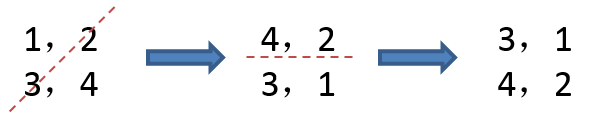
\includegraphics{rotate-image.png}\\
\figcaption{Rotate Image}\label{fig:rotate-image}
\end{center}

或者,首先沿着水平中线翻转一次,然后沿着主对角线翻转一次。


\subsubsection{代码1}
\begin{Code}
// LeetCode, Rotate Image
// 思路 1,时间复杂度O(n^2),空间复杂度O(1)
class Solution {
public:
    void rotate(vector<vector<int>>& matrix) {
        const int n = matrix.size();

        for (int i = 0; i < n; ++i)  // 沿着副对角线反转
            for (int j = 0; j < n - i; ++j)
                swap(matrix[i][j], matrix[n - 1 - j][n - 1 - i]);

        for (int i = 0; i < n / 2; ++i) // 沿着水平中线反转
            for (int j = 0; j < n; ++j)
                swap(matrix[i][j], matrix[n - 1 - i][j]);
    }
};
\end{Code}

\subsubsection{代码2}
\begin{Code}
// LeetCode, Rotate Image
// 思路 2,时间复杂度O(n^2),空间复杂度O(1)
class Solution {
public:
    void rotate(vector<vector<int>>& matrix) {
        const int n = matrix.size();

        for (int i = 0; i < n / 2; ++i) // 沿着水平中线反转
            for (int j = 0; j < n; ++j)
                swap(matrix[i][j], matrix[n - 1 - i][j]);

        for (int i = 0; i < n; ++i)  // 沿着主对角线反转
            for (int j = i + 1; j < n; ++j)
                swap(matrix[i][j], matrix[j][i]);
    }
};
\end{Code}


\subsubsection{相关题目}
\begindot
\item 无
\myenddot


\subsection{Plus One} %%%%%%%%%%%%%%%%%%%%%%%%%%%%%%
\label{sec:plus-one}


\subsubsection{描述}
Given a number represented as an array of digits, plus one to the number.


\subsubsection{分析}
高精度加法。


\subsubsection{代码1}
\begin{Code}
// LeetCode, Plus One
// 时间复杂度O(n),空间复杂度O(1)
class Solution {
public:
    vector<int> plusOne(vector<int> &digits) {
        add(digits, 1);
        return digits;
    }
private:
    // 0 <= digit <= 9
    void add(vector<int> &digits, int digit) {
        int carry = digit;

        for (auto it = digits.rbegin(); it != digits.rend(); ++it) {
            *it += carry;
            carry = *it / 10;
            *it %= 10;
        }

        if (carry > 0) digits.insert(digits.begin(), 1);
    }
};
\end{Code}


\subsubsection{代码2}
\begin{Code}
// LeetCode, Plus One
// 时间复杂度O(n),空间复杂度O(1)
class Solution {
public:
    vector<int> plusOne(vector<int> &digits) {
        add(digits, 1);
        return digits;
    }
private:
    // 0 <= digit <= 9
    void add(vector<int> &digits, int digit) {
        int carry = digit;

        for_each(digits.rbegin(), digits.rend(), [&carry](int &d){
            d += carry;
            carry = d / 10;
            d %= 10;
        });

        if (carry > 0) digits.insert(digits.begin(), 1);
    }
};
\end{Code}


\subsubsection{相关题目}
\begindot
\item 无
\myenddot


\subsection{Climbing Stairs} %%%%%%%%%%%%%%%%%%%%%%%%%%%%%%
\label{sec:climbing-stairs}


\subsubsection{描述}
You are climbing a stair case. It takes $n$ steps to reach to the top.

Each time you can either climb 1 or 2 steps. In how many distinct ways can you climb to the top?


\subsubsection{分析}
设$f(n)$表示爬$n$阶楼梯的不同方法数,为了爬到第$n$阶楼梯,有两个选择:
\begindot
\item 从第$n-1$阶前进1步;
\item 从第$n-1$阶前进2步;
\myenddot
因此,有$f(n)=f(n-1)+f(n-2)$。

这是一个斐波那契数列。


\subsubsection{迭代}
\begin{Code}
// LeetCode, Climbing Stairs
// 迭代,时间复杂度O(n),空间复杂度O(1)
class Solution {
public:
    int climbStairs(int n) {
        int prev = 0;
        int cur = 1;
        for(int i = 1; i <= n ; ++i){
            int tmp = cur;
            cur = prev + cur;
            prev = tmp;
        }
        return cur;
    }
};
\end{Code}


\subsubsection{数学公式}
\begin{Code}
// LeetCode, Climbing Stairs
// 数学公式,时间复杂度O(1),空间复杂度O(1)
class Solution {
    public:
    int climbStairs(int n) {
        double s = sqrt(5);
        return floor((pow((1+s)/2, n+1) + pow((1-s)/2, n+1))/s + 0.5);
    }
};
\end{Code}


\subsubsection{相关题目}
\begindot
\item Decode Ways, 见 \S \ref{sec:decode-ways}
\myenddot


\subsection{Gray Code} %%%%%%%%%%%%%%%%%%%%%%%%%%%%%%
\label{sec:gray-code}


\subsubsection{描述}
The gray code is a binary numeral system where two successive values differ in only one bit.

Given a non-negative integer $n$ representing the total number of bits in the code, print the sequence of gray code. A gray code sequence must begin with 0.

For example, given $n = 2$, return \fn{[0,1,3,2]}. Its gray code sequence is:
\begin{Code}
00 - 0
01 - 1
11 - 3
10 - 2
\end{Code}

Note:
\begindot
\item For a given $n$, a gray code sequence is not uniquely defined.
\item For example, \fn{[0,2,3,1]} is also a valid gray code sequence according to the above definition.
\item For now, the judge is able to judge based on one instance of gray code sequence. Sorry about that.
\myenddot


\subsubsection{分析}
格雷码(Gray Code)的定义请参考 wikipedia \myurl{http://en.wikipedia.org/wiki/Gray_code}。

\textbf{自然二进制码转换为格雷码:$g_0=b_0, g_i=b_i \oplus b_{i-1}$}

保留自然二进制码的最高位作为格雷码的最高位,格雷码次高位为二进制码的高位与次高位异或,其余各位与次高位的求法类似。例如,将自然二进制码1001,转换为格雷码的过程是:保留最高位;然后将第1位的1和第2位的0异或,得到1,作为格雷码的第2位;将第2位的0和第3位的0异或,得到0,作为格雷码的第3位;将第3位的0和第4位的1异或,得到1,作为格雷码的第4位,最终,格雷码为1101。

\textbf{格雷码转换为自然二进制码:$b_0=g_0, b_i=g_i \oplus b_{i-1}$}

保留格雷码的最高位作为自然二进制码的最高位,次高位为自然二进制高位与格雷码次高位异或,其余各位与次高位的求法类似。例如,将格雷码1000转换为自然二进制码的过程是:保留最高位1,作为自然二进制码的最高位;然后将自然二进制码的第1位1和格雷码的第2位0异或,得到1,作为自然二进制码的第2位;将自然二进制码的第2位1和格雷码的第3位0异或,得到1,作为自然二进制码的第3位;将自然二进制码的第3位1和格雷码的第4位0异或,得到1,作为自然二进制码的第4位,最终,自然二进制码为1111。

格雷码有\textbf{数学公式},整数$n$的格雷码是$n \oplus (n/2)$。

这题要求生成$n$比特的所有格雷码。

最简单的方法,利用数学公式,对从 $0\sim2^n-1$的所有整数,转化为格雷码。

$n$比特的格雷码,可以递归地从$n-1$比特的格雷码生成。如图\S \ref{fig:gray-code-construction}所示。

\begin{center}
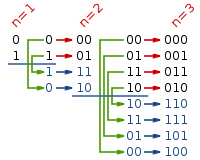
\includegraphics{gray-code-construction.png}\\
\figcaption{The first few steps of the reflect-and-prefix method.}\label{fig:gray-code-construction}
\end{center}


\subsubsection{数学公式}
\begin{Code}
// LeetCode, Gray Code
// 数学公式,时间复杂度O(2^n),空间复杂度O(1)
class Solution {
public:
    vector<int> grayCode(int n) {
        vector<int> result;
        const size_t size = 1 << n;  // 2^n
        result.reserve(size);
        for (size_t i = 0; i < size; ++i)
            result.push_back(binary_to_gray(i));
        return result;
    }
private:
    static unsigned int binary_to_gray(unsigned int n) {
        return n ^ (n >> 1);
    }
    static unsigned int gray_to_binary(unsigned int g) {
        for (unsigned int mask = g >> 1; mask != 0; mask = mask >> 1)
            g = g ^ mask;
        return g;
    }
};
\end{Code}


\subsubsection{Reflect-and-prefix method}
\begin{Code}
// LeetCode, Gray Code
// reflect-and-prefix method
// 时间复杂度O(2^n),空间复杂度O(1)
class Solution {
public:
    vector<int> grayCode(int n) {
        vector<int> result;
        result.push_back(0);
        for (int i = 0; i < n; i++) {
            const int highest_bit = 1 << i;
            for (int j = result.size() - 1; j >= 0; j--) // 要反着遍历,才能对称
                result.push_back(highest_bit | result[j]);
        }
        return result;
    }
};
\end{Code}


\subsubsection{相关题目}
\begindot
\item 无
\myenddot


\subsection{Set Matrix Zeroes} %%%%%%%%%%%%%%%%%%%%%%%%%%%%%%
\label{sec:set-matrix-zeroes}


\subsubsection{描述}
Given a $m \times n$ matrix, if an element is 0, set its entire row and column to 0. Do it in place.

\textbf{Follow up:}
Did you use extra space?

A straight forward solution using $O(mn)$ space is probably a bad idea.

A simple improvement uses $O(m + n)$ space, but still not the best solution.

Could you devise a constant space solution?


\subsubsection{分析}
$O(m+n)$空间的方法很简单,设置两个数组,记录每行和每列是否存在0。

想要常数空间,可以复用第一行和第一列。


\subsubsection{代码1}
\begin{Code}
// LeetCode, Set Matrix Zeroes
// 时间复杂度O(m*n),空间复杂度O(m+n)
class Solution {
public:
    void setZeroes(vector<vector<int> > &matrix) {
        const size_t m = matrix.size();
        const size_t n = matrix[0].size();
        vector<bool> row(m, false); // 标记该行是否存在0
        vector<bool> col(n, false); // 标记该列是否存在0

        for (size_t i = 0; i < m; ++i) {
            for (size_t j = 0; j < n; ++j) {
                if (matrix[i][j] == 0) {
                    row[i] = col[j] = true;
                }
            }
        }

        for (size_t i = 0; i < m; ++i) {
            if (row[i])
                fill(&matrix[i][0], &matrix[i][0] + n, 0);
        }
        for (size_t j = 0; j < n; ++j) {
            if (col[j]) {
                for (size_t i = 0; i < m; ++i) {
                    matrix[i][j] = 0;
                }
            }
        }
    }
};
\end{Code}


\subsubsection{代码2}
\begin{Code}
// LeetCode, Set Matrix Zeroes
// 时间复杂度O(m*n),空间复杂度O(1)
class Solution {
public:
    void setZeroes(vector<vector<int> > &matrix) {
        const size_t m = matrix.size();
        const size_t n = matrix[0].size();
        bool row_has_zero = false; // 第一行是否存在 0
        bool col_has_zero = false; // 第一列是否存在 0

        for (size_t i = 0; i < n; i++)
            if (matrix[0][i] == 0) {
                row_has_zero = true;
                break;
            }

        for (size_t i = 0; i < m; i++)
            if (matrix[i][0] == 0) {
                col_has_zero = true;
                break;
            }

        for (size_t i = 1; i < m; i++)
            for (size_t j = 1; j < n; j++)
                if (matrix[i][j] == 0) {
                    matrix[0][j] = 0;
                    matrix[i][0] = 0;
                }
        for (size_t i = 1; i < m; i++)
            for (size_t j = 1; j < n; j++)
                if (matrix[i][0] == 0 || matrix[0][j] == 0)
                    matrix[i][j] = 0;
        if (row_has_zero)
            for (size_t i = 0; i < n; i++)
                matrix[0][i] = 0;
        if (col_has_zero)
            for (size_t i = 0; i < m; i++)
                matrix[i][0] = 0;
    }
};
\end{Code}


\subsubsection{相关题目}
\begindot
\item 无
\myenddot


\subsection{Gas Station} %%%%%%%%%%%%%%%%%%%%%%%%%%%%%%
\label{sec:gas-station}


\subsubsection{描述}
There are $N$ gas stations along a circular route, where the amount of gas at station $i$ is \fn{gas[i]}.

You have a car with an unlimited gas tank and it costs \fn{cost[i]} of gas to travel from station $i$ to its next station ($i$+1). You begin the journey with an empty tank at one of the gas stations.

Return the starting gas station's index if you can travel around the circuit once, otherwise return -1.

Note:
The solution is guaranteed to be unique.


\subsubsection{分析}
首先想到的是$O(N^2)$的解法,对每个点进行模拟。

$O(N)$的解法是,设置两个变量,\fn{sum}判断当前的指针的有效性;\fn{total}则判断整个数组是否有解,有就返回通过\fn{sum}得到的下标,没有则返回-1。


\subsubsection{代码}
\begin{Code}
// LeetCode, Gas Station
// 时间复杂度O(n),空间复杂度O(1)
class Solution {
public:
    int canCompleteCircuit(vector<int> &gas, vector<int> &cost) {
        int total = 0;
        int j = -1;
        for (int i = 0, sum = 0; i < gas.size(); ++i) {
            sum += gas[i] - cost[i];
            total += gas[i] - cost[i];
            if (sum < 0) {
                j = i;
                sum = 0;
            }
        }
        return total >= 0 ? j + 1 : -1;
    }
};
\end{Code}


\subsubsection{相关题目}
\begindot
\item 无
\myenddot


\subsection{Candy} %%%%%%%%%%%%%%%%%%%%%%%%%%%%%%
\label{sec:candy}


\subsubsection{描述}
There are $N$ children standing in a line. Each child is assigned a rating value.

You are giving candies to these children subjected to the following requirements:
\begindot
\item Each child must have at least one candy.
\item Children with a higher rating get more candies than their neighbors.
\myenddot

What is the minimum candies you must give?


\subsubsection{分析}
无


\subsubsection{代码}
\begin{Code}
// LeetCode, Candy
// 时间复杂度O(n),空间复杂度O(n)
class Solution {
public:
    int candy(vector<int> &ratings) {
        const int n = ratings.size();
        int result = n;
        vector<int> increment(n);

        // 左右各扫描一遍
        for (int i = 0, inc = 1; i < n; i++)
            if (i >= 1 && ratings[i] > ratings[i - 1])
                increment[i] = max(inc++, increment[i]);
            else
                inc = 1;

        for (int i = n - 1, inc = 1; i >= 0; i--)
            if (i < n - 1 && ratings[i] > ratings[i + 1])
                increment[i] = max(inc++, increment[i]);
            else
                inc = 1;

        for (int i = 0; i < n; i++)
            result += increment[i];

        return result;
    }
};
\end{Code}


\subsubsection{相关题目}
\begindot
\item 无
\myenddot


\subsection{Single Number} %%%%%%%%%%%%%%%%%%%%%%%%%%%%%%
\label{sec:single-number}


\subsubsection{描述}
Given an array of integers, every element appears twice except for one. Find that single one.

Note:
Your algorithm should have a linear runtime complexity. Could you implement it without using extra memory?


\subsubsection{分析}
异或,不仅能处理两次的情况,只要出现偶数次,都可以清零。


\subsubsection{代码}
\begin{Code}
// LeetCode, Single Number
// 时间复杂度O(n),空间复杂度O(1)
class Solution {
public:
    int singleNumber(int A[], int n) {
        int x = A[0];
        for (size_t i = 1; i < n; ++i)
            x ^= A[i];
        return x;
    }
};
\end{Code}


\subsubsection{相关题目}
\begindot
\item  Single Number II, 见 \S \ref{sec:single-number-ii}
\myenddot


\subsection{Single Number II} %%%%%%%%%%%%%%%%%%%%%%%%%%%%%%
\label{sec:single-number-ii}


\subsubsection{描述}
Given an array of integers, every element appears three times except for one. Find that single one.

Note:
Your algorithm should have a linear runtime complexity. Could you implement it without using extra memory?


\subsubsection{分析}
本题和上一题 Single Number,考察的是位运算。

方法1:创建一个长度为\fn{sizeof(int)}的数组\fn{count[sizeof(int)]},\fn{count[i]}表示所有元素的1在$i$位出现的次数。如果\fn{count[i]}是3的整数倍,则忽略;否则就把该位取出来组成答案。

方法2:用\fn{ones}记录到当前处理的元素为止,二进制1出现“1次”(mod 3 之后的 1)的有哪些二进制位;用\fn{twos}记录到当前计算的变量为止,二进制1出现“2次”(mod 3 之后的 2)的有哪些二进制位。当\fn{ones}和\fn{twos}中的某一位同时为1时表示该二进制位上1出现了3次,此时需要清零。即\textbf{用二进制模拟三进制运算}。最终\fn{ones}记录的是最终结果。

\subsubsection{代码1}
\begin{Code}
// LeetCode, Single Number II
// 方法1,时间复杂度O(n),空间复杂度O(1)
class Solution {
public:
    int singleNumber(int A[], int n) {
        const int W = sizeof(int) * 8; // 整数字长
        int count[W];  // 每个位上1出现的次数
        fill_n(&count[0], W, 0);
        for (int i = 0; i < n; i++) {
            for (int j = 0; j < W; j++) {
                count[j] += (A[i] >> j) & 1;
                count[j] %= 3;
            }
        }
        int result = 0;
        for (int i = 0; i < W; i++) {
            result += (count[i] << i);
        }
        return result;
    }
};
\end{Code}


\subsubsection{代码2}
\begin{Code}
// LeetCode, Single Number II
// 方法2,时间复杂度O(n),空间复杂度O(1)
class Solution {
public:
    int singleNumber(int A[], int n) {
        int ones = 0, twos = 0, threes = 0;
        for (int i = 0; i < n; ++i) {
            twos |= (ones & A[i]);
            ones ^= A[i];
            threes = ~(ones & twos);
            ones &= threes;
            twos &= threes;
        }

        return ones;
    }
};
\end{Code}


\subsubsection{相关题目}
\begindot
\item  Single Number, 见 \S \ref{sec:single-number}
\myenddot


\section{单链表} %%%%%%%%%%%%%%%%%%%%%%%%%%%%%%

单链表节点的定义如下:
\begin{Code}
// 单链表节点
struct ListNode {
    int val;
    ListNode *next;
    ListNode(int x) : val(x), next(nullptr) { }
};
\end{Code}


\subsection{Add Two Numbers}
\label{sec:add-two-numbers}


\subsubsection{描述}
You are given two linked lists representing two non-negative numbers. The digits are stored in reverse order and each of their nodes contain a single digit. Add the two numbers and return it as a linked list.

Input: {\small \fontspec{Latin Modern Mono} (2 -> 4 -> 3) + (5 -> 6 -> 4)}

Output: {\small \fontspec{Latin Modern Mono} 7 -> 0 -> 8}


\subsubsection{分析}
跟Add Binary(见 \S \ref{sec:add-binary})很类似


\subsubsection{代码}
\begin{Code}
// LeetCode, Add Two Numbers
// 跟Add Binary 很类似
// 时间复杂度O(m+n),空间复杂度O(1)
class Solution {
public:
    ListNode *addTwoNumbers(ListNode *l1, ListNode *l2) {
        ListNode head(-1); // 头节点
        int carry = 0;
        ListNode *prev = &head;
        for (ListNode *pa = l1, *pb = l2;
             pa != nullptr || pb != nullptr;
             pa = pa == nullptr ? nullptr : pa->next,
             pb = pb == nullptr ? nullptr : pb->next,
             prev = prev->next) {
            const int ai = pa == nullptr ? 0 : pa->val;
            const int bi = pb == nullptr ? 0 : pb->val;
            const int value = (ai + bi + carry) % 10;
            carry = (ai + bi + carry) / 10;
            prev->next = new ListNode(value); // 尾插法
        }
        if (carry > 0)
            prev->next = new ListNode(carry);
        return head.next;
    }
};
\end{Code}


\subsubsection{相关题目}

\begindot
\item Add Binary, 见 \S \ref{sec:add-binary}
\myenddot


\subsection{Reverse Linked List II}
\label{sec:reverse-linked-list-ii}


\subsubsection{描述}
Reverse a linked list from position $m$ to $n$. Do it in-place and in one-pass.

For example:
Given \code{1->2->3->4->5->nullptr}, $m$ = 2 and $n$ = 4,

return \code{1->4->3->2->5->nullptr}.

Note:
Given m, n satisfy the following condition:
$1 \leq m \leq  n \leq $ length of list.


\subsubsection{分析}
这题非常繁琐,有很多边界检查,15分钟内做到bug free很有难度!


\subsubsection{代码}
\begin{Code}
// LeetCode, Reverse Linked List II
// 迭代版,时间复杂度O(n),空间复杂度O(1)
class Solution {
public:
    ListNode *reverseBetween(ListNode *head, int m, int n) {
        ListNode dummy(-1);
        dummy.next = head;

        ListNode *prev_m, *prev = &dummy;
        for (int i = 1; i <= n; ++i) {
            if (i == m) prev_m = prev;

            if (i > m && i <= n) { // prev_m 和 prev 静止不动
                prev->next = head->next;
                head->next = prev_m->next;
                prev_m->next = head;
                head = prev;
            }

            prev = head;
            head = head->next;
        }

        return dummy.next;
    }
};
\end{Code}


\subsubsection{相关题目}

\begindot
\item 无
\myenddot


\subsection{Partition List}
\label{sec:partition-list}


\subsubsection{描述}
Given a linked list and a value $x$, partition it such that all nodes less than $x$ come before nodes greater than or equal to $x$.

You should preserve the original relative order of the nodes in each of the two partitions.

For example,
Given \code{1->4->3->2->5->2} and \code{x = 3}, return \code{1->2->2->4->3->5}.


\subsubsection{分析}
无


\subsubsection{代码}
\begin{Code}
// LeetCode, Partition List
// 时间复杂度O(n),空间复杂度O(1)
class Solution {
public:
    ListNode* partition(ListNode* head, int x) {
        if (head == nullptr) return head;

        ListNode left_dummy(0); // 头结点
        ListNode right_dummy(0); // 头结点

        auto left_cur = &left_dummy;
        auto right_cur = &right_dummy;

        for (; head; head = head->next) {
            if (head->val < x) {
                left_cur->next = head;
                left_cur = head;
            } else {
                right_cur->next = head;
                right_cur = head;
            }
        }

        left_cur->next = right_dummy.next;
        right_cur->next = nullptr;

        return left_dummy.next;
    }
};
\end{Code}


\subsubsection{相关题目}

\begindot
\item 无
\myenddot


\subsection{Remove Duplicates from Sorted List}
\label{sec:remove-duplicates-from-sorted-list}


\subsubsection{描述}
Given a sorted linked list, delete all duplicates such that each element appear only once.

For example,

Given \code{1->1->2}, return \code{1->2}.

Given \code{1->1->2->3->3}, return \code{1->2->3}.


\subsubsection{分析}
无


\subsubsection{递归版}
\begin{Code}
// LeetCode, Remove Duplicates from Sorted List
// 递归版,时间复杂度O(n),空间复杂度O(1)
class Solution {
public:
    ListNode *deleteDuplicates(ListNode *head) {
        if (!head) return head;
        ListNode dummy(head->val + 1); // 值只要跟head不同即可
        dummy.next = head;

        recur(&dummy, head);
        return dummy.next;
    }
private:
    static void recur(ListNode *prev, ListNode *cur) {
        if (cur == nullptr) return;

        if (prev->val == cur->val) { // 删除head
            prev->next = cur->next;
            delete cur;
            recur(prev, prev->next);
        } else {
            recur(prev->next, cur->next);
        }
    }
};
\end{Code}


\subsubsection{迭代版}
\begin{Code}
// LeetCode, Remove Duplicates from Sorted List
// 迭代版,时间复杂度O(n),空间复杂度O(1)
class Solution {
public:
    ListNode *deleteDuplicates(ListNode *head) {
        if (head == nullptr) return nullptr;

        for (ListNode *prev = head, *cur = head->next; cur; cur = cur->next) {
            if (prev->val == cur->val) {
                prev->next = cur->next;
                delete cur;
            } else {
                prev = cur;
            }
        }
        return head;
    }
};
\end{Code}


\subsubsection{相关题目}

\begindot
\item Remove Duplicates from Sorted List II,见 \S \ref{sec:remove-duplicates-from-sorted-list-ii}
\myenddot


\subsection{Remove Duplicates from Sorted List II}
\label{sec:remove-duplicates-from-sorted-list-ii}


\subsubsection{描述}
Given a sorted linked list, delete all nodes that have duplicate numbers, leaving only distinct numbers from the original list.

For example,

Given \code{1->2->3->3->4->4->5}, return \code{1->2->5}.

Given \code{1->1->1->2->3}, return \code{2->3}.


\subsubsection{分析}
无


\subsubsection{递归版}
\begin{Code}
// LeetCode, Remove Duplicates from Sorted List II
// 递归版,时间复杂度O(n),空间复杂度O(1)
class Solution {
public:
    ListNode *deleteDuplicates(ListNode *head) {
        if (!head || !head->next) return head;

        ListNode *p = head->next;
        if (head->val == p->val) {
            while (p && head->val == p->val) {
                ListNode *tmp = p;
                p = p->next;
                delete tmp;
            }
            delete head;
            return deleteDuplicates(p);
        } else {
            head->next = deleteDuplicates(head->next);
            return head;
        }
    }
};
\end{Code}


\subsubsection{迭代版}
\begin{Code}
// LeetCode, Remove Duplicates from Sorted List II
// 迭代版,时间复杂度O(n),空间复杂度O(1)
class Solution {
public:
    ListNode *deleteDuplicates(ListNode *head) {
        if (head == nullptr) return head;

        ListNode dummy(INT_MIN); // 头结点
        dummy.next = head;
        ListNode *prev = &dummy, *cur = head;
        while (cur != nullptr) {
            bool duplicated = false;
            while (cur->next != nullptr && cur->val == cur->next->val) {
                duplicated = true;
                ListNode *temp = cur;
                cur = cur->next;
                delete temp;
            }
            if (duplicated) { // 删除重复的最后一个元素
                ListNode *temp = cur;
                cur = cur->next;
                delete temp;
                continue;
            }
            prev->next = cur;
            prev = prev->next;
            cur = cur->next;
        }
        prev->next = cur;
        return dummy.next;
    }
};
\end{Code}


\subsubsection{相关题目}

\begindot
\item Remove Duplicates from Sorted List,见 \S \ref{sec:remove-duplicates-from-sorted-list}
\myenddot


\subsection{Rotate List}
\label{sec:rotate-list}


\subsubsection{描述}
Given a list, rotate the list to the right by $k$ places, where $k$ is non-negative.

For example:
Given \code{1->2->3->4->5->nullptr} and \code{k = 2}, return \code{4->5->1->2->3->nullptr}.


\subsubsection{分析}
先遍历一遍,得出链表长度$len$,注意$k$可能大于$len$,因此令$k \%= len$。将尾节点next指针指向首节点,形成一个环,接着往后跑$len-k$步,从这里断开,就是要求的结果了。


\subsubsection{代码}
\begin{Code}
// LeetCode, Remove Rotate List
// 时间复杂度O(n),空间复杂度O(1)
class Solution {
public:
    ListNode *rotateRight(ListNode *head, int k) {
        if (head == nullptr || k == 0) return head;

        int len = 1;
        ListNode* p = head;
        while (p->next) { // 求长度
            len++;
            p = p->next;
        }
        k = len - k % len;

        p->next = head; // 首尾相连
        for(int step = 0; step < k; step++) {
            p = p->next;  //接着往后跑
        }
        head = p->next; // 新的首节点
        p->next = nullptr; // 断开环
        return head;
    }
};
\end{Code}


\subsubsection{相关题目}

\begindot
\item 无
\myenddot


\subsection{Remove Nth Node From End of List}
\label{sec:remove-nth-node-from-end-of-list}


\subsubsection{描述}
Given a linked list, remove the $n^{th}$ node from the end of list and return its head.

For example, Given linked list: \code{1->2->3->4->5}, and $n$ = 2.

After removing the second node from the end, the linked list becomes \code{1->2->3->5}.

Note:
\begindot
\item Given $n$ will always be valid.
\item Try to do this in one pass.
\myenddot


\subsubsection{分析}
设两个指针$p,q$,让$q$先走$n$步,然后$p$和$q$一起走,直到$q$走到尾节点,删除\fn{p->next}即可。


\subsubsection{代码}
\begin{Code}
// LeetCode, Remove Nth Node From End of List
// 时间复杂度O(n),空间复杂度O(1)
class Solution {
public:
    ListNode *removeNthFromEnd(ListNode *head, int n) {
        ListNode dummy(0);
        dummy.next = head;
        ListNode *p = &dummy, *q = &dummy;

        for (int i = 0; i < n; i++)  // q先走n步
            q = q->next;

        while(q->next) { // 一起走
            p = p->next;
            q = q->next;
        }
        ListNode *tmp = p->next;
        p->next = p->next->next;
        delete tmp;
        return dummy.next;
    }
};
\end{Code}


\subsubsection{相关题目}

\begindot
\item 无
\myenddot


\subsection{Swap Nodes in Pairs}
\label{sec:swap-nodes-in-pairs}


\subsubsection{描述}
Given a linked list, swap every two adjacent nodes and return its head.

For example,
Given \code{1->2->3->4}, you should return the list as \code{2->1->4->3}.

Your algorithm should use only constant space. You may \emph{not} modify the values in the list, only nodes itself can be changed.


\subsubsection{分析}
无


\subsubsection{代码}
\begin{Code}
// LeetCode, Swap Nodes in Pairs
// 时间复杂度O(n),空间复杂度O(1)
class Solution {
public:
    ListNode *swapPairs(ListNode *head) {
        if (head == nullptr || head->next == nullptr) return head;
        ListNode dummy(-1);
        dummy.next = head;

        for(ListNode *prev = &dummy, *cur = prev->next, *next = cur->next;
                next;
                prev = cur, cur = cur->next, next = cur ? cur->next: nullptr) {
            prev->next = next;
            cur->next = next->next;
            next->next = cur;
        }
        return dummy.next;
    }
};
\end{Code}

下面这种写法更简洁,但题目规定了不准这样做。
\begin{Code}
// LeetCode, Swap Nodes in Pairs
// 时间复杂度O(n),空间复杂度O(1)
class Solution {
public:
    ListNode* swapPairs(ListNode* head) {
        ListNode* p = head;

        while (p && p->next) {
            swap(p->val, p->next->val);
            p = p->next->next;
        }

        return head;
    }
};
\end{Code}

\subsubsection{相关题目}

\begindot
\item Reverse Nodes in k-Group, 见 \S \ref{sec:reverse-nodes-in-k-group}
\myenddot


\subsection{Reverse Nodes in k-Group}
\label{sec:reverse-nodes-in-k-group}


\subsubsection{描述}
Given a linked list, reverse the nodes of a linked list k at a time and return its modified list.

If the number of nodes is not a multiple of $k$ then left-out nodes in the end should remain as it is.

You may not alter the values in the nodes, only nodes itself may be changed.

Only constant memory is allowed.

For example,
Given this linked list: \code{1->2->3->4->5}

For $k = 2$, you should return: \code{2->1->4->3->5}

For $k = 3$, you should return: \code{3->2->1->4->5}


\subsubsection{分析}
无


\subsubsection{递归版}
\begin{Code}
// LeetCode, Reverse Nodes in k-Group
// 递归版,时间复杂度O(n),空间复杂度O(1)
class Solution {
public:
    ListNode *reverseKGroup(ListNode *head, int k) {
        if (head == nullptr || head->next == nullptr || k < 2)
            return head;

        ListNode *next_group = head;
        for (int i = 0; i < k; ++i) {
            if (next_group)
                next_group = next_group->next;
            else
                return head;
        }
        // next_group is the head of next group
        // new_next_group is the new head of next group after reversion
        ListNode *new_next_group = reverseKGroup(next_group, k);
        ListNode *prev = NULL, *cur = head;
        while (cur != next_group) {
            ListNode *next = cur->next;
            cur->next = prev ? prev : new_next_group;
            prev = cur;
            cur = next;
        }
        return prev; // prev will be the new head of this group
    }
};
\end{Code}


\subsubsection{迭代版}
\begin{Code}
// LeetCode, Reverse Nodes in k-Group
// 迭代版,时间复杂度O(n),空间复杂度O(1)
class Solution {
public:
    ListNode *reverseKGroup(ListNode *head, int k) {
        if (head == nullptr || head->next == nullptr || k < 2) return head;
        ListNode dummy(-1);
        dummy.next = head;

        for(ListNode *prev = &dummy, *end = head; end; end = prev->next) {
            for (int i = 1; i < k && end; i++)
                end = end->next;
            if (end  == nullptr) break;  // 不足 k 个

            prev = reverse(prev, prev->next, end);
        }

        return dummy.next;
    }

    // prev 是 first 前一个元素, [begin, end] 闭区间,保证三者都不为 null
    // 返回反转后的倒数第1个元素
    ListNode* reverse(ListNode *prev, ListNode *begin, ListNode *end) {
        ListNode *end_next = end->next;
        for (ListNode *p = begin, *cur = p->next, *next = cur->next;
                cur != end_next;
                p = cur, cur = next, next = next ? next->next : nullptr) {
            cur->next = p;
        }
        begin->next = end_next;
        prev->next = end;
        return begin;
    }
};
\end{Code}


\subsubsection{相关题目}
\begindot
\item Swap Nodes in Pairs, 见 \S \ref{sec:swap-nodes-in-pairs}
\myenddot


\subsection{Copy List with Random Pointer}
\label{sec:copy-list-with-random-pointer}


\subsubsection{描述}
A linked list is given such that each node contains an additional random pointer which could point to any node in the list or null.

Return a deep copy of the list.


\subsubsection{分析}
无


\subsubsection{代码}
\begin{Code}
// LeetCode, Copy List with Random Pointer
// 两遍扫描,时间复杂度O(n),空间复杂度O(1)
class Solution {
public:
    RandomListNode *copyRandomList(RandomListNode *head) {
        if (head == nullptr) return nullptr;

        for (RandomListNode* cur = head; cur != nullptr; ) {
            RandomListNode* node = new RandomListNode(cur->label);
            node->next = cur->next;
            cur->next = node;
            cur = node->next;
        }

        for (RandomListNode* cur = head; cur != nullptr; ) {
            if (cur->random != NULL)
                cur->next->random = cur->random->next;
            cur = cur->next->next;
        }

        // 分拆两个单链表
        RandomListNode new_head(-1);
        for (RandomListNode* cur = head, *new_cur = &new_head;
                cur != nullptr; ) {
            new_cur->next = cur->next;
            new_cur = new_cur->next;
            cur->next = cur->next->next;
            cur = cur->next;
        }
        return new_head.next;
    }
};
\end{Code}


\subsubsection{相关题目}
\begindot
\item 无
\myenddot

\chapter{字符串}


\section{Valid Palindrome} %%%%%%%%%%%%%%%%%%%%%%%%%%%%%%
\label{sec:valid-palindrome}


\subsubsection{描述}
Given a string, determine if it is a palindrome, considering only alphanumeric characters and ignoring cases.

For example,\\
\code{"A man, a plan, a canal: Panama"} is a palindrome.\\
\code{"race a car"} is not a palindrome.

Note:
Have you consider that the string might be empty? This is a good question to ask during an interview.

For the purpose of this problem, we define empty string as valid palindrome.


\subsubsection{分析}
无


\subsubsection{代码}
\begin{Code}
// Leet Code, Valid Palindrome
// 时间复杂度O(n),空间复杂度O(1)
class Solution {
public:
    bool isPalindrome(string s) {
        transform(s.begin(), s.end(), s.begin(), ::tolower);
        auto left = s.begin(), right = prev(s.end());
        while (left < right) {
            if (!::isalnum(*left))  ++left;
            else if (!::isalnum(*right)) --right;
            else if (*left != *right) return false;
            else{ left++, right--; }
        }
        return true;
    }
};
\end{Code}


\subsubsection{相关题目}
\begindot
\item Palindrome Number, 见 \S \ref{sec:palindrome-number}
\myenddot


\section{Implement strStr()} %%%%%%%%%%%%%%%%%%%%%%%%%%%%%%
\label{sec:strstr}


\subsubsection{描述}
Implement strStr().

Returns a pointer to the first occurrence of needle in haystack, or null if needle is not part of haystack.


\subsubsection{分析}
暴力算法的复杂度是 $O(m*n)$,代码如下。更高效的的算法有KMP算法、Boyer-Mooer算法和Rabin-Karp算法。面试中暴力算法足够了,一定要写得没有BUG。


\subsubsection{暴力匹配}
\begin{Code}
// LeetCode, Implement strStr()
// 暴力解法,时间复杂度O(N*M),空间复杂度O(1)
class Solution {
public:
    char *strStr(const char *haystack, const char *needle) {
        // if needle is empty return the full string
        if (!*needle) return (char*) haystack;

        const char *p1;
        const char *p2;
        const char *p1_advance = haystack;
        for (p2 = &needle[1]; *p2; ++p2) {
            p1_advance++;   // advance p1_advance M-1 times
        }

        for (p1 = haystack; *p1_advance; p1_advance++) {
            char *p1_old = (char*) p1;
            p2 = needle;
            while (*p1 && *p2 && *p1 == *p2) {
                p1++;
                p2++;
            }
            if (!*p2) return p1_old;

            p1 = p1_old + 1;
        }
        return nullptr;
    }
};
\end{Code}


\subsubsection{KMP}
\begin{Code}
// LeetCode, Implement strStr()
// KMP,时间复杂度O(N+M),空间复杂度O(M)
class Solution {
public:
    char *strStr(const char *haystack, const char *needle) {
        int pos = kmp(haystack, needle);
        if (pos == -1) return nullptr;
        else return (char*)haystack + pos;
    }
private:
    /*
     * @brief 计算部分匹配表,即next数组.
     *
     * @param[in] pattern 模式串
     * @param[out] next next数组
     * @return 无
     */
    static void compute_prefix(const char *pattern, int next[]) {
        int i;
        int j = -1;
        const int m = strlen(pattern);

        next[0] = j;
        for (i = 1; i < m; i++) {
            while (j > -1 && pattern[j + 1] != pattern[i]) j = next[j];

            if (pattern[i] == pattern[j + 1]) j++;
            next[i] = j;
        }
    }

    /*
     * @brief KMP算法.
     *
     * @param[in] text 文本
     * @param[in] pattern 模式串
     * @return 成功则返回第一次匹配的位置,失败则返回-1
     */
    static int kmp(const char *text, const char *pattern) {
        int i;
        int j = -1;
        const int n = strlen(text);
        const int m = strlen(pattern);
        if (n == 0 && m == 0) return 0; /* "","" */
        if (m == 0) return 0;  /* "a","" */
        int *next = (int*)malloc(sizeof(int) * m);

        compute_prefix(pattern, next);

        for (i = 0; i < n; i++) {
            while (j > -1 && pattern[j + 1] != text[i]) j = next[j];

            if (text[i] == pattern[j + 1]) j++;
            if (j == m - 1) {
                free(next);
                return i-j;
            }
        }

        free(next);
        return -1;
    }
};
\end{Code}


\subsubsection{相关题目}
\begindot
\item String to Integer (atoi) ,见 \S \ref{sec:string-to-integer}
\myenddot


\section{String to Integer (atoi)} %%%%%%%%%%%%%%%%%%%%%%%%%%%%%%
\label{sec:string-to-integer}


\subsubsection{描述}
Implement \fn{atoi} to convert a string to an integer.

\textbf{Hint}: Carefully consider all possible input cases. If you want a challenge, please do not see below and ask yourself what are the possible input cases.

\textbf{Notes}: It is intended for this problem to be specified vaguely (ie, no given input specs). You are responsible to gather all the input requirements up front.

\textbf{Requirements for atoi}:

The function first discards as many whitespace characters as necessary until the first non-whitespace character is found. Then, starting from this character, takes an optional initial plus or minus sign followed by as many numerical digits as possible, and interprets them as a numerical value.

The string can contain additional characters after those that form the integral number, which are ignored and have no effect on the behavior of this function.

If the first sequence of non-whitespace characters in str is not a valid integral number, or if no such sequence exists because either str is empty or it contains only whitespace characters, no conversion is performed.

If no valid conversion could be performed, a zero value is returned. If the correct value is out of the range of representable values, \code{INT_MAX (2147483647)} or \code{INT_MIN (-2147483648)} is returned.

\subsubsection{分析}
细节题。注意几个测试用例:
\begin{enumerate}
\item 不规则输入,但是有效,"-3924x8fc", "  +  413",
\item 无效格式," ++c", " ++1"
\item 溢出数据,"2147483648"
\end{enumerate}

\subsubsection{代码}
\begin{Code}
// LeetCode, String to Integer (atoi)
// 时间复杂度O(n),空间复杂度O(1)
class Solution {
public:
    int atoi(const char *str) {
        int num = 0;
        int sign = 1;
        const int n = strlen(str);
        int i = 0;

        while (str[i] == ' ' && i < n) i++;

        if (str[i] == '+') {
            i++;
        } else if (str[i] == '-') {
            sign = -1;
            i++;
        }

        for (; i < n; i++) {
            if (str[i] < '0' || str[i] > '9')
                break;
            if (num > INT_MAX / 10 ||
                            (num == INT_MAX / 10 &&
                                    (str[i] - '0') > INT_MAX % 10)) {
                return sign == -1 ? INT_MIN : INT_MAX;
            }
            num = num * 10 + str[i] - '0';
        }
        return num * sign;
    }
};
\end{Code}


\subsubsection{相关题目}
\begindot
\item Implement strStr() ,见 \S \ref{sec:strstr}
\myenddot


\section{Add Binary} %%%%%%%%%%%%%%%%%%%%%%%%%%%%%%
\label{sec:add-binary}


\subsubsection{描述}
Given two binary strings, return their sum (also a binary string).

For example,
\begin{Code}
a = "11"
b = "1"
\end{Code}
Return {\small \fontspec{Latin Modern Mono} "100"}.


\subsubsection{分析}
无


\subsubsection{代码}
\begin{Code}
//LeetCode, Add Binary
// 时间复杂度O(n),空间复杂度O(1)
class Solution {
public:
    string addBinary(string a, string b) {
        string result;
        const size_t n = a.size() > b.size() ? a.size() : b.size();
        reverse(a.begin(), a.end());
        reverse(b.begin(), b.end());
        int carry = 0;
        for (size_t i = 0; i < n; i++) {
            const int ai = i < a.size() ? a[i] - '0' : 0;
            const int bi = i < b.size() ? b[i] - '0' : 0;
            const int val = (ai + bi + carry) % 2;
            carry = (ai + bi + carry) / 2;
            result.insert(result.begin(), val + '0');
        }
        if (carry == 1) {
            result.insert(result.begin(), '1');
        }
        return result;
    }
};
\end{Code}


\subsubsection{相关题目}
\begindot
\item Add Two Numbers, 见 \S \ref{sec:add-two-numbers}
\myenddot


\section{Longest Palindromic Substring} %%%%%%%%%%%%%%%%%%%%%%%%%%%%%%
\label{sec:longest-palindromic-substring}


\subsubsection{描述}
Given a string $S$, find the longest palindromic substring in $S$. You may assume that the maximum length of $S$ is 1000, and there exists one unique longest palindromic substring.


\subsubsection{分析}
最长回文子串,非常经典的题。

思路一:暴力枚举,以每个元素为中间元素,同时从左右出发,复杂度$O(n^2)$。

思路二:记忆化搜索,复杂度$O(n^2)$。设\fn{f[i][j]} 表示[i,j]之间的最长回文子串,递推方程如下:
\begin{Code}
f[i][j] = if (i == j) S[i]
          if (S[i] == S[j] && f[i+1][j-1] == S[i+1][j-1]) S[i][j]
          else max(f[i+1][j-1], f[i][j-1], f[i+1][j])
\end{Code}

思路三:动规,复杂度$O(n^2)$。设状态为\fn{f(i,j)},表示区间[i,j]是否为回文串,则状态转移方程为
$$
f(i,j)=\begin{cases}
true & ,i=j\\
S[i]=S[j] & , j = i + 1 \\
S[i]=S[j] \text{ and } f(i+1, j-1) & , j > i + 1
\end{cases}
$$

思路三:Manacher’s Algorithm, 复杂度$O(n)$。详细解释见 \myurl{http://leetcode.com/2011/11/longest-palindromic-substring-part-ii.html} 。


\subsubsection{备忘录法}
\begin{Code}
// LeetCode, Longest Palindromic Substring
// 备忘录法,会超时
// 时间复杂度O(n^2),空间复杂度O(n^2)
typedef string::const_iterator Iterator;

namespace std {
template<>
struct hash<pair<Iterator, Iterator>> {
    size_t operator()(pair<Iterator, Iterator> const& p) const {
        return ((size_t) &(*p.first)) ^ ((size_t) &(*p.second));
    }
};
}

class Solution {
public:
    string longestPalindrome(string const& s) {
        cache.clear();
        return cachedLongestPalindrome(s.begin(), s.end());
    }

private:
    unordered_map<pair<Iterator, Iterator>, string> cache;

    string longestPalindrome(Iterator first, Iterator last) {
        size_t length = distance(first, last);

        if (length < 2) return string(first, last);

        auto s = cachedLongestPalindrome(next(first), prev(last));

        if (s.length() == length - 2 && *first == *prev(last))
            return string(first, last);

        auto s1 = cachedLongestPalindrome(next(first), last);
        auto s2 = cachedLongestPalindrome(first, prev(last));

        // return max(s, s1, s2)
        if (s.size() > s1.size()) return s.size() > s2.size() ? s : s2;
        else return s1.size() > s2.size() ? s1 : s2;
    }

    string cachedLongestPalindrome(Iterator first, Iterator last) {
        auto key = make_pair(first, last);
        auto pos = cache.find(key);

        if (pos != cache.end()) return pos->second;
        else return cache[key] = longestPalindrome(first, last);
    }
};
\end{Code}


\subsubsection{动规}
\begin{Code}
// LeetCode, Longest Palindromic Substring
// 动规,时间复杂度O(n^2),空间复杂度O(n^2)
class Solution {
public:
    string longestPalindrome(string s) {
        const int n = s.size();
        bool f[n][n];
        fill_n(&f[0][0], n * n, false);
        // 用 vector 会超时
        //vector<vector<bool> > f(n, vector<bool>(n, false));
        size_t max_len = 1, start = 0;  // 最长回文子串的长度,起点

        for (size_t i = 0; i < s.size(); i++) {
            f[i][i] = true;
            for (size_t j = 0; j < i; j++) {  // [j, i]
                f[j][i] = (s[j] == s[i] && (i - j < 2 || f[j + 1][i - 1]));
                if (f[j][i] && max_len < (i - j + 1)) {
                    max_len = i - j + 1;
                    start = j;
                }
            }
        }
        return s.substr(start, max_len);
    }
};
\end{Code}


\subsubsection{Manacher’s Algorithm}
\begin{Code}
// LeetCode, Longest Palindromic Substring
// Manacher’s Algorithm
// 时间复杂度O(n),空间复杂度O(n)
class Solution {
public:
    // Transform S into T.
    // For example, S = "abba", T = "^#a#b#b#a#$".
    // ^ and $ signs are sentinels appended to each end to avoid bounds checking
    string preProcess(string s) {
        int n = s.length();
        if (n == 0) return "^$";

        string ret = "^";
        for (int i = 0; i < n; i++) ret += "#" + s.substr(i, 1);

        ret += "#$";
        return ret;
    }

    string longestPalindrome(string s) {
        string T = preProcess(s);
        const int n = T.length();
        // 以T[i]为中心,向左/右扩张的长度,不包含T[i]自己,
        // 因此 P[i]是源字符串中回文串的长度
        int P[n];
        int C = 0, R = 0;

        for (int i = 1; i < n - 1; i++) {
            int i_mirror = 2 * C - i; // equals to i' = C - (i-C)

            P[i] = (R > i) ? min(R - i, P[i_mirror]) : 0;

            // Attempt to expand palindrome centered at i
            while (T[i + 1 + P[i]] == T[i - 1 - P[i]])
                P[i]++;

            // If palindrome centered at i expand past R,
            // adjust center based on expanded palindrome.
            if (i + P[i] > R) {
                C = i;
                R = i + P[i];
            }
        }

        // Find the maximum element in P.
        int max_len = 0;
        int center_index = 0;
        for (int i = 1; i < n - 1; i++) {
            if (P[i] > max_len) {
                max_len = P[i];
                center_index = i;
            }
        }

        return s.substr((center_index - 1 - max_len) / 2, max_len);
    }
};
\end{Code}


\subsubsection{相关题目}
\begindot
\item 无
\myenddot


\section{Regular Expression Matching} %%%%%%%%%%%%%%%%%%%%%%%%%%%%%%
\label{sec:regular-expression-matching}


\subsubsection{描述}
Implement regular expression matching with support for \fn{'.'} and \fn{'*'}.

\fn{'.'} Matches any single character.
\fn{'*'} Matches zero or more of the preceding element.

The matching should cover the entire input string (not partial).

The function prototype should be:
\begin{Code}
bool isMatch(const char *s, const char *p)
\end{Code}

Some examples:
\begin{Code}
isMatch("aa","a") → false
isMatch("aa","aa") → true
isMatch("aaa","aa") → false
isMatch("aa", "a*") → true
isMatch("aa", ".*") → true
isMatch("ab", ".*") → true
isMatch("aab", "c*a*b") → true
\end{Code}


\subsubsection{分析}
这是一道很有挑战的题。


\subsubsection{递归版}
\begin{Code}
// LeetCode, Regular Expression Matching
// 递归版,时间复杂度O(n),空间复杂度O(1)
class Solution {
public:
    bool isMatch(const char *s, const char *p) {
        if (*p == '\0') return *s == '\0';

        // next char is not '*', then must match current character
        if (*(p + 1) != '*') {
            if (*p == *s || (*p == '.' && *s != '\0'))
                return isMatch(s + 1, p + 1);
            else
                return false;
        } else { // next char is '*'
            while (*p == *s || (*p == '.' && *s != '\0')) {
                if (isMatch(s, p + 2))
                    return true;
                s++;
            }
            return isMatch(s, p + 2);
        }
    }
};
\end{Code}


\subsubsection{迭代版}
\begin{Code}

\end{Code}


\subsubsection{相关题目}
\begindot
\item Wildcard Matching, 见 \S \ref{sec:wildcard-matching}
\myenddot


\section{Wildcard Matching} %%%%%%%%%%%%%%%%%%%%%%%%%%%%%%
\label{sec:wildcard-matching}


\subsubsection{描述}
Implement wildcard pattern matching with support for \fn{'?'} and \fn{'*'}.

\fn{'?'} Matches any single character.
\fn{'*'} Matches any sequence of characters (including the empty sequence).

The matching should cover the entire input string (not partial).

The function prototype should be:
\begin{Code}
bool isMatch(const char *s, const char *p)
\end{Code}

Some examples:
\begin{Code}
isMatch("aa","a") → false
isMatch("aa","aa") → true
isMatch("aaa","aa") → false
isMatch("aa", "*") → true
isMatch("aa", "a*") → true
isMatch("ab", "?*") → true
isMatch("aab", "c*a*b") → false
\end{Code}


\subsubsection{分析}
跟上一题很类似。

主要是\fn{'*'}的匹配问题。\fn{p}每遇到一个\fn{'*'},就保留住当前\fn{'*'}的坐标和\fn{s}的坐标,然后\fn{s}从前往后扫描,如果不成功,则\fn{s++},重新扫描。


\subsubsection{递归版}
\begin{Code}
// LeetCode, Wildcard Matching
// 递归版,会超时,用于帮助理解题意
// 时间复杂度O(n!*m!),空间复杂度O(n)
class Solution {
public:
    bool isMatch(const char *s, const char *p) {
        if (*p == '*') {
            while (*p == '*') ++p;  //skip continuous '*'
            if (*p == '\0') return true;
            while (*s != '\0' && !isMatch(s, p)) ++s;

            return *s != '\0';
        }
        else if (*p == '\0' || *s == '\0') return *p == *s;
        else if (*p == *s || *p == '?') return isMatch(++s, ++p);
        else return false;
    }
};
\end{Code}


\subsubsection{迭代版}
\begin{Code}
// LeetCode, Wildcard Matching
// 迭代版,时间复杂度O(n*m),空间复杂度O(1)
class Solution {
public:
    bool isMatch(const char *s, const char *p) {
        bool star = false;
        const char *str, *ptr;
        for (str = s, ptr = p; *str != '\0'; str++, ptr++) {
            switch (*ptr) {
            case '?':
                break;
            case '*':
                star = true;
                s = str, p = ptr;
                while (*p == '*') p++;  //skip continuous '*'
                if (*p == '\0') return true;
                str = s - 1;
                ptr = p - 1;
                break;
            default:
                if (*str != *ptr) {
                    // 如果前面没有'*',则匹配不成功
                    if (!star) return false;
                    s++;
                    str = s - 1;
                    ptr = p - 1;
                }
            }
        }
        while (*ptr == '*') ptr++;
        return (*ptr == '\0');
    }
};
\end{Code}


\subsubsection{相关题目}
\begindot
\item Regular Expression Matching, 见 \S \ref{sec:regular-expression-matching}
\myenddot


\section{Longest Common Prefix} %%%%%%%%%%%%%%%%%%%%%%%%%%%%%%
\label{sec:longest-common-prefix}


\subsubsection{描述}
Write a function to find the longest common prefix string amongst an array of strings.


\subsubsection{分析}
从位置0开始,对每一个位置比较所有字符串,直到遇到一个不匹配。


\subsubsection{纵向扫描}
\begin{Code}
// LeetCode, Longest Common Prefix
// 纵向扫描,从位置0开始,对每一个位置比较所有字符串,直到遇到一个不匹配
// 时间复杂度O(n1+n2+...)
// @author 周倩 (http://weibo.com/zhouditty)
class Solution {
public:
    string longestCommonPrefix(vector<string> &strs) {
        if (strs.empty()) return "";

        for (int idx = 0; idx < strs[0].size(); ++idx) { // 纵向扫描
            for (int i = 1; i < strs.size(); ++i) {
                if (strs[i][idx] != strs[0][idx]) return strs[0].substr(0,idx);
            }
        }
        return strs[0];
    }
};
\end{Code}


\subsubsection{横向扫描}
\begin{Code}
// LeetCode, Longest Common Prefix
// 横向扫描,每个字符串与第0个字符串,从左到右比较,直到遇到一个不匹配,
// 然后继续下一个字符串
// 时间复杂度O(n1+n2+...)
class Solution {
public:
    string longestCommonPrefix(vector<string> &strs) {
        if (strs.empty()) return "";

        int right_most = strs[0].size() - 1;
        for (size_t i = 1; i < strs.size(); i++)
            for (int j = 0; j <= right_most; j++)
                if (strs[i][j] != strs[0][j])  // 不会越界,请参考string::[]的文档
                    right_most = j - 1;

        return strs[0].substr(0, right_most + 1);
    }
};
\end{Code}


\subsubsection{相关题目}
\begindot
\item 无
\myenddot


\section{Valid Number} %%%%%%%%%%%%%%%%%%%%%%%%%%%%%%
\label{sec:valid-number}


\subsubsection{描述}
Validate if a given string is numeric.

Some examples:
\begin{Code}
"0" => true
" 0.1 " => true
"abc" => false
"1 a" => false
"2e10" => true
\end{Code}

Note: It is intended for the problem statement to be ambiguous. You should gather all requirements up front before implementing one.


\subsubsection{分析}
细节实现题。

本题的功能与标准库中的\fn{strtod()}功能类似。


\subsubsection{有限自动机}
\begin{Code}
// LeetCode, Valid Number
// @author 龚陆安 (http://weibo.com/luangong)
// finite automata,时间复杂度O(n),空间复杂度O(n)
class Solution {
public:
    bool isNumber(const char *s) {
        enum InputType {
            INVALID,    // 0
            SPACE,      // 1
            SIGN,       // 2
            DIGIT,      // 3
            DOT,        // 4
            EXPONENT,   // 5
            NUM_INPUTS  // 6
        };
        const int transitionTable[][NUM_INPUTS] = {
                -1, 0, 3, 1, 2, -1, // next states for state 0
                -1, 8, -1, 1, 4, 5,     // next states for state 1
                -1, -1, -1, 4, -1, -1,     // next states for state 2
                -1, -1, -1, 1, 2, -1,     // next states for state 3
                -1, 8, -1, 4, -1, 5,     // next states for state 4
                -1, -1, 6, 7, -1, -1,     // next states for state 5
                -1, -1, -1, 7, -1, -1,     // next states for state 6
                -1, 8, -1, 7, -1, -1,     // next states for state 7
                -1, 8, -1, -1, -1, -1,     // next states for state 8
                };

        int state = 0;
        for (; *s != '\0'; ++s) {
            InputType inputType = INVALID;
            if (isspace(*s))
                inputType = SPACE;
            else if (*s == '+' || *s == '-')
                inputType = SIGN;
            else if (isdigit(*s))
                inputType = DIGIT;
            else if (*s == '.')
                inputType = DOT;
            else if (*s == 'e' || *s == 'E')
                inputType = EXPONENT;

            // Get next state from current state and input symbol
            state = transitionTable[state][inputType];

            // Invalid input
            if (state == -1) return false;
        }
        // If the current state belongs to one of the accepting (final) states,
        // then the number is valid
        return state == 1 || state == 4 || state == 7 || state == 8;

    }
};
\end{Code}


\subsubsection{使用strtod()}
\begin{Code}
// LeetCode, Valid Number
// @author 连城 (http://weibo.com/lianchengzju)
// 偷懒,直接用 strtod(),时间复杂度O(n)
class Solution {
public:
    bool isNumber (char const* s) {
        char* endptr;
        strtod (s, &endptr);

        if (endptr == s) return false;

        for (; *endptr; ++endptr)
            if (!isspace (*endptr)) return false;

        return true;
    }
};
\end{Code}


\subsubsection{相关题目}
\begindot
\item 无
\myenddot


\section{Integer to Roman} %%%%%%%%%%%%%%%%%%%%%%%%%%%%%%
\label{sec:integer-to-roman}


\subsubsection{描述}
Given an integer, convert it to a roman numeral.

Input is guaranteed to be within the range from 1 to 3999.


\subsubsection{分析}
无


\subsubsection{代码}
\begin{Code}
// LeetCode, Integer to Roman
// 时间复杂度O(num),空间复杂度O(1)
class Solution {
public:
    string intToRoman(int num) {
        const int radix[] = {1000, 900, 500, 400, 100, 90,
                50, 40, 10, 9, 5, 4, 1};
        const string symbol[] = {"M", "CM", "D", "CD", "C", "XC",
                "L", "XL", "X", "IX", "V", "IV", "I"};

        string roman;
        for (size_t i = 0; num > 0; ++i) {
            int count = num / radix[i];
            num %= radix[i];
            for (; count > 0; --count) roman += symbol[i];
        }
        return roman;
    }
};
\end{Code}


\subsubsection{相关题目}
\begindot
\item Roman to Integer, 见 \S \ref{sec:roman-to-integer}
\myenddot


\section{Roman to Integer} %%%%%%%%%%%%%%%%%%%%%%%%%%%%%%
\label{sec:roman-to-integer}


\subsubsection{描述}
Given a roman numeral, convert it to an integer.

Input is guaranteed to be within the range from 1 to 3999.


\subsubsection{分析}
从前往后扫描,用一个临时变量记录分段数字。

如果当前比前一个大,说明这一段的值应该是当前这个值减去上一个值。比如\fn{IV = 5 – 1};否则,将当前值加入到结果中,然后开始下一段记录。比如\fn{VI = 5 + 1, II=1+1}


\subsubsection{代码}
\begin{Code}
// LeetCode, Roman to Integer
// 时间复杂度O(n),空间复杂度O(1)
class Solution {
public:
    inline int map(const char c) {
        switch (c) {
        case 'I': return 1;
        case 'V': return 5;
        case 'X': return 10;
        case 'L': return 50;
        case 'C': return 100;
        case 'D': return 500;
        case 'M': return 1000;
        default: return 0;
        }
    }

    int romanToInt(string s) {
        int result = 0;
        for (size_t i = 0; i < s.size(); i++) {
            if (i > 0 && map(s[i]) > map(s[i - 1])) {
                result += (map(s[i]) - 2 * map(s[i - 1]));
            } else {
                result += map(s[i]);
            }
        }
        return result;
    }
};
\end{Code}


\subsubsection{相关题目}
\begindot
\item Integer to Roman, 见 \S \ref{sec:integer-to-roman}
\myenddot


\section{Count and Say} %%%%%%%%%%%%%%%%%%%%%%%%%%%%%%
\label{sec:count-and-say}


\subsubsection{描述}
The count-and-say sequence is the sequence of integers beginning as follows:
\begin{Code}
1, 11, 21, 1211, 111221, ...
\end{Code}

\fn{1} is read off as \fn{"one 1"} or \fn{11}.

\fn{11} is read off as \fn{"two 1s"} or \fn{21}.

\fn{21} is read off as \fn{"one 2"}, then \fn{"one 1"} or \fn{1211}.

Given an integer $n$, generate the nth sequence.

Note: The sequence of integers will be represented as a string.


\subsubsection{分析}
模拟。


\subsubsection{代码}
\begin{Code}
// LeetCode, Count and Say
// @author 连城 (http://weibo.com/lianchengzju)
// 时间复杂度O(n^2),空间复杂度O(n)
class Solution {
public:
    string countAndSay(int n) {
        string s("1");

        while (--n)
            s = getNext(s);

        return s;
    }

    string getNext(const string &s) {
        stringstream ss;

        for (auto i = s.begin(); i != s.end(); ) {
            auto j = find_if(i, s.end(), bind1st(not_equal_to<char>(), *i));
            ss << distance(i, j) << *i;
            i = j;
        }

        return ss.str();
    }
};
\end{Code}


\subsubsection{相关题目}
\begindot
\item 无
\myenddot


\section{Anagrams} %%%%%%%%%%%%%%%%%%%%%%%%%%%%%%
\label{sec:anagrams}


\subsubsection{描述}
Given an array of strings, return all groups of strings that are anagrams.

Note: All inputs will be in lower-case.


\subsubsection{分析}
Anagram(回文构词法)是指打乱字母顺序从而得到新的单词,比如 \fn{"dormitory"} 打乱字母顺序会变成 \fn{"dirty room"} ,\fn{"tea"} 会变成\fn{"eat"}。

回文构词法有一个特点:单词里的字母的种类和数目没有改变,只是改变了字母的排列顺序。因此,将几个单词按照字母顺序排序后,若它们相等,则它们属于同一组 anagrams 。


\subsubsection{代码}
\begin{Code}
// LeetCode, Anagrams
// 时间复杂度O(n),空间复杂度O(n)
class Solution {
public:
    vector<string> anagrams(vector<string> &strs) {
        unordered_map<string, vector<string> > group;
        for (const auto &s : strs) {
            string key = s;
            sort(key.begin(), key.end());
            group[key].push_back(s);
        }

        vector<string> result;
        for (auto it = group.cbegin(); it != group.cend(); it++) {
            if (it->second.size() > 1)
                result.insert(result.end(), it->second.begin(), it->second.end());
        }
        return result;
    }
};
\end{Code}


\subsubsection{相关题目}
\begindot
\item 无
\myenddot


\section{Simplify Path} %%%%%%%%%%%%%%%%%%%%%%%%%%%%%%
\label{sec:simplify-path}


\subsubsection{描述}
Given an absolute path for a file (Unix-style), simplify it.

For example, \\
path = \fn{"/home/"}, => \fn{"/home"} \\
path = \fn{"/a/./b/../../c/"}, => \fn{"/c"} \\

Corner Cases:
\begindot
\item Did you consider the case where path = \fn{"/../"}? 
In this case, you should return \fn{"/"}.
\item 
Another corner case is the path might contain multiple slashes \fn{'/'} together, such as \fn{"/home//foo/"}.
In this case, you should ignore redundant slashes and return \fn{"/home/foo"}.
\myenddot


\subsubsection{分析}
很有实际价值的题目。


\subsubsection{代码}
\begin{Code}
// LeetCode, Simplify Path
// 时间复杂度O(n),空间复杂度O(n)
class Solution {
public:
    string simplifyPath(string const& path) {
        vector<string> dirs; // 当做栈

        for (auto i = path.begin(); i != path.end();) {
            ++i;

            auto j = find(i, path.end(), '/');
            auto dir = string(i, j);

            if (!dir.empty() && dir != ".") {// 当有连续 '///'时,dir 为空
                if (dir == "..") {
                    if (!dirs.empty())
                        dirs.pop_back();
                } else
                    dirs.push_back(dir);
            }

            i = j;
        }

        stringstream out;
        if (dirs.empty()) {
            out << "/";
        } else {
            for (auto dir : dirs)
                out << '/' << dir;
        }

        return out.str();
    }
};
\end{Code}


\subsubsection{相关题目}
\begindot
\item 无
\myenddot


\section{Length of Last Word} %%%%%%%%%%%%%%%%%%%%%%%%%%%%%%
\label{sec:length-of-last-word}


\subsubsection{描述}
Given a string s consists of upper/lower-case alphabets and empty space characters \fn{' '}, return the length of last word in the string.

If the last word does not exist, return 0.

Note: A word is defined as a character sequence consists of non-space characters only.

For example, 
Given \fn{s = "Hello World"},
return 5.


\subsubsection{分析}
细节实现题。


\subsubsection{用 STL}
\begin{Code}
// LeetCode, Length of Last Word
// 偷懒,用 STL
// 时间复杂度O(n),空间复杂度O(1)
class Solution {
public:
    int lengthOfLastWord(const char *s) {
        const string str(s);
        auto first = find_if(str.rbegin(), str.rend(), ::isalpha);
        auto last = find_if_not(first, str.rend(), ::isalpha);
        return distance(first, last);
    }
};
\end{Code}


\subsubsection{顺序扫描}
\begin{Code}
// LeetCode, Length of Last Word
// 顺序扫描,记录每个 word 的长度
// 时间复杂度O(n),空间复杂度O(1)
class Solution {
public:
    int lengthOfLastWord(const char *s) {
        int len = 0;
        while (*s) {
            if (*s++ != ' ')
                ++len;
            else if (*s && *s != ' ')
                len = 0;
        }
        return len;
    }
};
\end{Code}


\subsubsection{相关题目}
\begindot
\item 无
\myenddot

\chapter{树}

LeetCode 上二叉树的节点定义如下:
\begin{Code}
// 树的节点
struct TreeNode {
    int val;
    TreeNode *left;
    TreeNode *right;
    TreeNode(int x) : val(x), left(NULL), right(NULL) {}
};
\end{Code}

confused what \fn{"{1,#,2,3}"} means? > read more on how binary tree is serialized on OJ.

\textbf{OJ's Binary Tree Serialization:}

The serialization of a binary tree follows a level order traversal, where '#' signifies a path terminator where no node exists below.

Here's an example:

\begin{Code}
   1
  / \
 2   3
    /
   4
    \
     5
\end{Code}

The above binary tree is serialized as \fn{"{1,2,3,#,#,4,#,#,5}"}.

\section{二叉树的遍历} %%%%%%%%%%%%%%%%%%%%%%%%%%%%%%

树的遍历有两类:深度优先遍历和宽度优先遍历。深度优先遍历又可分为两种:先根(次序)遍历和后根(次序)遍历。

树的先根遍历是:先访问树的根结点,然后依次先根遍历根的各棵子树。树的先跟遍历的结果与对应二叉树(孩子兄弟表示法)的先序遍历的结果相同。

树的后根遍历是:先依次后根遍历树根的各棵子树,然后访问根结点。树的后跟遍历的结果与对应二叉树的中序遍历的结果相同。

二叉树的先根遍历有:\textbf{先序遍历}(root->left->right),root->right->left;后根遍历有:\textbf{后序遍历}(left->right->root),right->left->root;二叉树还有个一般的树没有的遍历次序,\textbf{中序遍历}(left->root->right)。


\subsection{Binary Tree Preorder Traversal}
\label{sec:binary-tree-preorder-traversal}


\subsubsection{描述}
Given a binary tree, return the \emph{preorder} traversal of its nodes' values.

For example:
Given binary tree \code{\{1,\#,2,3\}},
\begin{Code}
 1
  \
   2
  /
 3
\end{Code}
return \code{[1,2,3]}.

Note: Recursive solution is trivial, could you do it iteratively?


\subsubsection{分析}
用栈或者Morris遍历。


\subsubsection{栈}
\begin{Code}
// LeetCode, Binary Tree Preorder Traversal
// 使用栈,时间复杂度O(n),空间复杂度O(n)
class Solution {
public:
    vector<int> preorderTraversal(TreeNode *root) {
        vector<int> result;
        const TreeNode *p;
        stack<const TreeNode *> s;

        p = root;
        if (p != nullptr) s.push(p);

        while (!s.empty()) {
            p = s.top();
            s.pop();
            result.push_back(p->val);

            if (p->right != nullptr) s.push(p->right);
            if (p->left != nullptr) s.push(p->left);
        }
        return result;
    }
};
\end{Code}


\subsubsection{Morris先序遍历}
\begin{Code}
// LeetCode, Binary Tree Preorder Traversal
// Morris先序遍历,时间复杂度O(n),空间复杂度O(1)
class Solution {
public:
    vector<int> preorderTraversal(TreeNode *root) {
        vector<int> result;
        TreeNode *cur, *prev;

        cur = root;
        while (cur != nullptr) {
            if (cur->left == nullptr) {
                result.push_back(cur->val);
                prev = cur; /* cur刚刚被访问过 */
                cur = cur->right;
            } else {
                /* 查找前驱 */
                TreeNode *node = cur->left;
                while (node->right != nullptr && node->right != cur)
                    node = node->right;

                if (node->right == nullptr) { /* 还没线索化,则建立线索 */
                    result.push_back(cur->val); /* 仅这一行的位置与中序不同 */
                    node->right = cur;
                    prev = cur; /* cur刚刚被访问过 */
                    cur = cur->left;
                } else {    /* 已经线索化,则删除线索  */
                    node->right = nullptr;
                    /* prev = cur; 不能有这句,cur已经被访问 */
                    cur = cur->right;
                }
            }
        }
        return result;
    }
};
\end{Code}


\subsubsection{相关题目}
\begindot
\item Binary Tree Inorder Traversal,见 \S \ref{sec:binary-tree-inorder-traversal}
\item Binary Tree Postorder Traversal,见 \S \ref{sec:binary-tree-postorder-traversal}
\item Recover Binary Search Tree,见 \S \ref{sec:recover-binary-search-tree}
\myenddot


\subsection{Binary Tree Inorder Traversal}
\label{sec:binary-tree-inorder-traversal}


\subsubsection{描述}
Given a binary tree, return the \emph{inorder} traversal of its nodes' values.

For example:
Given binary tree \code{\{1,\#,2,3\}},
\begin{Code}
 1
  \
   2
  /
 3
\end{Code}
return \code{[1,3,2]}.

Note: Recursive solution is trivial, could you do it iteratively?


\subsubsection{分析}
用栈或者Morris遍历。


\subsubsection{栈}
\begin{Code}
// LeetCode, Binary Tree Inorder Traversal
// 使用栈,时间复杂度O(n),空间复杂度O(n)
class Solution {
public:
    vector<int> inorderTraversal(TreeNode *root) {
        vector<int> result;
        const TreeNode *p = root;
        stack<const TreeNode *> s;

        while (!s.empty() || p != nullptr) {
            if (p != nullptr) {
                s.push(p);
                p = p->left;
            } else {
                p = s.top();
                s.pop();
                result.push_back(p->val);
                p = p->right;
            }
        }
        return result;
    }
};
\end{Code}


\subsubsection{Morris中序遍历}
\begin{Code}
// LeetCode, Binary Tree Inorder Traversal
// Morris中序遍历,时间复杂度O(n),空间复杂度O(1)
class Solution {
public:
    vector<int> inorderTraversal(TreeNode *root) {
        vector<int> result;
        TreeNode *cur, *prev;

        cur = root;
        while (cur != nullptr) {
            if (cur->left == nullptr) {
                result.push_back(cur->val);
                prev = cur;
                cur = cur->right;
            } else {
                /* 查找前驱 */
                TreeNode *node = cur->left;
                while (node->right != nullptr && node->right != cur)
                    node = node->right;

                if (node->right == nullptr) { /* 还没线索化,则建立线索 */
                    node->right = cur;
                    /* prev = cur; 不能有这句,cur还没有被访问 */
                    cur = cur->left;
                } else {    /* 已经线索化,则访问节点,并删除线索  */
                    result.push_back(cur->val);
                    node->right = nullptr;
                    prev = cur;
                    cur = cur->right;
                }
            }
        }
        return result;
    }
};
\end{Code}


\subsubsection{相关题目}
\begindot
\item Binary Tree Preorder Traversal,见 \S \ref{sec:binary-tree-preorder-traversal}
\item Binary Tree Postorder Traversal,见 \S \ref{sec:binary-tree-postorder-traversal}
\item Recover Binary Search Tree,见 \S \ref{sec:recover-binary-search-tree}
\myenddot


\subsection{Binary Tree Postorder Traversal}
\label{sec:binary-tree-postorder-traversal}


\subsubsection{描述}
Given a binary tree, return the \emph{postorder} traversal of its nodes' values.

For example:
Given binary tree \code{\{1,\#,2,3\}},
\begin{Code}
 1
  \
   2
  /
 3
\end{Code}
return \code{[3,2,1]}.

Note: Recursive solution is trivial, could you do it iteratively?


\subsubsection{分析}
用栈或者Morris遍历。


\subsubsection{栈}
\begin{Code}
// LeetCode, Binary Tree Postorder Traversal
// 使用栈,时间复杂度O(n),空间复杂度O(n)
class Solution {
public:
    vector<int> postorderTraversal(TreeNode *root) {
        vector<int> result;
        /* p,正在访问的结点,q,刚刚访问过的结点*/
        const TreeNode *p, *q;
        stack<const TreeNode *> s;

        p = root;

        do {
            while (p != nullptr) { /* 往左下走*/
                s.push(p);
                p = p->left;
            }
            q = nullptr;
            while (!s.empty()) {
                p = s.top();
                s.pop();
                /* 右孩子不存在或已被访问,访问之*/
                if (p->right == q) {
                    result.push_back(p->val);
                    q = p; /* 保存刚访问过的结点*/
                } else {
                    /* 当前结点不能访问,需第二次进栈*/
                    s.push(p);
                    /* 先处理右子树*/
                    p = p->right;
                    break;
                }
            }
        } while (!s.empty());

        return result;
    }
};
\end{Code}


\subsubsection{Morris后序遍历}
\begin{Code}
// LeetCode, Binary Tree Postorder Traversal
// Morris后序遍历,时间复杂度O(n),空间复杂度O(1)
class Solution {
public:
    vector<int> postorderTraversal(TreeNode *root) {
        vector<int> result;
        TreeNode dummy(-1);
        TreeNode *cur, *prev = nullptr;
        std::function < void(const TreeNode*)> visit = 
            [&result](const TreeNode *node){
            result.push_back(node->val); 
        };

        dummy.left = root;
        cur = &dummy;
        while (cur != nullptr) {
            if (cur->left == nullptr) {
                prev = cur; /* 必须要有 */
                cur = cur->right;
            } else {
                TreeNode *node = cur->left;
                while (node->right != nullptr && node->right != cur)
                    node = node->right;

                if (node->right == nullptr) { /* 还没线索化,则建立线索 */
                    node->right = cur;
                    prev = cur; /* 必须要有 */
                    cur = cur->left;
                } else { /* 已经线索化,则访问节点,并删除线索  */
                    visit_reverse(cur->left, prev, visit);
                    prev->right = nullptr;
                    prev = cur; /* 必须要有 */
                    cur = cur->right;
                }
            }
        }
        return result;
    }
private:
    // 逆转路径
    static void reverse(TreeNode *from, TreeNode *to) {
        TreeNode *x = from, *y = from->right, *z;
        if (from == to) return;

        while (x != to) {
            z = y->right;
            y->right = x;
            x = y;
            y = z;
        }
    }

    // 访问逆转后的路径上的所有结点
    static void visit_reverse(TreeNode* from, TreeNode *to, 
                     std::function< void(const TreeNode*) >& visit) {
        TreeNode *p = to;
        reverse(from, to);

        while (true) {
            visit(p);
            if (p == from)
                break;
            p = p->right;
        }

        reverse(to, from);
    }
};
\end{Code}


\subsubsection{相关题目}
\begindot
\item Binary Tree Preorder Traversal,见 \S \ref{sec:binary-tree-preorder-traversal}
\item Binary Tree Inorder Traversal,见 \S \ref{sec:binary-tree-inorder-traversal}
\item Recover Binary Search Tree,见 \S \ref{sec:recover-binary-search-tree}
\myenddot


\subsection{Binary Tree Level Order Traversal (loj102)}
\label{sec:binary-tree-tevel-order-traversal}


\subsubsection{描述}
Given a binary tree, return the level order traversal of its nodes' values. (ie, from left to right, level by level).

For example:
Given binary tree \code{\{3,9,20,\#,\#,15,7\}},
\begin{Code}
    3
   / \
  9  20
    /  \
   15   7
\end{Code}
return its level order traversal as:
\begin{Code}
[
  [3],
  [9,20],
  [15,7]
]
\end{Code}


\subsubsection{分析}
无


\subsubsection{递归版}
\begin{Code}
// LeetCode, Binary Tree Level Order Traversal
// 递归版,时间复杂度O(n),空间复杂度O(n)
class Solution {
public:
    vector<vector<int> > levelOrder(TreeNode *root) {
        vector<vector<int>> result;
        traverse(root, 1, result);
        return result;
    }

    void traverse(TreeNode *root, size_t level, vector<vector<int>> &result) {
        if (!root) return;

        if (level > result.size())
            result.push_back(vector<int>());

        result[level-1].push_back(root->val);
        traverse(root->left, level+1, result);
        traverse(root->right, level+1, result);
    }
};
\end{Code}

\begin{Code}
class Solution {
public:
    vector<vector<int>> ret;

    void buildVector(TreeNode *root, int depth) {
        if(root == NULL) return;
        // 注意这行
        if(ret.size() == depth)
            ret.push_back(vector<int>());
        ret[depth].push_back(root->val);
        buildVector(root->left, depth + 1);
        buildVector(root->right, depth + 1);
    }

    vector<vector<int> > levelOrder(TreeNode *root) {
        buildVector(root, 0);
        return ret;
    }
};
\end{Code}


\subsubsection{迭代版}
\begin{Code}
// LeetCode, Binary Tree Level Order Traversal
// 迭代版,时间复杂度O(n),空间复杂度O(1)
class Solution {
public:
    vector<vector<int> > levelOrder(TreeNode *root) {
        vector<vector<int> > result;
        if(root == nullptr) return result;

        queue<TreeNode*> current, next;
        vector<int> level; // elments in level level

        current.push(root);
        while (!current.empty()) {
            // 此处使用两个队列 因为一个队列是当前层,另一个是下一层
            // 使用一个是不对的
            while (!current.empty()) {
                TreeNode* node = current.front();
                current.pop();
                level.push_back(node->val);
                if (node->left != nullptr) next.push(node->left);
                if (node->right != nullptr) next.push(node->right);
            }
            result.push_back(level);
            level.clear();
            swap(next, current);
        }
        return result;
    }
};
\end{Code}

\subsubsection{迭代版}
\begin{Code}
class Solution {
public:
    vector<vector<int>> levelOrder(TreeNode *root) {
        vector<vector<int>> result;
        if(!root) return result;
        queue<TreeNode *> q;
        q.push(root);
        vector<int> level;
        while (!q.empty()) {
            // 只使用一个队列,但是多加一个计数器
            int count = q.size();
            while (count--) {
                TreeNode *node = q.front();
                level.push_back(node->val);
                if (node->left) q.push(node->left);
                if (node->right) q.push(node->right);
                q.pop();
            }
            result.push_back(level);
            level.clear();
        }
        return result;
    }
};
\end{Code}


\subsubsection{相关题目}
\begindot
\item Binary Tree Level Order Traversal II,见 \S \ref{sec:binary-tree-tevel-order-traversal-ii}
\item Binary Tree Zigzag Level Order Traversal,见 \S \ref{sec:binary-tree-zigzag-level-order-traversal}
\myenddot


\subsection{Binary Tree Level Order Traversal II (loj107)}
\label{sec:binary-tree-tevel-order-traversal-ii}


\subsubsection{描述}
Given a binary tree, return the bottom-up level order traversal of its nodes' values. (ie, from left to right, level by level from leaf to root).

For example:
Given binary tree \code{\{3,9,20,\#,\#,15,7\}},
\begin{Code}
    3
   / \
  9  20
    /  \
   15   7
\end{Code}
return its bottom-up level order traversal as:
\begin{Code}
[
  [15,7]
  [9,20],
  [3],
]
\end{Code}


\subsubsection{分析}
在上一题(见\S \ref{sec:binary-tree-tevel-order-traversal})的基础上,\fn{reverse()}一下即可。


\subsubsection{递归版}
\begin{Code}
// LeetCode, Binary Tree Level Order Traversal II
// 递归版,时间复杂度O(n),空间复杂度O(n)
class Solution {
public:
    vector<vector<int> > levelOrderBottom(TreeNode *root) {
        vector<vector<int>> result;
        traverse(root, 1, result);
        std::reverse(result.begin(), result.end()); // 比上一题多此一行
        return result;
    }

    void traverse(TreeNode *root, size_t level, vector<vector<int>> &result) {
        if (!root) return;

        if (level > result.size())
            result.push_back(vector<int>());

        result[level-1].push_back(root->val);
        traverse(root->left, level+1, result);
        traverse(root->right, level+1, result);
    }
};
\end{Code}


\subsubsection{迭代版}
\begin{Code}
// LeetCode, Binary Tree Level Order Traversal II
// 迭代版,时间复杂度O(n),空间复杂度O(1)
class Solution {
public:
    vector<vector<int> > levelOrderBottom(TreeNode *root) {
        vector<vector<int> > result;
        if(root == nullptr) return result;

        queue<TreeNode*> current, next;
        vector<int> level; // elments in level level

        current.push(root);
        while (!current.empty()) {
            while (!current.empty()) {
                TreeNode* node = current.front();
                current.pop();
                level.push_back(node->val);
                if (node->left != nullptr) next.push(node->left);
                if (node->right != nullptr) next.push(node->right);
            }
            result.push_back(level);
            level.clear();
            swap(next, current);
        }
        reverse(result.begin(), result.end()); // 比上一题多此一行
        return result;
    }
};
\end{Code}

\subsubsection{分析}
不使用reverse的递归版本

The way I see this problem is that it is EXACTLY the same as "Level-Order Traversal I" except that we need to reverse the final container for output, which is trivial. Is there a better idea that fits this problem specifically?

The attached is my current recursive solution. In each function call, we pass in the current node and its level. If this level does not yet exist in the output container, then we should add a new empty level. Then, we add the current node to the end of the current level, and recursively call the function passing the two children of the current node at the next level. This algorithm is really a DFS, but it saves the level information for each node and produces the same result as BFS would.

\textbf{Comment:}

Your regular method is THE BEST, complexity of taking the reverse of a vector is ONLY half the length of the vector (calculating the depth at the beginning will cost more, non-recursive way won't save you too much time). Regular solution is simple, neat and efficient.

\subsubsection{不使用Reverse的递归版}
\begin{Code}
// 不使用reverse的递归版本
class Solution {
public:
    vector<vector<int> > res;

    void DFS(TreeNode *root, int level) {
        if (root == NULL) return;
        if (level == res.size()) { // The level does not exist in output
            res.push_back(vector<int>()); // Create a new level
        }
        res[level].push_back(root->val); // Add the current value to its level
        DFS(root->left, level + 1); // Go to the next level
        DFS(root->right, level + 1);
    }

    vector<vector<int> > levelOrderBottom(TreeNode *root) {
        DFS(root, 0);
        return vector<vector<int> > (res.rbegin(), res.rend());
    }
};
\end{Code}

\subsubsection{分析}

The following code without reversing too slow (60 ms) because insert operation on vector that too at beginning will be too costly. I wonder if there's any other way that doesn't involve reversing or inserting at front.

\begin{Code}
class Solution {
public:
    void levelOrderBottomRecur(TreeNode *root, int level,
                               vector<vector<int> > &result) {
        if(root == NULL)
            return;
        if(level >= result.size())
            result.insert(result.begin(), vector<int>());
        result[result.size() - level - 1].push_back(root->val);
        levelOrderBottomRecur(root->left, level + 1, result);
        levelOrderBottomRecur(root->right, level + 1, result);
    }
    vector<vector<int>> levelOrderBottom(TreeNode *root) {
        vector<vector<int> > result;
        levelOrderBottomRecur(root, 0, result);
        return result;
    }
};
\end{Code}


\subsubsection{相关题目}
\begindot
\item Binary Tree Level Order Traversal,见 \S \ref{sec:binary-tree-tevel-order-traversal}
\item Binary Tree Zigzag Level Order Traversal,见 \S \ref{sec:binary-tree-zigzag-level-order-traversal}
\myenddot


\subsection{Binary Tree Zigzag Level Order Traversal}
\label{sec:binary-tree-zigzag-level-order-traversal}


\subsubsection{描述}
Given a binary tree, return the zigzag level order traversal of its nodes' values. (ie, from left to right, then right to left for the next level and alternate between).

For example:
Given binary tree \code{{3,9,20,\#,\#,15,7}},
\begin{Code}
    3
   / \
  9  20
    /  \
   15   7
\end{Code}
return its zigzag level order traversal as:
\begin{Code}
[
  [3],
  [20,9],
  [15,7]
]
\end{Code}


\subsubsection{分析}
广度优先遍历,用一个bool记录是从左到右还是从右到左,每一层结束就翻转一下。


\subsubsection{递归版}
\begin{Code}
// LeetCode, Binary Tree Zigzag Level Order Traversal
// 递归版,时间复杂度O(n),空间复杂度O(n)
class Solution {
public:
    vector<vector<int> > zigzagLevelOrder(TreeNode *root) {
        vector<vector<int>> result;
        traverse(root, 1, result, true);
        return result;
    }

    void traverse(TreeNode *root, size_t level, vector<vector<int>> &result,
            bool left_to_right) {
        if (!root) return;

        if (level > result.size())
            result.push_back(vector<int>());

        if (left_to_right)
            result[level-1].push_back(root->val);
        else
            result[level-1].insert(result[level-1].begin(), root->val);

        traverse(root->left, level+1, result, !left_to_right);
        traverse(root->right, level+1, result, !left_to_right);
    }
};
\end{Code}

\subsubsection{迭代版}
\begin{Code}
//LeetCode, Binary Tree Zigzag Level Order Traversal
//广度优先遍历,用一个bool记录是从左到右还是从右到左,每一层结束就翻转一下。
// 迭代版,时间复杂度O(n),空间复杂度O(n)
class Solution {
public:
    vector<vector<int> > zigzagLevelOrder(TreeNode *root) {
        vector<vector<int> > result;
        if (nullptr == root) return result;

        queue<TreeNode*> q;
        bool left_to_right = true;  //left to right
        vector<int> level;  // one level's elements

        q.push(root);
        q.push(nullptr);  // level separator
        while (!q.empty()) {
            TreeNode *cur = q.front();
            q.pop();
            if (cur) {
                level.push_back(cur->val);
                if (cur->left) q.push(cur->left);
                if (cur->right) q.push(cur->right);
            } else {
                if (left_to_right) {
                    result.push_back(level);
                } else {
                    reverse(level.begin(), level.end());
                    result.push_back(level);
                }
                level.clear();
                left_to_right = !left_to_right;

                if (q.size() > 0) q.push(nullptr);
            }
        }

        return result;
    }
};
\end{Code}


\subsubsection{相关题目}
\begindot
\item Binary Tree Level Order Traversal,见 \S \ref{sec:binary-tree-tevel-order-traversal}
\item Binary Tree Level Order Traversal II,见 \S \ref{sec:binary-tree-tevel-order-traversal-ii}
\myenddot


\subsection{Recover Binary Search Tree}
\label{sec:recover-binary-search-tree}


\subsubsection{描述}
Two elements of a binary search tree (BST) are swapped by mistake.

Recover the tree without changing its structure.

Note: A solution using $O(n)$ space is pretty straight forward. Could you devise a constant space solution?


\subsubsection{分析}
$O(n)$空间的解法是,开一个指针数组,中序遍历,将节点指针依次存放到数组里,然后寻找两处逆向的位置,先从前往后找第一个逆序的位置,然后从后往前找第二个逆序的位置,交换这两个指针的值。

中序遍历一般需要用到栈,空间也是$O(n)$的,如何才能不使用栈?Morris中序遍历。


\subsubsection{代码}

\begin{Code}
// LeetCode, Recover Binary Search Tree
// Morris中序遍历,时间复杂度O(n),空间复杂度O(1)
class Solution {
public:
    void recoverTree(TreeNode* root) {
        pair<TreeNode*, TreeNode*> broken;
        TreeNode* prev = nullptr;
        TreeNode* cur = root;

        while (cur != nullptr) {
            if (cur->left == nullptr) {
                detect(broken, prev, cur);
                prev = cur;
                cur = cur->right;
            } else {
                auto node = cur->left;

                while (node->right != nullptr && node->right != cur)
                    node = node->right;

                if (node->right == nullptr) {
                    node->right = cur;
                    //prev = cur; 不能有这句!因为cur还没有被访问
                    cur = cur->left;
                } else {
                    detect(broken, prev, cur);
                    node->right = nullptr;
                    prev = cur;
                    cur = cur->right;
                }
            }
        }

        swap(broken.first->val, broken.second->val);
    }

    void detect(pair<TreeNode*, TreeNode*>& broken, TreeNode* prev,
            TreeNode* current) {
        if (prev != nullptr && prev->val > current->val) {
            if (broken.first == nullptr) {
                broken.first = prev;
            } //不能用else,例如 {0,1},会导致最后 swap时second为nullptr,
              //会 Runtime Error
            broken.second = current;
        }
    }
};
\end{Code}


\subsubsection{相关题目}
\begindot
\item Binary Tree Inorder Traversal,见 \S \ref{sec:binary-tree-inorder-traversal}
\myenddot


\subsection{Same Tree (loj100)}
\label{sec:same-tree}

\subsubsection{描述}
Given two binary trees, write a function to check if they are equal or not.

Two binary trees are considered equal if they are structurally identical and the nodes have the same value.

\subsubsection{分析}
无

\subsubsection{递归版}
递归版
\begin{Code}
class Solution {
public:
    bool isSameTree(TreeNode *p, TreeNode *q) {
        if(p == NULL && q == NULL)
            return true;
        if(p != NULL && q == NULL)
            return false;
        if(p == NULL && q != NULL)
            return false;
        if(p->val != q->val)
            return false;
        return isSameTree(p->left, q->left) && isSameTree(p->right, q->right);
    }
};
\end{Code}

\begin{Code}
// LeetCode, Same Tree
// 递归版,时间复杂度O(n),空间复杂度O(logn)
class Solution {
public:
    bool isSameTree(TreeNode *p, TreeNode *q) {
        if (!p && !q) return true;   // 终止条件
        if (!p || !q) return false;  // 剪枝
        return p->val == q->val      // 三方合并
                && isSameTree(p->left, q->left)
                && isSameTree(p->right, q->right);
    }
};
\end{Code}

\begin{Code}
class Solution {
public:
    bool isSameTree(TreeNode *p, TreeNode *q) {
        if(p == NULL || q == NULL)
            return (p == q);
        bool result = (p != NULL && q != NULL) && (p->val == q->val);
        return result 
                && isSameTree(p->left, q->left) 
                && isSameTree(p->right, q->right);
    }
};
\end{Code}

\begin{Code}
class Solution {
public:
    bool isSameTree(TreeNode *p, TreeNode *q) {
        if(p == NULL || q == NULL)
            return (p == q);
        return p->val == q->val 
                && isSameTree(p->left, q->left) 
                && isSameTree(p->right, q->right);
    }
};
\end{Code}

\subsubsection{递归版}
Use syntactic sugar to combine stop condition and recursive call together.
\begin{Code}
class Solution {
public:
    bool isSameTree(TreeNode *p, TreeNode *q) {
        return (p == NULL || q == NULL) ?
               p == q : p->val == q->val
               && isSameTree(p->left, q->left)
               && isSameTree(p->right, q->right);
    }
};
\end{Code}

\subsubsection{迭代版}
\begin{Code}
// LeetCode, Same Tree
// 迭代版,时间复杂度O(n),空间复杂度O(logn)
class Solution {
public:
    bool isSameTree(TreeNode *p, TreeNode *q) {
        stack<TreeNode*> s;
        s.push(p);
        s.push(q);

        while(!s.empty()) {
            p = s.top(); s.pop();
            q = s.top(); s.pop();

            if (!p && !q) continue;
            if (!p || !q) return false;
            if (p->val != q->val) return false;

            s.push(p->left);
            s.push(q->left);

            s.push(p->right);
            s.push(q->right);
        }
        return true;
    }
};
\end{Code}


\subsubsection{相关题目}
\begindot
\item Symmetric Tree,见 \S \ref{sec:symmetric-tree}
\myenddot


\subsection{Symmetric Tree}
\label{sec:symmetric-tree}


\subsubsection{描述}
Given a binary tree, check whether it is a mirror of itself (ie, symmetric around its center).

For example, this binary tree is symmetric:

\begin{Code}
    1
   / \
  2   2
 / \ / \
3  4 4  3
\end{Code}

But the following is not:

\begin{Code}
    1
   / \
  2   2
   \   \
   3    3
\end{Code}

\textbf{Note:}

Bonus points if you could solve it both recursively and iteratively.

\subsubsection{分析}
无


\subsubsection{递归版}
\begin{Code}
class Solution {
public:
    bool isSymmetric(TreeNode *root) {
        if(!root)return true;
        return isSame(root->left, root->right);
    }
private:
    bool isSame(TreeNode *p, TreeNode *q) {
        if(!p && !q)return true;
        if(!p)return false;
        if(!q)return false;
        if(p->val != q->val)return false;
        bool left_right = isSame(p->left, q->right);
        bool right_left = isSame(p->right, q->left);
        return left_right && right_left;
    }
};
\end{Code}

\begin{Code}
// LeetCode, Symmetric Tree
// 递归版,时间复杂度O(n),空间复杂度O(logn)
class Solution {
public:
    bool isSymmetric(TreeNode *root) {
        return root ? isSymmetric(root->left, root->right) : true;
    }
    bool isSymmetric(TreeNode *left, TreeNode *right) {
        if (!left && !right) return true;   // 终止条件
        if (!left || !right) return false;  // 终止条件
        return left->val == right->val      // 三方合并
                && isSymmetric(left->left, right->right)
                && isSymmetric(left->right, right->left);
    }
};
\end{Code}


\subsubsection{迭代版}
\begin{Code}
// LeetCode, Symmetric Tree
// 迭代版,时间复杂度O(n),空间复杂度O(logn)
class Solution {
public:
    bool isSymmetric (TreeNode* root) {
        if (!root) return true;

        stack<TreeNode*> s;
        s.push(root->left);
        s.push(root->right);

        while (!s.empty ()) {
            auto p = s.top (); s.pop();
            auto q = s.top (); s.pop();

            if (!p && !q) continue;
            if (!p || !q) return false;
            if (p->val != q->val) return false;

            s.push(p->left);
            s.push(q->right);

            s.push(p->right);
            s.push(q->left);
        }

        return true;
    }
};
\end{Code}

\subsubsection{迭代版}
\begin{Code}
class Solution {
public:
    bool isSymmetric(TreeNode *root) {
        TreeNode *left, *right;
        if (!root)
            return true;
        queue<TreeNode *> q1, q2;
        q1.push(root->left);
        q2.push(root->right);
        while (!q1.empty() && !q2.empty()) {
            left = q1.front();
            q1.pop();
            right = q2.front();
            q2.pop();
            if (NULL == left && NULL == right)
                continue;
            if (NULL == left || NULL == right)
                return false;
            if (left->val != right->val)
                return false;
            q1.push(left->left);
            q1.push(left->right);
            q2.push(right->right);
            q2.push(right->left);
        }
        return true;
    }
};
\end{Code}

\subsubsection{相关题目}
\begindot
\item Same Tree,见 \S \ref{sec:same-tree}
\myenddot


\subsection{Balanced Binary Tree (loj110)}
\label{sec:balanced-binary-tree}


\subsubsection{描述}
Given a binary tree, determine if it is height-balanced.

For this problem, a height-balanced binary tree is defined as a binary tree in which the depth of the two subtrees of every node never differ by more than 1.


\subsubsection{分析}
This problem is generally believed to have two solutions: \textbf{the top down approach} and \textbf{the bottom up way}.

The first method checks whether the tree is balanced strictly according to the definition of balanced binary tree: the difference between the heights of the two sub trees are not bigger than 1, and both the left sub tree and right sub tree are also balanced. With the helper function depth(), we could easily write the code;

\subsubsection{代码}
\begin{Code}
class solution {
public:
    int depth (TreeNode *root) {
        if (root == NULL) return 0;
        return max (depth(root -> left), depth (root -> right)) + 1;
    }

    bool isBalanced (TreeNode *root) {
        if (root == NULL) return true;
        int left = depth(root->left);
        int right = depth(root->right);
        return abs(left - right) <= 1 &&
               isBalanced(root->left) && isBalanced(root->right);
    }
};
\end{Code}

This is a top down approach. For the current node root, calling depth() for its left and right children actually has to access all of its children, thus the complexity is O(N). We do this for each node in the tree, so the overall complexity of isBalanced will be O(N^2). 

The second method is based on \textbf{DFS}. Instead of calling depth() explicitly for each child node, we return the height of the current node in DFS recursion. When the sub tree of the current node (inclusive) is balanced, the function dfsHeight() returns a non-negative value as the height. Otherwise -1 is returned. According to the leftHeight and rightHeight of the two children, the parent node could check if the sub tree is balanced, and decides its return value.

\subsubsection{代码}
\begin{Code}
class solution {
public:
    int dfsHeight (TreeNode *root) {
        if (root == NULL) return 0;
        int leftHeight = dfsHeight (root -> left);
        if (leftHeight == -1) return -1;
        int rightHeight = dfsHeight (root -> right);
        if (rightHeight == -1) return -1;
        if (abs(leftHeight - rightHeight) > 1)  return -1;
        return max (leftHeight, rightHeight) + 1;
    }
    bool isBalanced(TreeNode *root) {
        return dfsHeight (root) != -1;
    }
};
\end{Code}

In this bottom up approach, each node in the tree only need to be accessed once. Thus the time complexity is O(N), better than the first solution.

\subsubsection{相关题目}
\begindot
\item 无
\myenddot


\subsection{Flatten Binary Tree to Linked List}
\label{sec:flatten-binary-tree-to-linked-list}


\subsubsection{描述}
Given a binary tree, flatten it to a linked list in-place.

For example, Given
\begin{Code}
         1
        / \
       2   5
      / \   \
     3   4   6
\end{Code}

The flattened tree should look like:
\begin{Code}
   1
    \
     2
      \
       3
        \
         4
          \
           5
            \
             6
\end{Code}

\subsubsection{分析}
无


\subsubsection{递归版1}
\begin{Code}
// LeetCode, Flatten Binary Tree to Linked List
// 递归版1,时间复杂度O(n),空间复杂度O(logn)
class Solution {
public:
    void flatten(TreeNode *root) {
        if (root == nullptr) return;  // 终止条件

        flatten(root->left);
        flatten(root->right);

        if (nullptr == root->left) return;

        // 三方合并,将左子树所形成的链表插入到root和root->right之间
        TreeNode *p = root->left;
        while(p->right) p = p->right; //寻找左链表最后一个节点
        p->right = root->right;
        root->right = root->left;
        root->left = nullptr;
    }
};
\end{Code}


\subsubsection{递归版2}
\begin{Code}
// LeetCode, Flatten Binary Tree to Linked List
// 递归版2
// @author 王顺达(http://weibo.com/u/1234984145)
// 时间复杂度O(n),空间复杂度O(logn)
class Solution {
public:
    void flatten(TreeNode *root) {
        flatten(root, NULL);
    }
private:
    // 把root所代表树变成链表后,tail跟在该链表后面
    TreeNode *flatten(TreeNode *root, TreeNode *tail) {
        if (NULL == root) return tail;

        root->right = flatten(root->left, flatten(root->right, tail));
        root->left = NULL;
        return root;
    }
};
\end{Code}


\subsubsection{迭代版}
\begin{Code}
// LeetCode, Flatten Binary Tree to Linked List
// 迭代版,时间复杂度O(n),空间复杂度O(logn)
class Solution {
public:
    void flatten(TreeNode* root) {
        if (root == nullptr) return;

        stack<TreeNode*> s;
        s.push(root);

        while (!s.empty()) {
            auto p = s.top();
            s.pop();

            if (p->right)
                s.push(p->right);
            if (p->left)
                s.push(p->left);

            p->left = nullptr;
            if (!s.empty())
                p->right = s.top();
        }
    }
};
\end{Code}


\subsubsection{相关题目}
\begindot
\item 无
\myenddot


\subsection{Populating Next Right Pointers in Each Node II} %%%%%%%%%%%%%%%%%%%%%%%%%%%%%%
\label{sec:populating-next-right-pointers-in-each-node-ii}


\subsubsection{描述}
Follow up for problem "Populating Next Right Pointers in Each Node".

What if the given tree could be any binary tree? Would your previous solution still work?

Note: You may only use constant extra space.

For example,
Given the following binary tree,
\begin{Code}
         1
       /  \
      2    3
     / \    \
    4   5    7
\end{Code}

After calling your function, the tree should look like:
\begin{Code}
         1 -> NULL
       /  \
      2 -> 3 -> NULL
     / \    \
    4-> 5 -> 7 -> NULL
\end{Code}


\subsubsection{分析}
要处理一个节点,可能需要最右边的兄弟节点,首先想到用广搜。但广搜不是常数空间的,本题要求常数空间。

注意,这题的代码原封不动,也可以解决 Populating Next Right Pointers in Each Node I.


\subsubsection{递归版}
\begin{Code}
// LeetCode, Populating Next Right Pointers in Each Node II
// 时间复杂度O(n),空间复杂度O(1)
class Solution {
public:
    void connect(TreeLinkNode *root) {
        if (root == nullptr) return;

        TreeLinkNode dummy(-1);
        for (TreeLinkNode *curr = root, *prev = &dummy; 
                curr; curr = curr->next) {
            if (curr->left != nullptr){
                prev->next = curr->left;
                prev = prev->next;
            }
            if (curr->right != nullptr){
                prev->next = curr->right;
                prev = prev->next;
            }
        }
        connect(dummy.next);
    }
};
\end{Code}


\subsubsection{迭代版}
\begin{Code}
// LeetCode, Populating Next Right Pointers in Each Node II
// 时间复杂度O(n),空间复杂度O(1)
class Solution {
public:
    void connect(TreeLinkNode *root) {
        while (root) {
            TreeLinkNode * next = nullptr; // the first node of next level
            TreeLinkNode * prev = nullptr; // previous node on the same level
            for (; root; root = root->next) {
                if (!next) next = root->left ? root->left : root->right;

                if (root->left) {
                    if (prev) prev->next = root->left;
                    prev = root->left;
                }
                if (root->right) {
                    if (prev) prev->next = root->right;
                    prev = root->right;
                }
            }
            root = next; // turn to next level
        }
    }
};
\end{Code}


\subsubsection{相关题目}
\begindot
\item Populating Next Right Pointers in Each Node,见 \S \ref{sec:populating-next-right-pointers-in-each-node}
\myenddot


\section{二叉树的构建} %%%%%%%%%%%%%%%%%%%%%%%%%%%%%%


\subsection{Construct Binary Tree from Preorder and Inorder Traversal}
\label{sec:construct-binary-tree-from-preorder-and-inorder-traversal}


\subsubsection{描述}
Given preorder and inorder traversal of a tree, construct the binary tree.

Note:
You may assume that duplicates do not exist in the tree.


\subsubsection{分析}
无


\subsubsection{代码}
\begin{Code}
// LeetCode, Construct Binary Tree from Preorder and Inorder Traversal
// 递归,时间复杂度O(n),空间复杂度O(\logn)
class Solution {
public:
    TreeNode* buildTree(vector<int>& preorder, vector<int>& inorder) {
        return buildTree(begin(preorder), end(preorder),
                begin(inorder), end(inorder));
    }

    template<typename InputIterator>
    TreeNode* buildTree(InputIterator pre_first, InputIterator pre_last,
            InputIterator in_first, InputIterator in_last) {
        if (pre_first == pre_last) return nullptr;
        if (in_first == in_last) return nullptr;

        auto root = new TreeNode(*pre_first);

        auto inRootPos = find(in_first, in_last, *pre_first);
        auto leftSize = distance(in_first, inRootPos);

        root->left = buildTree(next(pre_first), next(pre_first,
                leftSize + 1), in_first, next(in_first, leftSize));
        root->right = buildTree(next(pre_first, leftSize + 1), pre_last,
                next(inRootPos), in_last);

        return root;
    }
};
\end{Code}


\subsubsection{相关题目}
\begindot
\item Construct Binary Tree from Inorder and Postorder Traversal,见 \S \ref{sec:construct-binary-tree-from-inorder-and-postorder-traversal}
\myenddot


\subsection{Construct Binary Tree from Inorder and Postorder Traversal}
\label{sec:construct-binary-tree-from-inorder-and-postorder-traversal}


\subsubsection{描述}
Given inorder and postorder traversal of a tree, construct the binary tree.

Note:
You may assume that duplicates do not exist in the tree.


\subsubsection{分析}
无


\subsubsection{代码}
\begin{Code}
// LeetCode, Construct Binary Tree from Inorder and Postorder Traversal
// 递归,时间复杂度O(n),空间复杂度O(\logn)
class Solution {
public:
    TreeNode* buildTree(vector<int>& inorder, vector<int>& postorder) {
        return buildTree(begin(inorder), end(inorder),
                begin(postorder), end(postorder));
    }

    template<typename BidiIt>
    TreeNode* buildTree(BidiIt in_first, BidiIt in_last,
            BidiIt post_first, BidiIt post_last) {
        if (in_first ==in_last) return nullptr;
        if (post_first == post_last) return nullptr;

        const auto val = *prev(post_last);
        TreeNode* root = new TreeNode(val);

        auto in_root_pos = find(in_first, in_last, val);
        auto left_size = distance(in_first, in_root_pos);
        auto post_left_last = next(post_first, left_size);

        root->left = buildTree(in_first, in_root_pos, post_first, post_left_last);
        root->right = buildTree(next(in_root_pos), in_last, post_left_last,
                prev(post_last));

        return root;
    }
};
\end{Code}


\subsubsection{相关题目}
\begindot
\item Construct Binary Tree from Preorder and Inorder Traversal,见 \S \ref{sec:construct-binary-tree-from-preorder-and-inorder-traversal}
\myenddot


\section{二叉查找树} %%%%%%%%%%%%%%%%%%%%%%%%%%%%%%


\subsection{Unique Binary Search Trees}
\label{sec:unique-binary-search-trees}


\subsubsection{描述}
Given $n$, how many structurally unique BST's (binary search trees) that store values $1...n$?

For example,
Given $n = 3$, there are a total of 5 unique BST's.
\begin{Code}
   1         3     3      2      1
    \       /     /      / \      \
     3     2     1      1   3      2
    /     /       \                 \
   2     1         2                 3
\end{Code}

\subsubsection{分析}
如果把上例的顺序改一下,就可以看出规律了。
\begin{Code}
 1       1           2          3       3
  \       \         / \        /       / 
   3       2       1   3      2       1
  /         \                /         \
2            3              1           2
\end{Code}

比如,以1为根的树的个数,等于左子树的个数乘以右子树的个数,左子树是0个元素的树,右子树是2个元素的树。以2为根的树的个数,等于左子树的个数乘以右子树的个数,左子树是1个元素的树,右子树也是1个元素的树。依此类推。

当数组为 $1,2,3,...,n$时,基于以下原则的构建的BST树具有唯一性:
\textbf{以i为根节点的树,其左子树由[1, i-1]构成, 其右子树由[i+1, n]构成。}

定义$f(i)$为以$[1,i]$能产生的Unique Binary Search Tree的数目,则

如果数组为空,毫无疑问,只有一种BST,即空树,$f(0)=1$。

如果数组仅有一个元素{1},只有一种BST,单个节点,$f(1)=1$。

如果数组有两个元素{1,2}, 那么有如下两种可能
\begin{Code}
1             2
  \          /
    2      1
\end{Code}

\begin{eqnarray}
f(2) &=& f(0) * f(1)   \text{ ,1为根的情况} \nonumber \\
     &+& f(1) * f(0)   \text{ ,2为根的情况} \nonumber
\end{eqnarray}

再看一看3个元素的数组,可以发现BST的取值方式如下:
\begin{eqnarray}
f(3) &=& f(0) * f(2)   \text{ ,1为根的情况} \nonumber \\
     &+& f(1) * f(1)   \text{ ,2为根的情况} \nonumber \\
     &+& f(2) * f(0)   \text{ ,3为根的情况} \nonumber
\end{eqnarray}

所以,由此观察,可以得出$f$的递推公式为
$$
f(i) = \sum_{k=1}^{i} f(k-1) \times f(i-k)
$$
至此,问题划归为一维动态规划。


\subsubsection{代码}

\begin{Code}
// LeetCode, Unique Binary Search Trees
// 时间复杂度O(n^2),空间复杂度O(n)
class Solution {
public:
    int numTrees(int n) {
        vector<int> f(n + 1, 0);

        f[0] = 1;
        f[1] = 1;
        for (int i = 2; i <= n; ++i) {
            for (int k = 1; k <= i; ++k)
                f[i] += f[k-1] * f[i - k];
        }

        return f[n];
    }
};
\end{Code}


\subsubsection{相关题目}
\begindot
\item Unique Binary Search Trees II,见 \S \ref{sec:unique-binary-search-trees-ii}
\myenddot


\subsection{Unique Binary Search Trees II}
\label{sec:unique-binary-search-trees-ii}


\subsubsection{描述}
Given $n$, generate all structurally unique BST's (binary search trees) that store values 1...n.

For example,
Given $n = 3$, your program should return all 5 unique BST's shown below.
\begin{Code}
   1         3     3      2      1
    \       /     /      / \      \
     3     2     1      1   3      2
    /     /       \                 \
   2     1         2                 3
\end{Code}


\subsubsection{分析}
见前面一题。


\subsubsection{代码}

\begin{Code}
// LeetCode, Unique Binary Search Trees II
// 时间复杂度TODO,空间复杂度TODO
class Solution {
public:
    vector<TreeNode *> generateTrees(int n) {
        if (n == 0) return generate(1, 0);
        return generate(1, n);
    }
private:
    vector<TreeNode *> generate(int start, int end) {
        vector<TreeNode*> subTree;
        if (start > end) {
            subTree.push_back(nullptr);
            return subTree;
        }
        for (int k = start; k <= end; k++) {
            vector<TreeNode*> leftSubs = generate(start, k - 1);
            vector<TreeNode*> rightSubs = generate(k + 1, end);
            for (auto i : leftSubs) {
                for (auto j : rightSubs) {
                    TreeNode *node = new TreeNode(k);
                    node->left = i;
                    node->right = j;
                    subTree.push_back(node);
                }
            }
        }
        return subTree;
    }
};
\end{Code}


\subsubsection{相关题目}
\begindot
\item Unique Binary Search Trees,见 \S \ref{sec:unique-binary-search-trees}
\myenddot


\subsection{Validate Binary Search Tree}
\label{sec:validate-binary-search-tree}


\subsubsection{描述}
Given a binary tree, determine if it is a valid binary search tree (BST).

Assume a BST is defined as follows:
\begindot
\item The left subtree of a node contains only nodes with keys less than the node's key.
\item The right subtree of a node contains only nodes with keys greater than the node's key.
\item Both the left and right subtrees must also be binary search trees.
\myenddot


\subsubsection{分析}


\subsubsection{代码}

\begin{Code}
// LeetCode, Validate Binary Search Tree
// 时间复杂度O(n),空间复杂度O(\logn)
class Solution {
public:
    bool isValidBST(TreeNode* root) {
        return isValidBST(root, INT_MIN, INT_MAX);
    }

    bool isValidBST(TreeNode* root, int lower, int upper) {
        if (root == nullptr) return true;

        return root->val > lower && root->val < upper
                && isValidBST(root->left, lower, root->val)
                && isValidBST(root->right, root->val, upper);
    }
};
\end{Code}


\subsubsection{相关题目}
\begindot
\item Validate Binary Search Tree,见 \S \ref{sec:validate-binary-search-tree}
\myenddot


\subsection{Convert Sorted Array to Binary Search Tree}
\label{sec:convert-sorted-array-to-binary-search-tree}


\subsubsection{描述}
Given an array where elements are sorted in ascending order, convert it to a height balanced BST.


\subsubsection{分析}
二分法。


\subsubsection{代码}

\begin{Code}
// LeetCode, Convert Sorted Array to Binary Search Tree
// 分治法,时间复杂度O(n),空间复杂度O(logn)
class Solution {
public:
    TreeNode* sortedArrayToBST (vector<int>& num) {
        return sortedArrayToBST(num.begin(), num.end());
    }

    template<typename RandomAccessIterator>
    TreeNode* sortedArrayToBST (RandomAccessIterator first,
            RandomAccessIterator last) {
        const auto length = distance(first, last);

        if (length <= 0) return nullptr;  // 终止条件

        // 三方合并
        auto mid = first + length / 2;
        TreeNode* root = new TreeNode (*mid);
        root->left = sortedArrayToBST(first, mid);
        root->right = sortedArrayToBST(mid + 1, last);

        return root;
    }
};
\end{Code}


\subsubsection{相关题目}
\begindot
\item Convert Sorted List to Binary Search Tree,见 \S \ref{sec:convert-sorted-list-to-binary-search-tree}
\myenddot


\subsection{Convert Sorted List to Binary Search Tree}
\label{sec:convert-sorted-list-to-binary-search-tree}


\subsubsection{描述}
Given a singly linked list where elements are sorted in ascending order, convert it to a height balanced BST.


\subsubsection{分析}
这题与上一题类似,但是单链表不能随机访问,而自顶向下的二分法必须需要RandomAccessIterator,因此前面的方法不适用本题。

存在一种自底向上(bottom-up)的方法,见\myurl{http://leetcode.com/2010/11/convert-sorted-list-to-balanced-binary.html}


\subsubsection{分治法,自顶向下}
分治法,类似于 Convert Sorted Array to Binary Search Tree,自顶向下,复杂度$O(n\log n)$。
\begin{Code}
// LeetCode, Convert Sorted List to Binary Search Tree
// 分治法,类似于 Convert Sorted Array to Binary Search Tree,
// 自顶向下,时间复杂度O(n^2),空间复杂度O(logn)
class Solution {
public:
    TreeNode* sortedListToBST (ListNode* head) {
        return sortedListToBST (head, listLength (head));
    }

    TreeNode* sortedListToBST (ListNode* head, int len) {
        if (len == 0) return nullptr;
        if (len == 1) return new TreeNode (head->val);

        TreeNode* root = new TreeNode (nth_node (head, len / 2 + 1)->val);
        root->left = sortedListToBST (head, len / 2);
        root->right = sortedListToBST (nth_node (head, len / 2 + 2), 
                (len - 1) / 2);

        return root;
    }

    int listLength (ListNode* node) {
        int n = 0;

        while(node) {
            ++n;
            node = node->next;
        }

        return n;
    }

    ListNode* nth_node (ListNode* node, int n) {
        while (--n)
            node = node->next;

        return node;
    }
};
\end{Code}


\subsubsection{自底向上}
\begin{Code}
// LeetCode, Convert Sorted List to Binary Search Tree
// bottom-up,时间复杂度O(n),空间复杂度O(logn)
class Solution {
public:
    TreeNode *sortedListToBST(ListNode *head) {
        int len = 0;
        ListNode *p = head;
        while (p) {
            len++;
            p = p->next;
        }
        return sortedListToBST(head, 0, len - 1);
    }
private:
    TreeNode* sortedListToBST(ListNode*& list, int start, int end) {
        if (start > end) return nullptr;

        int mid = start + (end - start) / 2;
        TreeNode *leftChild = sortedListToBST(list, start, mid - 1);
        TreeNode *parent = new TreeNode(list->val);
        parent->left = leftChild;
        list = list->next;
        parent->right = sortedListToBST(list, mid + 1, end);
        return parent;
    }
};
\end{Code}


\subsubsection{相关题目}
\begindot
\item Convert Sorted Array to Binary Search Tree,见 \S \ref{sec:convert-sorted-array-to-binary-search-tree}
\myenddot


\section{二叉树的递归} %%%%%%%%%%%%%%%%%%%%%%%%%%%%%%
二叉树是一个递归的数据结构,因此是一个用来考察递归思维能力的绝佳数据结构。

递归一定是深搜(见 \S \ref{sec:dfs-vs-recursion}节 “深搜与递归的区别”),由于在二叉树上,递归的味道更浓些,因此本节用“二叉树的递归”作为标题,而不是“二叉树的深搜”,尽管本节所有的算法都属于深搜。

二叉树的先序、中序、后序遍历都可以看做是DFS,此外还有其他顺序的深度优先遍历,共有$3!=6$种。其他3种顺序是 \fn{root->r->l,r->root->l, r->l->root}。


\subsection{Minimum Depth of Binary Tree (loj111)}
\label{sec:minimum-depth-of-binary-tree}


\subsubsection{描述}
Given a binary tree, find its minimum depth.

The minimum depth is the number of nodes along the shortest path from the root node down to the nearest leaf node.


\subsubsection{分析}
无


\subsubsection{递归版}
\begin{Code}
// LeetCode, Minimum Depth of Binary Tree
// 递归版,时间复杂度O(n),空间复杂度O(logn)
class Solution {
public:
    int minDepth(const TreeNode *root) {
        return minDepth(root, false);
    }
private:
    static int minDepth(const TreeNode *root, bool hasbrother) {
        if (!root) return hasbrother ? INT_MAX : 0;
        return 1 + min(minDepth(root->left, root->right != NULL),
                       minDepth(root->right, root->left != NULL));
    }
};
\end{Code}

\subsubsection{递归版}
\begin{Code}
class Solution {
public:
    int minDepth(TreeNode *root) {
        if(!root) return 0;
        if(!root->left) return 1 + minDepth(root->right);
        if(!root->right) return 1 + minDepth(root->left);
        return 1 + min(minDepth(root->left), minDepth(root->right));
    }
};
\end{Code}

\subsubsection{迭代版}
\begin{Code}
// LeetCode, Minimum Depth of Binary Tree
// 迭代版,时间复杂度O(n),空间复杂度O(logn)
class Solution {
public:
    int minDepth(TreeNode* root) {
        if (root == nullptr)
            return 0;

        int result = INT_MAX;

        stack<pair<TreeNode*, int>> s;
        s.push(make_pair(root, 1));

        while (!s.empty()) {
            auto node = s.top().first;
            auto depth = s.top().second;
            s.pop();

            if (node->left == nullptr && node->right == nullptr)
                result = min(result, depth);

            if (node->left && result > depth) // 深度控制,剪枝
                s.push(make_pair(node->left, depth + 1));

            if (node->right && result > depth) // 深度控制,剪枝
                s.push(make_pair(node->right, depth + 1));
        }

        return result;
    }
};
\end{Code}

\subsubsection{分析}
I use a FIFO queue to realize the BFS method and the int is used for storing the current depth. This problem is not suitable for DFS or recursion, which may waste much time.

\subsubsection{迭代版}
\begin{Code}
class Solution {
public:
    int minDepth(TreeNode *root) {
        queue<pair<TreeNode *, int>> nodes;
        int depth = 0;
        if(root == NULL) {
            return 0;
        }
        nodes.push(pair<TreeNode *, int>(root, 1));
        while(!nodes.empty()) {
            pair<TreeNode *, int> next = nodes.front();
            nodes.pop();
            if(next.first->left == NULL && next.first->right == NULL) {
                depth = next.second;
                break;
            }
            if(next.first->left != NULL) {
                nodes.push(pair<TreeNode *, int>(next.first->left, next.second + 1));
            }
            if(next.first->right != NULL) {
                nodes.push(pair<TreeNode *, int>(next.first->right, next.second + 1));
            }
        }
        return depth;
    }
};
\end{Code}

\subsubsection{相关题目}
\begindot
\item Maximum Depth of Binary Tree,见 \S \ref{sec:maximum-depth-of-binary-tree}
\myenddot


\subsection{Maximum Depth of Binary Tree}
\label{sec:maximum-depth-of-binary-tree}


\subsubsection{描述}
Given a binary tree, find its maximum depth.

The maximum depth is the number of nodes along the longest path from the root node down to the farthest leaf node.


\subsubsection{分析}
无

\subsubsection{代码}

\begin{Code}
// LeetCode, Maximum Depth of Binary Tree
// 时间复杂度O(n),空间复杂度O(logn)
class Solution {
public:
    int maxDepth(TreeNode *root) {
        if (root == nullptr) return 0;

        return max(maxDepth(root->left), maxDepth(root->right)) + 1;
    }
};
\end{Code}


\subsubsection{相关题目}
\begindot
\item Minimum Depth of Binary Tree,见 \S \ref{sec:minimum-depth-of-binary-tree}
\myenddot


\subsection{Path Sum (loj112)}
\label{sec:path-sum}


\subsubsection{描述}
Given a binary tree and a sum, determine if the tree has a root-to-leaf path such that adding up all the values along the path equals the given sum.

For example:
Given the below binary tree and \code{sum = 22},
\begin{Code}
          5
         / \
        4   8
       /   / \
      11  13  4
     /  \      \
    7    2      1
\end{Code}
return true, as there exist a root-to-leaf path \code{5->4->11->2} which sum is 22.


\subsubsection{分析}
题目只要求返回\fn{true}或者\fn{false},因此不需要记录路径。

由于只需要求出一个结果,因此,当左、右任意一棵子树求到了满意结果,都可以及时return。

由于题目没有说节点的数据一定是正整数,必须要走到叶子节点才能判断,因此中途没法剪枝,只能进行朴素深搜。

\subsubsection{代码}

\begin{Code}
// LeetCode, Path Sum
// 时间复杂度O(n),空间复杂度O(logn)
class Solution {
public:
    bool hasPathSum(TreeNode *root, int sum) {
        if (root == nullptr) return false;

        if (root->left == nullptr && root->right == nullptr) // leaf
            return sum == root->val;

        return hasPathSum(root->left, sum - root->val)
                || hasPathSum(root->right, sum - root->val);
    }
};
\end{Code}


\subsubsection{相关题目}
\begindot
\item Path Sum II,见 \S \ref{sec:path-sum-ii}
\myenddot


\subsection{Path Sum II}
\label{sec:path-sum-ii}


\subsubsection{描述}
Given a binary tree and a sum, find all root-to-leaf paths where each path's sum equals the given sum.

For example:
Given the below binary tree and \code{sum = 22},
\begin{Code}
          5
         / \
        4   8
       /   / \
      11  13  4
     /  \    / \
    7    2  5   1
\end{Code}
return
\begin{Code}
[
   [5,4,11,2],
   [5,8,4,5]
]
\end{Code}


\subsubsection{分析}
跟上一题相比,本题是求路径本身。且要求出所有结果,左子树求到了满意结果,不能return,要接着求右子树。

\subsubsection{代码}

\begin{Code}
// LeetCode, Path Sum II
// 时间复杂度O(n),空间复杂度O(logn)
class Solution {
public:
    vector<vector<int> > pathSum(TreeNode *root, int sum) {
        vector<vector<int> > result;
        vector<int> cur; // 中间结果
        pathSum(root, sum, cur, result);
        return result;
    }
private:
    void pathSum(TreeNode *root, int gap, vector<int> &cur,
            vector<vector<int> > &result) {
        if (root == nullptr) return;

        cur.push_back(root->val);

        if (root->left == nullptr && root->right == nullptr) { // leaf
            if (gap == root->val)
                result.push_back(cur);
        }
        pathSum(root->left, gap - root->val, cur, result);
        pathSum(root->right, gap - root->val, cur, result);

        cur.pop_back();
    }
};
\end{Code}


\subsubsection{相关题目}
\begindot
\item Path Sum,见 \S \ref{sec:path-sum}
\myenddot


\subsection{Binary Tree Maximum Path Sum}
\label{sec:binary-tree-maximum-path-sum}


\subsubsection{描述}
Given a binary tree, find the maximum path sum.

The path may start and end at any node in the tree.
For example:
Given the below binary tree,
\begin{Code}
  1
 / \
2   3
\end{Code}
Return $6$.


\subsubsection{分析}
这题很难,路径可以从任意节点开始,到任意节点结束。

可以利用“最大连续子序列和”问题的思路,见第\S \ref{sec:maximum-subarray}节。如果说Array只有一个方向的话,那么Binary Tree其实只是左、右两个方向而已,我们需要比较两个方向上的值。

不过,Array可以从头到尾遍历,那么Binary Tree怎么办呢,我们可以采用Binary Tree最常用的dfs来进行遍历。先算出左右子树的结果L和R,如果L大于0,那么对后续结果是有利的,我们加上L,如果R大于0,对后续结果也是有利的,继续加上R。

\subsubsection{代码}

\begin{Code}
// LeetCode, Binary Tree Maximum Path Sum
// 时间复杂度O(n),空间复杂度O(logn)
class Solution {
public:
    int maxPathSum(TreeNode *root) {
        max_sum = INT_MIN;
        dfs(root);
        return max_sum;
    }
private:
    int max_sum;
    int dfs(const TreeNode *root) {
        if (root == nullptr) return 0;
        int l = dfs(root->left);
        int r = dfs(root->right);
        int sum = root->val;
        if (l > 0) sum += l;
        if (r > 0) sum += r;
        max_sum = max(max_sum, sum);
        return max(r, l) > 0 ? max(r, l) + root->val : root->val;
    }
};
\end{Code}

注意,最后return的时候,只返回一个方向上的值,为什么?这是因为在递归中,只能向父节点返回,不可能存在L->root->R的路径,只可能是L->root或R->root。


\subsubsection{相关题目}
\begindot
\item Maximum Subarray,见 \S \ref{sec:maximum-subarray}
\myenddot


\subsection{Populating Next Right Pointers in Each Node} %%%%%%%%%%%%%%%%%%%%%%%%%%%%%%
\label{sec:populating-next-right-pointers-in-each-node}


\subsubsection{描述}
Given a binary tree
\begin{Code}
struct TreeLinkNode {
   int val;
   TreeLinkNode *left, *right, *next;
   TreeLinkNode(int x) : val(x), left(NULL), right(NULL), next(NULL) {}
};
\end{Code}

Populate each next pointer to point to its next right node. If there is no next right node, the next pointer should be set to \fn{NULL}.

Initially, all next pointers are set to \fn{NULL}.

Note:
\begindot
\item You may only use constant extra space.
\item You may assume that it is a perfect binary tree (ie, all leaves are at the same level, and every parent has two children).
\myenddot

For example,
Given the following perfect binary tree,
\begin{Code}
         1
       /  \
      2    3
     / \  / \
    4  5  6  7
\end{Code}

After calling your function, the tree should look like:
\begin{Code}
         1 -> NULL
       /  \
      2 -> 3 -> NULL
     / \  / \
    4->5->6->7 -> NULL
\end{Code}


\subsubsection{分析}
无

\subsubsection{代码}

\begin{Code}
// LeetCode, Populating Next Right Pointers in Each Node
// 时间复杂度O(n),空间复杂度O(logn)
class Solution {
public:
    void connect(TreeLinkNode *root) {
        connect(root, NULL);
    }
private:
    void connect(TreeLinkNode *root, TreeLinkNode *sibling) {
        if (root == nullptr)
            return;
        else
            root->next = sibling;

        connect(root->left, root->right);
        if (sibling)
            connect(root->right, sibling->left);
        else
            connect(root->right, nullptr);
    }
};
\end{Code}


\subsubsection{相关题目}
\begindot
\item Populating Next Right Pointers in Each Node II,见 \S \ref{sec:populating-next-right-pointers-in-each-node-ii}
\myenddot


\subsection{Sum Root to Leaf Numbers} %%%%%%%%%%%%%%%%%%%%%%%%%%%%%%
\label{sec:sum-root-to-leaf-numbers}


\subsubsection{描述}
Given a binary tree containing digits from \fn{0-9} only, each root-to-leaf path could represent a number.

An example is the root-to-leaf path \fn{1->2->3} which represents the number \fn{123}.

Find the total sum of all root-to-leaf numbers.

For example,
\begin{Code}
    1
   / \
  2   3
\end{Code}

The root-to-leaf path \fn{1->2} represents the number \fn{12}.
The root-to-leaf path \fn{1->3} represents the number \fn{13}.

Return the sum = \fn{12 + 13 = 25}.


\subsubsection{分析}
无

\subsubsection{代码}

\begin{Code}
// LeetCode, Decode Ways
// 时间复杂度O(n),空间复杂度O(logn)
class Solution {
public:
    int sumNumbers(TreeNode *root) {
        return dfs(root, 0);
    }
private:
    int dfs(TreeNode *root, int sum) {
        if (root == nullptr) return 0;
        if (root->left == nullptr && root->right == nullptr)
            return sum * 10 + root->val;

        return dfs(root->left, sum * 10 + root->val) +
                dfs(root->right, sum * 10 + root->val);
    }
};
\end{Code}


\subsubsection{相关题目}
\begindot
\item 无
\myenddot

\chapter{排序}

\section{Merge Sorted Array} %%%%%%%%%%%%%%%%%%%%%%%%%%%%%%
\label{sec:merge-sorted-array}


\subsubsection{描述}
Given two sorted integer arrays A and B, merge B into A as one sorted array.

Note:
You may assume that A has enough space to hold additional elements from B. The number of elements initialized in A and B are m and n respectively.


\subsubsection{分析}
无


\subsubsection{代码}
\begin{Code}
//LeetCode, Merge Sorted Array
// 时间复杂度O(m+n),空间复杂度O(1)
class Solution {
public:
    void merge(int A[], int m, int B[], int n) {
        int ia = m - 1, ib = n - 1, icur = m + n - 1;
        while(ia >= 0 && ib >= 0) {
            A[icur--] = A[ia] >= B[ib] ? A[ia--] : B[ib--];
        }
        while(ib >= 0) {
            A[icur--] = B[ib--];
        }
    }
};
\end{Code}


\subsubsection{相关题目}
\begindot
\item Merge Two Sorted Lists,见 \S \ref{sec:merge-two-sorted-lists}
\item Merge k Sorted Lists,见 \S \ref{sec:merge-k-sorted-lists}
\myenddot


\section{Merge Two Sorted Lists (loj21)} %%%%%%%%%%%%%%%%%%%%%%%%%%%%%%
\label{sec:merge-two-sorted-lists}


\subsubsection{描述}
Merge two sorted linked lists and return it as a new list. The new list should be made by splicing together the nodes of the first two lists.


\subsubsection{分析}
无

\subsubsection{代码}
\begin{Code}
// LeetCode, Merge Two Sorted Lists
// 递归写法
class Solution {
    public:
    ListNode *mergeTwoLists(ListNode *l1, ListNode *l2) {
        if(l1 == nullptr){
            return l2;
        }
        if(l2 == nullptr){
            return l1;
        }
        if(l1->val <= l2->val){
            l1->next = mergeTwoLists(l1->next, l2);
            return l1;
        }
        else{
            l2->next = mergeTwoLists(l1, l2->next);
            return l2;
        }
    }
};
\end{Code}

\subsubsection{代码}
\begin{Code}
// LeetCode, Merge Two Sorted Lists
// 时间复杂度O(min(m,n)),空间复杂度O(1)
class Solution {
public:
    ListNode *mergeTwoLists(ListNode *l1, ListNode *l2) {
        if (l1 == nullptr) return l2;
        if (l2 == nullptr) return l1;
        ListNode dummy(-1);
        ListNode *p = &dummy;
        for (; l1 != nullptr && l2 != nullptr; p = p->next) {
            if (l1->val > l2->val) { p->next = l2; l2 = l2->next; }
            else { p->next = l1; l1 = l1->next; }
        }
        p->next = l1 != nullptr ? l1 : l2;
        return dummy.next;
    }
};
\end{Code}

\subsubsection{代码}
\begin{Code}
// LeetCode, Merge Two Sorted Lists
// 常用写法
class Solution {
public:
    ListNode* mergeTwoLists(ListNode* l1, ListNode* l2) {
        if(!l1) return l2;
        if(!l2) return l1;
        
        ListNode *dummy = new ListNode(-1);
        ListNode *prev=dummy;
        
        while(l1 && l2) {
            if(l1->val > l2->val) { prev->next=l2; l2=l2->next; }
            else { prev->next=l1; l1=l1->next; }
            prev=prev->next;
        }
        prev->next = l1 ? l1 : l2;
        return dummy->next;
    }
};
\end{Code}

\subsubsection{代码}
\begin{Code}
// LeetCode, Merge Two Sorted Lists
// 带Swap写法
class Solution {
public:
    ListNode* mergeTwoLists(ListNode* l1, ListNode* l2) {
        if(!l1) return l2;
        else if(!l2) return l1;
        ListNode *dummy = new ListNode(-1);
        if(l1->val > l2->val) swap(l1,l2);
        dummy->next = l1;
        ListNode *cur=dummy;
        while(l1)
        {
            if(l1->val > l2->val)
            {
                cur->next=l2;
                swap(l1,l2);
            }
            cur = l1;
            l1=l1->next;
        }
        cur->next=l2;
        
        return dummy->next;
    }
};
\end{Code}

\subsubsection{相关题目}
\begindot
\item Merge Sorted Array \S \ref{sec:merge-sorted-array}
\item Merge k Sorted Lists,见 \S \ref{sec:merge-k-sorted-lists}
\myenddot


\section{Merge k Sorted Lists} %%%%%%%%%%%%%%%%%%%%%%%%%%%%%%
\label{sec:merge-k-sorted-lists}


\subsubsection{描述}
Merge k sorted linked lists and return it as one sorted list. Analyze and describe its complexity.


\subsubsection{分析}
可以复用Merge Two Sorted Lists(见 \S \ref{sec:merge-two-sorted-lists})的函数


\subsubsection{代码}
\begin{Code}
//LeetCode, Merge k Sorted Lists
// 时间复杂度O(n1+n2+...),空间复杂度O(1)
class Solution {
public:
    ListNode *mergeKLists(vector<ListNode *> &lists) {
        if (lists.size() == 0) return nullptr;

        ListNode *p = lists[0];
        for (int i = 1; i < lists.size(); i++) {
            p = mergeTwoLists(p, lists[i]);
        }
        return p;
    }

    // Merge Two Sorted Lists
    ListNode *mergeTwoLists(ListNode *l1, ListNode *l2) {
        ListNode head(-1);
        for (ListNode* p = &head; l1 != nullptr || l2 != nullptr; p = p->next) {
            int val1 = l1 == nullptr ? INT_MAX : l1->val;
            int val2 = l2 == nullptr ? INT_MAX : l2->val;
            if (val1 <= val2) {
                p->next = l1;
                l1 = l1->next;
            } else {
                p->next = l2;
                l2 = l2->next;
            }
        }
        return head.next;
    }
};
\end{Code}


\subsubsection{相关题目}
\begindot
\item Merge Sorted Array \S \ref{sec:merge-sorted-array}
\item Merge Two Sorted Lists,见 \S \ref{sec:merge-two-sorted-lists}
\myenddot


\section{Insertion Sort List} %%%%%%%%%%%%%%%%%%%%%%%%%%%%%%
\label{sec:Insertion-Sort-List}


\subsubsection{描述}
Sort a linked list using insertion sort.


\subsubsection{分析}
无


\subsubsection{代码}
\begin{Code}
// LeetCode, Insertion Sort List
// 时间复杂度O(n^2),空间复杂度O(1)
class Solution {
public:
    ListNode *insertionSortList(ListNode *head) {
        ListNode dummy(INT_MIN);
        //dummy.next = head;

        for (ListNode *cur = head; cur != nullptr;) {
            auto pos = findInsertPos(&dummy, cur->val);
            ListNode *tmp = cur->next;
            cur->next = pos->next;
            pos->next = cur;
            cur = tmp;
        }
        return dummy.next;
    }

    ListNode* findInsertPos(ListNode *head, int x) {
        ListNode *pre = nullptr;
        for (ListNode *cur = head; cur != nullptr && cur->val <= x;
            pre = cur, cur = cur->next)
            ;
        return pre;
    }
};
\end{Code}


\subsubsection{相关题目}
\begindot
\item Sort List, 见 \S \ref{sec:Sort-List}
\myenddot


\section{Sort List} %%%%%%%%%%%%%%%%%%%%%%%%%%%%%%
\label{sec:Sort-List}


\subsubsection{描述}
Sort a linked list in $O(n log n)$ time using constant space complexity.


\subsubsection{分析}
常数空间且$O(nlogn)$,单链表适合用归并排序,双向链表适合用快速排序。本题可以复用 "Merge Two Sorted Lists" 的代码。


\subsubsection{代码}
\begin{Code}
// LeetCode, Sort List
// 归并排序,时间复杂度O(nlogn),空间复杂度O(1)
class Solution {
public:
    ListNode *sortList(ListNode *head) {
        if (head == NULL || head->next == NULL)return head;

        // 快慢指针找到中间节点
        ListNode *fast = head, *slow = head;
        while (fast->next != NULL && fast->next->next != NULL) {
            fast = fast->next->next;
            slow = slow->next;
        }
        // 断开
        fast = slow;
        slow = slow->next;
        fast->next = NULL;

        ListNode *l1 = sortList(head);  // 前半段排序
        ListNode *l2 = sortList(slow);  // 后半段排序
        return mergeTwoLists(l1, l2);
    }

    // Merge Two Sorted Lists
    ListNode *mergeTwoLists(ListNode *l1, ListNode *l2) {
        ListNode dummy(-1);
        for (ListNode* p = &dummy; l1 != nullptr || l2 != nullptr; p = p->next) {
            int val1 = l1 == nullptr ? INT_MAX : l1->val;
            int val2 = l2 == nullptr ? INT_MAX : l2->val;
            if (val1 <= val2) {
                p->next = l1;
                l1 = l1->next;
            } else {
                p->next = l2;
                l2 = l2->next;
            }
        }
        return dummy.next;
    }
};
\end{Code}


\subsubsection{相关题目}
\begindot
\item Insertion Sort List,见 \S \ref{sec:Insertion-Sort-List}
\myenddot


\section{First Missing Positive} %%%%%%%%%%%%%%%%%%%%%%%%%%%%%%
\label{sec:first-missing-positive}


\subsubsection{描述}
Given an unsorted integer array, find the first missing positive integer.

For example,
Given \fn{[1,2,0]} return \fn{3},
and \fn{[3,4,-1,1]} return \fn{2}.

Your algorithm should run in $O(n)$ time and uses constant space.


\subsubsection{分析}
本质上是桶排序(bucket sort),每当\fn{A[i]!= i+1}的时候,将A[i]与A[A[i]-1]交换,直到无法交换为止,终止条件是 \fn{A[i]== A[A[i]-1]}。


\subsubsection{代码}
\begin{Code}
// LeetCode, First Missing Positive
// 时间复杂度O(n),空间复杂度O(1)
class Solution {
public:
    int firstMissingPositive(int A[], int n) {
        bucket_sort(A, n);
        
        for (int i = 0; i < n; ++i)
            if (A[i] != (i + 1))
                return i + 1;
        return n + 1;
    }
private:
    static void bucket_sort(int A[], int n) {
        for (int i = 0; i < n; i++) {
            while (A[i] != i + 1) {
                if (A[i] <= 0 || A[i] > n || A[i] == A[A[i] - 1])
                    break;
                swap(A[i], A[A[i] - 1]);
            }
        }
    }
};
\end{Code}


\subsubsection{相关题目}
\begindot
\item Sort Colors, 见 \S \ref{sec:sort-colors}
\myenddot


\section{Sort Colors} %%%%%%%%%%%%%%%%%%%%%%%%%%%%%%
\label{sec:sort-colors}


\subsubsection{描述}
Given an array with $n$ objects colored red, white or blue, sort them so that objects of the same color are adjacent, with the colors in the order red, white and blue.

Here, we will use the integers 0, 1, and 2 to represent the color red, white, and blue respectively.

Note:
You are not suppose to use the library's sort function for this problem.

\textbf{Follow up:}

A rather straight forward solution is a two-pass algorithm using counting sort.

First, iterate the array counting number of 0's, 1's, and 2's, then overwrite array with total number of 0's, then 1's and followed by 2's.

Could you come up with an one-pass algorithm using only constant space?


\subsubsection{分析}
由于0, 1, 2 非常紧凑,首先想到计数排序(counting sort),但需要扫描两遍,不符合题目要求。

由于只有三种颜色,可以设置两个index,一个是red的index,一个是blue的index,两边往中间走。时间复杂度$O(n)$,空间复杂度$O(1)$。

第3种思路,利用快速排序里 partition 的思想,第一次将数组按0分割,第二次按1分割,排序完毕,可以推广到$n$种颜色,每种颜色有重复元素的情况。


\subsubsection{代码1}
\begin{Code}
// LeetCode, Sort Colors
// Counting Sort
// 时间复杂度O(n),空间复杂度O(1)
class Solution {
public:
    void sortColors(int A[], int n) {
        int counts[3] = { 0 }; // 记录每个颜色出现的次数

        for (int i = 0; i < n; i++)
            counts[A[i]]++;

        for (int i = 0, index = 0; i < 3; i++)
            for (int j = 0; j < counts[i]; j++)
                A[index++] = i;

    }
};
\end{Code}


\subsubsection{代码2}
\begin{Code}
// LeetCode, Sort Colors
// 双指针,时间复杂度O(n),空间复杂度O(1)
class Solution {
public:
    void sortColors(int A[], int n) {
        // 一个是red的index,一个是blue的index,两边往中间走
        int red = 0, blue = n - 1;

        for (int i = 0; i < blue + 1;) {
            if (A[i] == 0)
                swap(A[i++], A[red++]);
            else if (A[i] == 2)
                swap(A[i], A[blue--]);
            else
                i++;
        }
    }
};
\end{Code}


\subsubsection{代码3}
\begin{Code}
// LeetCode, Sort Colors
// use partition()
// 时间复杂度O(n),空间复杂度O(1)
class Solution {
public:
    void sortColors(int A[], int n) {
        partition(partition(A, A + n, bind1st(equal_to<int>(), 0)), A + n,
                bind1st(equal_to<int>(), 1));
    }
};
\end{Code}


\subsubsection{代码4}
\begin{Code}
// LeetCode, Sort Colors
// 重新实现 partition()
// 时间复杂度O(n),空间复杂度O(1)
class Solution {
public:
    void sortColors(int A[], int n) {
        partition(partition(A, A + n, bind1st(equal_to<int>(), 0)), A + n,
                bind1st(equal_to<int>(), 1));
    }
private:
    template<typename ForwardIterator, typename UnaryPredicate>
    ForwardIterator partition(ForwardIterator first, ForwardIterator last,
            UnaryPredicate pred) {
        auto pos = first;

        for (; first != last; ++first)
            if (pred(*first))
                swap(*first, *pos++);

        return pos;
    }
};
\end{Code}


\subsubsection{相关题目}
\begindot
\item First Missing Positive, 见 \S \ref{sec:first-missing-positive}
\myenddot

\chapter{分治法}


\section{Pow(x,n)} %%%%%%%%%%%%%%%%%%%%%%%%%%%%%%
\label{sec:pow}


\subsubsection{描述}
Implement pow(x, n).


\subsubsection{分析}
二分法,$x^n = x^{n/2} \times x^{n/2} \times x^{n\%2}$


\subsubsection{代码}
\begin{Code}
//LeetCode, Pow(x, n)
// 二分法,$x^n = x^{n/2} * x^{n/2} * x^{n\%2}$
// 时间复杂度O(logn),空间复杂度O(1)
class Solution {
public:
    double pow(double x, int n) {
        if (n < 0) return 1.0 / power(x, -n);
        else return power(x, n);
    }
private:
    double power(double x, int n) {
        if (n == 0) return 1;
        double v = power(x, n / 2);
        if (n % 2 == 0) return v * v;
        else return v * v * x;
    }
};
\end{Code}


\subsubsection{相关题目}

\begindot
\item Sqrt(x),见 \S \ref{sec:sqrt}
\myenddot


\section{Sqrt(x)} %%%%%%%%%%%%%%%%%%%%%%%%%%%%%%
\label{sec:sqrt}

\subsubsection{描述}
Implement int \fn{sqrt(int x)}.

Compute and return the square root of \fn{x}.


\subsubsection{分析}
二分查找


\subsubsection{代码}
\begin{Code}
// LeetCode, Sqrt(x)
// 二分查找
// 时间复杂度O(logn),空间复杂度O(1)
class Solution {
public:
    int sqrt(int x) {
        int left = 1, right = x / 2;
        int last_mid;  // 记录最近一次mid

        if (x < 2) return x;

        while(left <= right) {
            const int mid = left + (right - left) / 2;
            if(x / mid > mid) { // 不要用 x > mid * mid,会溢出
                left = mid + 1;
                last_mid = mid;
            } else if(x / mid < mid) {
                right = mid - 1;
            } else {
                return mid;
            }
        }
        return last_mid;
    }
};
\end{Code}


\subsubsection{相关题目}
\begindot
\item Pow(x),见 \S \ref{sec:pow}
\myenddot

\chapter{动态规划}


\section{Triangle} %%%%%%%%%%%%%%%%%%%%%%%%%%%%%%
\label{sec:triangle}


\subsubsection{描述}
Given a triangle, find the minimum path sum from top to bottom. Each step you may move to adjacent numbers on the row below.

For example, given the following triangle
\begin{Code}
[
     [2],
    [3,4],
   [6,5,7],
  [4,1,8,3]
]
\end{Code}
The minimum path sum from top to bottom is 11 (i.e., 2 + 3 + 5 + 1 = 11).

Note: Bonus point if you are able to do this using only $O(n)$ extra space, where n is the total number of rows in the triangle.


\subsubsection{分析}
设状态为$f(i, j)$,表示从从位置$(i,j)$出发,路径的最小和,则状态转移方程为
$$
f(i,j)=\min\left\{f(i,j+1),f(i+1,j+1)\right\}+(i,j)
$$


\subsubsection{代码}
\begin{Code}
// LeetCode, Triangle
class Solution {
public:
    int minimumTotal (vector<vector<int>>& triangle) {
        for (int i = triangle.size() - 2; i >= 0; --i)
            for (int j = 0; j < i + 1; ++j)
                triangle[i][j] += min(triangle[i + 1][j],
                        triangle[i + 1][j + 1]);

        return triangle [0][0];
    }
};
\end{Code}


\subsubsection{相关题目}
\begindot
\item 无
\myenddot


\section{Maximum Subarray} %%%%%%%%%%%%%%%%%%%%%%%%%%%%%%
\label{sec:maximum-subarray}


\subsubsection{描述}
Find the contiguous subarray within an array (containing at least one number) which has the largest sum.

For example, given the array \code{[−2,1,−3,4,−1,2,1,−5,4]},
the contiguous subarray \code{[4,−1,2,1]} has the largest \code{sum = 6}.


\subsubsection{分析}
最大连续子序列和,非常经典的题。

当我们从头到尾遍历这个数组的时候,对于数组里的一个整数,它有几种选择呢?它只有两种选择: 1、加入之前的SubArray;2. 自己另起一个SubArray。那什么时候会出现这两种情况呢?

如果之前SubArray的总体和大于0的话,我们认为其对后续结果是有贡献的。这种情况下我们选择加入之前的SubArray

如果之前SubArray的总体和为0或者小于0的话,我们认为其对后续结果是没有贡献,甚至是有害的(小于0时)。这种情况下我们选择以这个数字开始,另起一个SubArray。

设状态为d[j],表示以S[j]结尾的最大连续子序列和,则状态转移方程如下:
\begin{eqnarray}
d[j] &=& \max\left\{d[j-1]+S[j],S[j]\right\}, \text{ 其中 }1 \leq j \leq n \nonumber \\
target &=& \max\left\{d[j]\right\}, \text{ 其中 }1 \leq j \leq n \nonumber
\end{eqnarray}

解释如下:
\begindot
\item 情况一,S[j]不独立,与前面的某些数组成一个连续子序列,则最大连续子序列和为$d[j-1]+S[j]$。
\item 情况二,S[j]独立划分成为一段,即连续子序列仅包含一个数S[j],则最大连续子序列和为$S[j]$。
\myenddot  

其他思路:
\begindot
\item 思路1:直接在i到j之间暴力枚举,复杂度是$O(n^3)$
\item 思路2:处理后枚举,连续子序列的和等于两个前缀和之差,复杂度$O(n^2)$。
\item 思路3:分治法,把序列分为两段,分别求最大连续子序列和,然后归并,复杂度$O(n\log n)$
\item 思路4:把思路2$O(n^2)$的代码稍作处理,得到$O(n)$的算法
\item 思路5:当成M=1的最大M子段和
\myenddot


\subsubsection{代码}
\begin{Code}
// LeetCode, Maximum Subarray
class Solution {
public:
    int maxSubArray(int A[], int n) {
        return mcss(A, n);
        //return mcss_dp(A, n);
    }
private:
    /**
     * @brief 最大连续子序列和,思路四
     * @param[in] S 数列
     * @param[in] n 数组的长度
     * @return 最大连续子序列和
     */
    static int mcss(int S[], int n) {
        int i, result, cur_min;
        int *sum = (int*) malloc((n + 1) * sizeof(int));  // 前n项和

        sum[0] = 0;
        result = INT_MIN;
        cur_min = sum[0];
        for (i = 1; i <= n; i++) {
            sum[i] = sum[i - 1] + S[i - 1];
        }
        for (i = 1; i <= n; i++) {
            result = max(result, sum[i] - cur_min);
            cur_min = min(cur_min, sum[i]);
        }
        free(sum);
        return result;
    }

    /**
     * @brief 最大连续子序列和,动规
     * @param[in] S 数列
     * @param[in] n 数组的长度
     * @return 最大连续子序列和
     */
    static int mcss_dp(int S[], int n) {
        int i, result;
        int *d = (int*) malloc(n * sizeof(int));
        d[0] = S[0];
        result = d[0];
        for (i = 1; i < n; i++) {
            d[i] = max(S[i], d[i - 1] + S[i]);
            if (result < d[i])
                result = d[i];
        }
        free(d);
        return result;
    }
};
\end{Code}


\subsubsection{相关题目}
\begindot
\item Binary Tree Maximum Path Sum,见 \S \ref{sec:binary-tree-maximum-path-sum}
\myenddot


\section{Palindrome Partitioning II} %%%%%%%%%%%%%%%%%%%%%%%%%%%%%%
\label{sec:palindrome-partitioning-ii}


\subsubsection{描述}
Given a string s, partition s such that every substring of the partition is a palindrome.

Return the minimum cuts needed for a palindrome partitioning of s.

For example, given \code{s = "aab"},

Return 1 since the palindrome partitioning \code{["aa","b"]} could be produced using 1 cut.


\subsubsection{分析}
定义状态\fn{f(i,j)}表示区间\fn{[i,j]}之间最小的cut数,则状态转移方程为 
$$
f(i,j)=\min\left\{f(i,k)+f(k+1,j)\right\}, i \leq k \leq j, 0 \leq i \leq j<n
$$
这是一个二维函数,实际写代码比较麻烦。
 
所以要转换成一维DP。如果每次,从i往右扫描,每找到一个回文就算一次DP的话,就可以转换为\code{f(i)=区间[i, n-1]之间最小的cut数},n为字符串长度,则状态转移方程为
$$
f(i)=\min\left\{f(j+1)+1\right\}, i \leq j<n
$$

一个问题出现了,就是如何判断\fn{[i,j]}是否是回文?每次都从i到j比较一遍?太浪费了,这里也是一个DP问题。

定义状态\fn{P[i][j] = true if [i,j]为回文},那么
\begin{Code}
P[i][j] = str[i] == str[j] && P[i+1][j-1]
\end{Code}


\subsubsection{代码}
\begin{Code}
//LeetCode, Palindrome Partitioning II
class Solution {
public:
    int minCut(string s) {
        const int len = s.size();
        int f[len+1];
        bool p[len][len];
        //the worst case is cutting by each char
        for (int i = 0; i <= len; i++)
            f[i] = len - 1 - i; // 最后一个f[len]=-1
        for (int i = 0; i < len; i++)
            for (int j = 0; j < len; j++)
                p[i][j] = false;
        for (int i = len - 1; i >= 0; i--) {
            for (int j = i; j < len; j++) {
                if (s[i] == s[j] && (j - i < 2 || p[i + 1][j - 1])) {
                    p[i][j] = true;
                    f[i] = min(f[i], f[j + 1] + 1);
                }
            }
        }
        return f[0];
    }
};
\end{Code}


\subsubsection{相关题目}
\begindot
\item Palindrome Partitioning,见 \S \ref{sec:palindrome-partitioning}
\myenddot


\section{Maximal Rectangle} %%%%%%%%%%%%%%%%%%%%%%%%%%%%%%
\label{sec:maximal-rectangle}


\subsubsection{描述}
Given a 2D binary matrix filled with 0's and 1's, find the largest rectangle containing all ones and return its area.


\subsubsection{分析}
无


\subsubsection{代码}
\begin{Code}
// LeetCode, Maximal Rectangle
class Solution {
public:
    int maximalRectangle(vector<vector<char> > &matrix) {
        if (matrix.empty())  return 0;

        const int m = matrix.size();
        const int n = matrix[0].size();
        vector<int> H(n, 0);
        vector<int> L(n, 0);
        vector<int> R(n, n);

        int ret = 0;
        for (int i = 0; i < m; ++i) {
            int left = 0, right = n;
            // calculate L(i, j) from left to right
            for (int j = 0; j < n; ++j) {
                if (matrix[i][j] == '1') {
                    ++H[j];
                    L[j] = max(L[j], left);
                } else {
                    left = j+1;
                    H[j] = 0; L[j] = 0; R[j] = n;
                }
            }
            // calculate R(i, j) from right to left
            for (int j = n-1; j >= 0; --j) {
                if (matrix[i][j] == '1') {
                    R[j] = min(R[j], right);
                    ret = max(ret, H[j]*(R[j]-L[j]));
                } else {
                    right = j;
                }
            }
        }
        return ret;
    }
};
\end{Code}


\subsubsection{相关题目}

\begindot
\item 无
\myenddot


\section{Best Time to Buy and Sell Stock III} %%%%%%%%%%%%%%%%%%%%%%%%%%%%%%
\label{sec:best-time-to-buy-and-sell-stock-iii}


\subsubsection{描述}
Say you have an array for which the i-th element is the price of a given stock on day i.

Design an algorithm to find the maximum profit. You may complete at most two transactions.

Note: You may not engage in multiple transactions at the same time (ie, you must sell the stock before you buy again).


\subsubsection{分析}
设状态$f(i)$,表示区间$[0,i](0 \leq i \leq n-1)$的最大利润,状态$g(i)$,表示区间$[i, n-1](0 \leq i \leq n-1)$的最大利润,则最终答案为$\max\left\{f(i)+g(i)\right\},0 \leq i \leq n-1$。

允许在一天内买进又卖出,相当于不交易,因为题目的规定是最多两次,而不是一定要两次。

将原数组变成差分数组,本题也可以看做是最大$m$子段和,$m=2$,参考代码:\myurl{https://gist.github.com/soulmachine/5906637}

\subsubsection{代码}
\begin{Code}
// LeetCode, Best Time to Buy and Sell Stock III
class Solution {
public:
    int maxProfit(vector<int>& prices) {
        if (prices.size() < 2) return 0;

        const int n = prices.size();
        vector<int> f(n, 0);
        vector<int> g(n, 0);

        for (int i = 1, valley = prices[0]; i < n; ++i) {
            valley = min(valley, prices[i]);
            f[i] = max(f[i - 1], prices[i] - valley);
        }

        for (int i = n - 2, peak = prices[n - 1]; i >= 0; --i) {
            peak = max(peak, prices[i]);
            g[i] = max(g[i], peak - prices[i]);
        }

        int max_profit = 0;
        for (int i = 0; i < n; ++i)
            max_profit = max(max_profit, f[i] + g[i]);

        return max_profit;
    }
};
\end{Code}


\subsubsection{相关题目}
\begindot
\item Best Time to Buy and Sell Stock,见 \S \ref{sec:best-time-to-buy-and-sell-stock}
\item Best Time to Buy and Sell Stock II,见 \S \ref{sec:best-time-to-buy-and-sell-stock-ii}
\myenddot


\section{Interleaving String} %%%%%%%%%%%%%%%%%%%%%%%%%%%%%%
\label{sec:interleaving-string}


\subsubsection{描述}
Given $s1, s2, s3$, find whether $s3$ is formed by the interleaving of $s1$ and $s2$.

For example, Given: \code{s1 = "aabcc", s2 = "dbbca"},

When \code{s3 = "aadbbcbcac"}, return true.

When \code{s3 = "aadbbbaccc"}, return false.


\subsubsection{分析}
这题用二维动态规划。

设状态\fn{f[i][j]},表示\fn{s1[0,i]}和\fn{s2[0,j]},匹配\fn{s3[0, i+j]}。如果s1的最后一个字符等于s3的最后一个字符,则\fn{f[i][j]=f[i-1][j]};如果s2的最后一个字符等于s3的最后一个字符,则\fn{f[i][j]=f[i][j-1]}。因此状态转移方程如下:
\begin{Code}
f[i][j] = (s1[i - 1] == s3 [i + j - 1] && f[i - 1][j])
       || (s2[j - 1] == s3 [i + j - 1] && f[i][j - 1]);
\end{Code}

\subsubsection{代码}
\begin{Code}
// LeetCode, Interleaving String
// 动规,二维数组
class Solution {
public:
    bool isInterleave(string s1, string s2, string s3) {
        if (s3.length() != s1.length() + s2.length())
            return false;

        vector<vector<bool>> f(s1.length() + 1,
                vector<bool>(s2.length() + 1, true));

        for (size_t i = 1; i <= s1.length(); ++i)
            f[i][0] = f[i - 1][0] && s1[i - 1] == s3[i - 1];

        for (size_t i = 1; i <= s2.length(); ++i)
            f[0][i] = f[0][i - 1] && s2[i - 1] == s3[i - 1];

        for (size_t i = 1; i <= s1.length(); ++i)
            for (size_t j = 1; j <= s2.length(); ++j)
                f[i][j] = (s1[i - 1] == s3[i + j - 1] && f[i - 1][j])
                        || (s2[j - 1] == s3[i + j - 1] && f[i][j - 1]);

        return f[s1.length()][s2.length()];
    }
};
\end{Code}

\begin{Code}
// LeetCode, Interleaving String
// 动规,滚动数组
class Solution {
public:
    bool isInterleave(string s1, string s2, string s3) {
        if (s1.length() + s2.length() != s3.length())
            return false;

        if (s1.length() < s2.length())
            return isInterleave(s2, s1, s3);

        vector<bool> f(s2.length() + 1, true);

        for (size_t i = 1; i <= s2.length(); ++i)
            f[i] = s2[i - 1] == s3[i - 1] && f[i - 1];

        for (size_t i = 1; i <= s1.length(); ++i) {
            f[0] = s1[i - 1] == s3[i - 1] && f[0];

            for (size_t j = 1; j <= s2.length(); ++j)
                f[j] = (s1[i - 1] == s3[i + j - 1] && f[j])
                        || (s2[j - 1] == s3[i + j - 1] && f[j - 1]);
        }

        return f[s2.length()];
    }
};
\end{Code}

\begin{Code}
// LeetCode, Interleaving String
// 递归,小集合可以过,大集合会超时
class Solution {
public:
    bool isInterleave(string s1, string s2, string s3) {
        if (s3.length() != s1.length() + s2.length())
            return false;

        return isInterleave(begin(s1), end(s1), begin(s2), end(s2),
                begin(s3), end(s3));
    }

    template<typename InIt>
    bool isInterleave(InIt first1, InIt last1, InIt first2, InIt last2,
            InIt first3, InIt last3) {
        if (first3 == last3)
            return first1 == last1 && first2 == last2;

        return (*first1 == *first3
                && isInterleave(next(first1), last1, first2, last2,
                        next(first3), last3))
                || (*first2 == *first3
                        && isInterleave(first1, last1, next(first2), last2,
                                next(first3), last3));
    }
};
\end{Code}

\subsubsection{相关题目}
\begindot
\item 无
\myenddot


\section{Scramble String} %%%%%%%%%%%%%%%%%%%%%%%%%%%%%%
\label{sec:scramble-string}


\subsubsection{描述}
Given a string $s1$, we may represent it as a binary tree by partitioning it to two non-empty substrings recursively.

Below is one possible representation of \code{s1 = "great"}:
\begin{Code}
    great
   /    \
  gr    eat
 / \    /  \
g   r  e   at
           / \
          a   t
\end{Code}

To scramble the string, we may choose any non-leaf node and swap its two children.

For example, if we choose the node \code{"gr"} and swap its two children, it produces a scrambled string \code{"rgeat"}.
\begin{Code}
    rgeat
   /    \
  rg    eat
 / \    /  \
r   g  e   at
           / \
          a   t
\end{Code}

We say that \code{"rgeat"} is a scrambled string of \code{"great"}.

Similarly, if we continue to swap the children of nodes \code{"eat"} and \code{"at"}, it produces a scrambled string \code{"rgtae"}.
\begin{Code}
    rgtae
   /    \
  rg    tae
 / \    /  \
r   g  ta  e
       / \
      t   a
\end{Code}

We say that \code{"rgtae"} is a scrambled string of \code{"great"}.

Given two strings $s1$ and $s2$ of the same length, determine if $s2$ is a scrambled string of $s1$.


\subsubsection{分析}
首先想到的是递归(即深搜),对两个string进行分割,然后比较四对字符串。代码虽然简单,但是复杂度比较高。有两种加速策略,一种是剪枝,提前返回;一种是加缓存,缓存中间结果,即memorization(翻译为记忆化搜索)。

剪枝可以五花八门,要充分观察,充分利用信息,找到能让节点提前返回的条件。例如,判断两个字符串是否互为scamble,至少要求每个字符在两个字符串中出现的次数要相等,如果不相等则返回false。

加缓存,可以用数组或HashMap。本题维数较高,用HashMap,\fn{map}和\fn{unordered_map}均可。

既然可以用记忆化搜索,这题也一定可以用动规。设状态为\fn{f[i][j][k]},表示长度为$i$,起点为\fn{s1[j]}和起点为\fn{s2[]}两个字符串是否互为scramble,则状态转移方程为
\begin{Code}
f[i][j][k]} =  (f[s][j][k] && f[i-s][j+s][k+s]) 
            || (f[s][j][k-s] && f[i-s][j+s][k])
\end{Code}


\subsubsection{代码}

\begin{Code}
// LeetCode, Interleaving String
// 递归,小集合可以过,大集合会超时
class Solution {
public:
    bool isScramble(string s1, string s2) {
        return isScramble(s1.begin(), s1.end(), s2.begin());
    }
private:
    typedef string::iterator Iterator;
    bool isScramble(Iterator first1, Iterator last1, Iterator first2) {
        auto length = distance(first1, last1);
        auto last2 = next(first2, length);

        if (length == 1) return *first1 == *first2;

        for (int i = 1; i < length; ++i)
            if ((isScramble(first1, first1 + i, first2)
                 && isScramble(first1 + i, last1, first2 + i))
                    || (isScramble(first1, first1 + i, last2 - i)
                            && isScramble(first1 + i, last1, first2)))
                return true;

        return false;
    }
};
\end{Code}

\begin{Code}
// LeetCode, Interleaving String
// 递归+剪枝
class Solution {
public:
    bool isScramble(string s1, string s2) {
        return isScramble(s1.begin(), s1.end(), s2.begin());
    }
private:
    typedef string::iterator Iterator;
    bool isScramble(Iterator first1, Iterator last1, Iterator first2) {
        auto length = distance(first1, last1);
        auto last2 = next(first2, length);
        if (length == 1) return *first1 == *first2;

        // 剪枝,提前返回
        int A[26]; // 每个字符的计数器
        fill(A, A + 26, 0);
        for(int i = 0; i < length; i++) A[*(first1+i)-'a']++;
        for(int i = 0; i < length; i++) A[*(first2+i)-'a']--;
        for(int i = 0; i < 26; i++) if (A[i] != 0) return false;

        for (int i = 1; i < length; ++i)
            if ((isScramble(first1, first1 + i, first2)
                 && isScramble(first1 + i, last1, first2 + i))
                    || (isScramble(first1, first1 + i, last2 - i)
                            && isScramble(first1 + i, last1, first2)))
                return true;

        return false;
    }
};
\end{Code}

\begin{Code}
// LeetCode, Interleaving String
// 递归+map做cache
class Solution {
public:
    bool isScramble(string s1, string s2) {
        cache.clear();
        return isScramble(s1.begin(), s1.end(), s2.begin());
    }
private:
    typedef string::const_iterator Iterator;
    map<tuple<Iterator, Iterator, Iterator>, bool> cache;

    bool isScramble(Iterator first1, Iterator last1, Iterator first2) {
        auto length = distance(first1, last1);
        auto last2 = next(first2, length);

        if (length == 1) return *first1 == *first2;

        for (int i = 1; i < length; ++i)
            if ((cachedIsScramble(first1, first1 + i, first2)
                    && cachedIsScramble(first1 + i, last1, first2 + i))
                    || (cachedIsScramble(first1, first1 + i, last2 - i)
                            && cachedIsScramble(first1 + i, last1, first2)))
                return true;

        return false;
    }

    bool cachedIsScramble(Iterator first1, Iterator last1, Iterator first2) {
        auto key = make_tuple(first1, last1, first2);
        auto pos = cache.find(key);

        return (pos != cache.end()) ?
                pos->second : (cache[key] = isScramble(first1, last1, first2));
    }
};
\end{Code}

\begin{Code}
typedef string::const_iterator Iterator;
typedef tuple<Iterator, Iterator, Iterator> Key;
// 定制一个哈希函数
namespace std {
template<> struct hash<Key> {
    size_t operator()(const Key & x) const {
        Iterator first1, last1, first2;
        tie(first1, last1, first2) = x;

        int result = *first1;
        result = result * 31 + *last1;
        result = result * 31 + *first2;
        result = result * 31 + *(next(first2, distance(first1, last1)-1));
        return result;
    }
};
}

// LeetCode, Interleaving String
// 递归+unordered_map做cache,比map快
class Solution {
public:
    unordered_map<Key, bool> cache;

    bool isScramble(string s1, string s2) {
        cache.clear();
        return isScramble(s1.begin(), s1.end(), s2.begin());
    }

    bool isScramble(Iterator first1, Iterator last1, Iterator first2) {
        auto length = distance(first1, last1);
        auto last2 = next(first2, length);

        if (length == 1)
            return *first1 == *first2;

        for (int i = 1; i < length; ++i)
            if ((cachedIsScramble(first1, first1 + i, first2)
                    && cachedIsScramble(first1 + i, last1, first2 + i))
                    || (cachedIsScramble(first1, first1 + i, last2 - i)
                            && cachedIsScramble(first1 + i, last1, first2)))
                return true;

        return false;
    }

    bool cachedIsScramble(Iterator first1, Iterator last1, Iterator first2) {
        auto key = make_tuple(first1, last1, first2);
        auto pos = cache.find(key);

        return (pos != cache.end()) ?
                pos->second : (cache[key] = isScramble(first1, last1, first2));
    }
};
\end{Code}


\subsubsection{相关题目}
\begindot
\item 无
\myenddot
\chapter{广度优先搜索}
当题目看不出任何规律,既不能用分治,贪心,也不能用动规时,这时候万能方法——搜索,
就派上用场了。搜索分为广搜和深搜,广搜里面又有普通广搜,双向广搜,A*搜索等。
深搜里面又有普通深搜,回溯法等。

广搜和深搜非常类似(除了在扩展节点这部分不一样),二者有相同的框架,如何表示状态?
如何扩展状态?如何判重?尤其是判重,解决了这个问题,基本上整个问题就解决了。


\section{Word Ladder} %%%%%%%%%%%%%%%%%%%%%%%%%%%%%%
\label{sec:word-ladder}


\subsubsection{描述}
Given two words (start and end), and a dictionary, find the length of shortest transformation sequence from start to end, such that:
\begindot
\item Only one letter can be changed at a time
\item Each intermediate word must exist in the dictionary
\myenddot

For example, Given:

\begin{Code}
start = "hit"
end = "cog"
dict = ["hot","dot","dog","lot","log"]
\end{Code}
As one shortest transformation is \code{"hit" -> "hot" -> "dot" -> "dog" -> "cog"}, return its length $5$.

Note:
\begindot
\item Return 0 if there is no such transformation sequence.
\item All words have the same length.
\item All words contain only lowercase alphabetic characters.
\myenddot


\subsubsection{分析}


\subsubsection{代码}
\begin{Code}
//LeetCode, Word Ladder
// 时间复杂度O(n),空间复杂度O(n)
class Solution {
public:
    typedef string state_t;
    int ladderLength(string start, string end,
            const unordered_set<string> &dict) {
        if (start.size() != end.size()) return 0;
        if (start.empty() || end.empty()) return 0;

        queue<string> next, current; // 当前层,下一层
        unordered_set<string> visited; // 判重
        unordered_map<string, string > father;
        int level = 0;  // 层次
        bool found = false;

        current.push(start);
        while (!current.empty() && !found) {
            ++level;
            while (!current.empty() && !found) {
                const string str(current.front()); current.pop();

                for (size_t i = 0; i < str.size(); ++i) {
                    string new_word(str);
                    for (char c = 'a'; c <= 'z'; c++) {
                        if (c == new_word[i]) continue;

                        swap(c, new_word[i]);
                        if (new_word == end) {
                            found = true; //找到了
                            father[new_word] = str;
                            break;
                        }

                        if (dict.count(new_word) > 0
                                && !visited.count(new_word)) {
                            next.push(new_word);
                            visited.insert(new_word);
                            father[new_word] = str;
                        }
                        swap(c, new_word[i]); // 恢复该单词
                    }
                }
            }
            swap(next, current); //!!! 交换两个队列
        }
        if (found) return level+1;
        else return 0;
    }
};
\end{Code}


\subsubsection{相关题目}

\begindot
\item Word Ladder II,见 \S \ref{sec:word-ladder-ii}
\myenddot


\section{Word Ladder II} %%%%%%%%%%%%%%%%%%%%%%%%%%%%%%
\label{sec:word-ladder-ii}


\subsubsection{描述}
Given two words (start and end), and a dictionary, find all shortest transformation sequence(s) from start to end, such that:
\begindot
\item Only one letter can be changed at a time
\item Each intermediate word must exist in the dictionary
\myenddot

For example, Given:
\begin{Code}
start = "hit"
end = "cog"
dict = ["hot","dot","dog","lot","log"]
\end{Code}
Return
\begin{Code}
[
    ["hit","hot","dot","dog","cog"],
    ["hit","hot","lot","log","cog"]
]
\end{Code}

Note:
\begindot
\item All words have the same length.
\item All words contain only lowercase alphabetic characters.
\myenddot


\subsubsection{分析}
跟 Word Ladder比,这题是求路径本身,不是路径长度,也是BFS,略微麻烦点。

这题跟普通的广搜有很大的不同,就是要输出所有路径,因此在记录前驱和判重地方与普通广搜略有不同。


\subsubsection{代码}

\begin{Code}
//LeetCode, Word Ladder II
// 时间复杂度O(n),空间复杂度O(n)
class Solution {
public:
    vector<vector<string> > findLadders(string start, string end,
            const unordered_set<string> &dict) {
        unordered_set<string> visited; // 判重
        unordered_map<string, vector<string> > father; // 树
        unordered_set<string> current, next;  // 当前层,下一层,用集合是为了去重

        int level = 0; // 层数
        bool found = false;

        current.insert(start);
        while (!current.empty() && !found) {
            ++level;
            // 先将本层全部置为已访问,防止同层之间互相指向
            for (auto word : current)
                visited.insert(word);
            for (auto word : current) {
                for (size_t i = 0; i < word.size(); ++i) {
                    string new_word = word;
                    for (char c = 'a'; c <= 'z'; ++c) {
                        if (c == new_word[i]) continue;
                        swap(c, new_word[i]);

                        if (new_word == end) found = true; //找到了

                        if (visited.count(new_word) == 0
                                && (dict.count(new_word) > 0 ||
                                        new_word == end)) {
                            next.insert(new_word);
                            father[new_word].push_back(word);
                            // visited.insert(new_word)移动到最上面了
                        }

                        swap(c, new_word[i]);  // restore
                    }
                }
            }

            current.clear();
            swap(current, next);
        }
        vector<vector<string> > result;
        if (found) {
            vector<string> path;
            buildPath(father, path, start, end, result);
        }
        return result;
    }
private:
    void buildPath(unordered_map<string, vector<string> > &father,
            vector<string> &path, const string &start, const string &word,
            vector<vector<string> > &result) {
        path.push_back(word);
        if (word == start) {
            result.push_back(path);
            reverse(result.back().begin(), result.back().end());
        } else {
            for (auto f : father[word]) {
                buildPath(father, path, start, f, result);
            }
        }
        path.pop_back();
    }
};
\end{Code}


\subsubsection{相关题目}

\begindot
\item Word Ladder,见 \S \ref{sec:word-ladder}
\myenddot


\section{Surrounded Regions} %%%%%%%%%%%%%%%%%%%%%%%%%%%%%%
\label{sec:surrounded-regions}


\subsubsection{描述}
Given a 2D board containing \fn{'X'} and \fn{'O'}, capture all regions surrounded by \fn{'X'}.

A region is captured by flipping all \fn{'O'}s into \fn{'X'}s in that surrounded region .

For example,
\begin{Code}
X X X X
X O O X
X X O X
X O X X
\end{Code}

After running your function, the board should be:
\begin{Code}
X X X X
X X X X
X X X X
X O X X
\end{Code}


\subsubsection{分析}
广搜。从上下左右四个边界往里走,凡是能碰到的\fn{'O'},都是跟边界接壤的,应该删除。


\subsubsection{代码}
\begin{Code}
// LeetCode, Surrounded Regions
// BFS
// 时间复杂度O(n),空间复杂度O(n)
class Solution {
public:
    void solve(vector<vector<char>> &board) {
        if (board.size() == 0) return;

        const int m = board.size();
        const int n = board[0].size();
        for (int i = 0; i < n; i++) {
            bfs(board, 0, i);
            bfs(board, m - 1, i);
        }
        for (int j = 1; j < m - 1; j++) {
            bfs(board, j, 0);
            bfs(board, j, n - 1);
        }
        for (int i = 0; i < n; i++)
            for (int j = 0; j < m; j++)
                if (board[i][j] == 'O')
                    board[i][j] = 'X';
                else if (board[i][j] == '+')
                    board[i][j] = 'O';
    }
private:
    void bfs(vector<vector<char>> &board, int i, int j) {
        queue<int> q;
        visit(board, i, j, q);
        while (!q.empty()) {
            int cur = q.front(); q.pop();
            int x = cur / board[0].size();
            int y = cur % board[0].size();
            visit(board, x - 1, y, q);
            visit(board, x, y - 1, q);
            visit(board, x + 1, y, q);
            visit(board, x, y + 1, q);
        }
    }
    void visit(vector<vector<char>> &board, int i, int j, queue<int> &q) {
        const int m = board.size();
        const int n = board[0].size();
        if (i < 0 || i >= m || j < 0 || j >= n || board[i][j] != 'O')
            return;
        board[i][j] = '+'; // 既有标记功能又有去重功能
        q.push(i * n + j);
    }
};
\end{Code}


\subsubsection{相关题目}

\begindot
\item 无
\myenddot


\section{小结} %%%%%%%%%%%%%%%%%%%%%%%%%%%%%%
\label{sec:bfs-template}


\subsection{适用场景}

\textbf{输入数据}:没什么特征,不像深搜,需要有“递归”的性质。如果是树或者图,概率更大。

\textbf{状态转换图}:树或者图。

\textbf{求解目标}:求最短。


\subsection{思考的步骤}
\begin{enumerate}
\item 是求路径长度,还是路径本身(或动作序列)?
    \begin{enumerate}
    \item 如果是求路径长度,则状态里面要存路径长度
    \item 如果是求路径本身或动作序列
        \begin{enumerate}
            \item 要用一棵树存储宽搜过程中的路径
            \item 是否可以预估状态个数的上限?能够预估状态总数,则开一个大数组,用树的双亲表示法;如果不能预估状态总数,则要使用一棵通用的树。这一步也是第4步的必要不充分条件。
        \end{enumerate}
    \end{enumerate}

\item 如何表示状态?即一个状态需要存储哪些些必要的数据,才能够完整提供如何扩展到下一步状态的所有信息。一般记录当前位置或整体局面。

\item 如何扩展状态?这一步跟第2步相关。状态里记录的数据不同,扩展方法就不同。对于固定不变的数据结构(一般题目直接给出,作为输入数据),如二叉树,图等,扩展方法很简单,直接往下一层走,对于隐式图,要先在第1步里想清楚状态所带的数据,想清楚了这点,那如何扩展就很简单了。

\item 关于判重,状态是否存在完美哈希方案?即将状态一一映射到整数,互相之间不会冲突。
    \begin{enumerate}
    \item 如果不存在,则需要使用通用的哈希表(自己实现或用标准库,例如\fn{unordered_set})来判重;自己实现哈希表的话,如果能够预估状态个数的上限,则可以开两个数组,head和next,表示哈希表,参考第 \S \ref{subsec:eightDigits}节方案2。
    \item 如果存在,则可以开一个大布尔数组,作为哈希表来判重,且此时可以精确计算出状态总数,而不仅仅是预估上限。
    \end{enumerate}

\item 目标状态是否已知?如果题目已经给出了目标状态,可以带来很大便利,这时候可以从起始状态出发,正向广搜;也可以从目标状态出发,逆向广搜;也可以同时出发,双向广搜。
\end{enumerate}


\subsection{代码模板}
广搜需要一个队列,用于一层一层扩展,一个hashset,用于判重,一棵树(只求长度时不需要),用于存储整棵树。

对于队列,可以用\fn{queue},也可以把\fn{vector}当做队列使用。当求长度时,有两种做法:
\begin{enumerate}
\item 只用一个队列,但在状态结构体\fn{state_t}里增加一个整数字段\fn{step},表示走到当前状态用了多少步,当碰到目标状态,直接输出\fn{step}即可。这个方案,可以很方便的变成A*算法,把队列换成优先队列即可。
\item 用两个队列,\fn{current, next},分别表示当前层次和下一层,另设一个全局整数\fn{level},表示层数(也即路径长度),当碰到目标状态,输出\fn{level}即可。这个方案,状态可以少一个字段,节省内存。
\end{enumerate}

对于hashset,如果有完美哈希方案,用布尔数组(\fn{bool visited[STATE_MAX]}或\fn{vector<bool> visited(STATE_MAX, false)})来表示;如果没有,可以用STL里的\fn{set}或\fn{unordered_set}。

对于树,如果用STL,可以用\fn{unordered_map<state_t, state_t > father}表示一颗树,代码非常简洁。如果能够预估状态总数的上限(设为STATE_MAX),可以用数组(\fn{state_t nodes[STATE_MAX]}),即树的双亲表示法来表示树,效率更高,当然,需要写更多代码。


\begin{Codex}[label=bfs_template1.cpp]
/**
 * @brief 反向生成路径.
 * @param[in] father 树
 * @param[in] target 目标节点
 * @return 从起点到target的路径
 */
template<typename state_t>
vector<state_t> gen_path(const unordered_map<state_t, state_t> &father,
        const state_t &target) {
    vector<state_t> path;
    path.push_back(target);

    state_t cur = target;
    while (father.find(cur) != father.end()) {
        cur = father.at(cur);
        path.push_back(cur);
    }
    reverse(path.begin(), path.end());

    return path;
}

/**
 * @brief 广搜.
 * @param[in] state_t 状态,如整数,字符串,一维数组等
 * @param[in] start 起点
 * @param[in] state_is_target 判断状态是否是目标的函数
 * @param[in] state_extend 状态扩展函数
 * @return 从起点到目标状态的一条最短路径
 */
template<typename state_t>
vector<state_t> bfs(state_t &start, bool (*state_is_target)(const state_t&),
        vector<state_t>(*state_extend)(const state_t&,
                unordered_set<string> &visited)) {
    queue<state_t> next, current; // 当前层,下一层
    unordered_set<state_t> visited; // 判重
    unordered_map<state_t, state_t> father;

    int level = 0;  // 层次
    bool found = false;
    state_t target;

    current.push(start);
    while (!current.empty() && !found) {
        ++level;
        while (!current.empty() && !found) {
            const state_t state = current.front();
            current.pop();
            vector<state_t> new_states = state_extend(state, visited);
            for (auto iter = new_states.begin();
                    iter != new_states.end() && ! found; ++iter) {
                const state_t new_state(*iter);

                if (state_is_target(new_state)) {
                    found = true; //找到了
                    target = new_state;
                    father[new_state] = state;
                    break;
                }

                next.push(new_state);
                // visited.insert(new_state); 必须放到 state_extend()里
                father[new_state] = state;
            }
        }
        swap(next, current); //!!! 交换两个队列
    }

    if (found) {
        return gen_path(father, target);
        //return level + 1;
    } else {
        return vector<state_t>();
        //return 0;
    }
}
\end{Codex}

\chapter{深度优先搜索}


\section{Palindrome Partitioning} %%%%%%%%%%%%%%%%%%%%%%%%%%%%%%
\label{sec:palindrome-partitioning}


\subsubsection{描述}
Given a string s, partition s such that every substring of the partition is a palindrome.

Return all possible palindrome partitioning of s.

For example, given \code{s = "aab"},
Return
\begin{Code}
  [
    ["aa","b"],
    ["a","a","b"]
  ]
\end{Code}


\subsubsection{分析}
在每一步都可以判断中间结果是否为合法结果,用回溯法。

一个长度为n的字符串,有n+1个地方可以砍断,每个地方可断可不断,因此复杂度为$O(2^{n+1})$


\subsubsection{代码}
\begin{Code}
//LeetCode, Palindrome Partitioning
class Solution {
public:
    vector<vector<string>> partition(string s) {
        vector<vector<string>> result;
        vector<string> output;  // 一个partition方案
        DFS(s, 0, output, result);
        return result;
    }
    // 搜索必须以s[start]开头的partition方案
    // 如果一个字符串长度为n,则可以插入n+1个隔板,复制度为O(2^{n+1})
    void DFS(string &s, int start, vector<string>& output,
            vector<vector<string>> &result) {
        if (start == s.size()) {
            result.push_back(output);
            return;
        }
        for (int i = start; i < s.size(); i++) {
            if (isPalindrome(s, start, i)) { // 从i位置砍一刀
                output.push_back(s.substr(start, i - start + 1));
                DFS(s, i + 1, output, result);  // 继续往下砍
                output.pop_back(); // 撤销上一个push_back的砍
            }
        }
    }
    bool isPalindrome(string &s, int start, int end) {
        while (start < end) {
            if (s[start] != s[end]) return false;
            start++;
            end--;
        }
        return true;
    }
};
\end{Code}


\subsubsection{相关题目}

\begindot
\item Palindrome Partitioning II,见 \S \ref{sec:palindrome-partitioning-ii}
\myenddot


\section{Unique Paths} %%%%%%%%%%%%%%%%%%%%%%%%%%%%%%
\label{sec:unique-paths}


\subsubsection{描述}
A robot is located at the top-left corner of a $m \times n$ grid (marked 'Start' in the diagram below).

The robot can only move either down or right at any point in time. The robot is trying to reach the bottom-right corner of the grid (marked 'Finish' in the diagram below).

How many possible unique paths are there?

\begin{center}
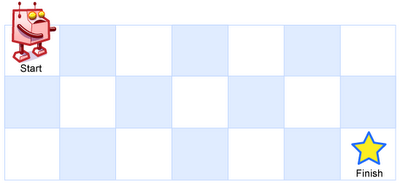
\includegraphics[width=300pt]{robot-maze.png}\\
\figcaption{Above is a $3 \times 7$ grid. How many possible unique paths are there?}\label{fig:unique-paths}
\end{center}

\textbf{Note}: $m$ and $n$ will be at most 100.


\subsection{深搜}
深搜,小集合可以过,大集合会超时

\subsubsection{代码}
\begin{Code}
// LeetCode, Unique Paths
// 深搜,小集合可以过,大集合会超时
class Solution {
public:
    int uniquePaths(int m, int n) {
        this->m = m;
        this->n = n;
        return uniquePathsRecursive(m, n);
    }
private:
    int m, n;

    int uniquePathsRecursive(int x, int y) {
        if (x < 1 || x > m) return 0; // 数据非法
        if (y < 1 || y > n) return 0;

        if (x == 1 && y == 1) return 1; // 终止条件

        return uniquePathsRecursive(x - 1, y) + uniquePathsRecursive(x, y - 1);
    }
};
\end{Code}


\subsection{备忘录法}
给前面的深搜,加个缓存,就可以过大集合了。即备忘录法。

\subsubsection{代码}
\begin{Code}
// LeetCode, Unique Paths
// 深搜 + 缓存,即备忘录法
class Solution {
public:
    int uniquePaths(int m, int n) {
        this->m = m;
        this->n = n;
        // 0行和0列未使用
        this->f = vector<vector<int> >(m + 1, vector<int>(n + 1, 0));
        return cachedUniquePathsRecursive(m, n);
    }
private:
    int m, n;  // 全局只读数据
    vector<vector<int> > f;  // 缓存

    int uniquePathsRecursive(int x, int y) {
        if (x < 1 || x > m) return 0; // 数据非法,终止条件
        if (y < 1 || y > n) return 0;

        if (x == 1 && y == 1) return 1; // 回到起点,收敛条件

        return cachedUniquePathsRecursive(x - 1, y) +
                cachedUniquePathsRecursive(x, y - 1);
    }

    int cachedUniquePathsRecursive(int x, int y) {
        if (f[x][y] > 0) return f[x][y];
        else return f[x][y] = uniquePathsRecursive(x, y);
    }
};
\end{Code}


\subsection{动规}
既然可以用备忘录法自顶向下解决,也一定可以用动规自底向上解决。

设状态为\fn{f[i][j]},表示从起点$(1,1)$到达$(i,j)$的路线条数,则状态转移方程为:
\begin{Code}
f[i][j]=f[i-1][j]+f[i][j-1]
\end{Code}


\subsubsection{代码}
\begin{Code}
// LeetCode, Unique Paths
// 动规,滚动数组
class Solution {
public:
    int uniquePaths(int m, int n) {
        vector<int> f(n, 0);
        f[0] = 1;
        for (int i = 0; i < m; i++) {
            for (int j = 1; j < n; j++) {
                // 左边的f[j],表示更新后的f[j],与公式中的f[i[[j]对应
                // 右边的f[j],表示老的f[j],与公式中的f[i-1][j]对应
                f[j] = f[j - 1] + f[j];
            }
        }
        return f[n - 1];
    }
};
\end{Code}


\subsection{数学公式}
一个$m$行,$n$列的矩阵,机器人从左上走到右下总共需要的步数是$m+n-2$,其中向下走的步数是$m-1$,因此问题变成了在$m+n-2$个操作中,选择$m–1$个时间点向下走,选择方式有多少种。即 $C_{m+n-2}^{m-1}$ 。

\subsubsection{代码}
\begin{Code}
// LeetCode, Unique Paths
// 数学公式
class Solution {
public:
    typedef long long int64_t;
    // 求阶乘, n!/(start-1)!,即 n*(n-1)...start,要求 n >= 1
    static int64_t factor(int n, int start = 1) {
        int64_t  ret = 1;
        for(int i = start; i <= n; ++i)
            ret *= i;
        return ret;
    }
    // 求组合数 C_n^k
    static int64_t combination(int n, int k) {
        // 常数优化
        if (k == 0) return 1;
        if (k == 1) return n;

        int64_t ret = factor(n, k+1);
        ret /= factor(n - k);
        return ret;
    }

    int uniquePaths(int m, int n) {
        // max 可以防止n和k差距过大,从而防止combination()溢出
        return combination(m+n-2, max(m-1, n-1));
    }
};
\end{Code}


\subsubsection{相关题目}
\begindot
\item Unique Paths II,见 \S \ref{sec:unique-paths-ii}
\myenddot


\section{Unique Paths II} %%%%%%%%%%%%%%%%%%%%%%%%%%%%%%
\label{sec:unique-paths-ii}


\subsubsection{描述}
Follow up for "Unique Paths":

Now consider if some obstacles are added to the grids. How many unique paths would there be?

An obstacle and empty space is marked as 1 and 0 respectively in the grid.

For example,

There is one obstacle in the middle of a $3 \times 3$ grid as illustrated below.
\begin{Code}
[
  [0,0,0],
  [0,1,0],
  [0,0,0]
]
\end{Code}

The total number of unique paths is 2.

Note: $m$ and $n$ will be at most 100.


\subsection{备忘录法}
在上一题的基础上改一下即可。相比动规,简单得多。

\subsubsection{代码}
\begin{Code}
// LeetCode, Unique Paths II
// 深搜 + 缓存,即备忘录法
class Solution {
public:
    int uniquePathsWithObstacles(vector<vector<int> > &obstacleGrid) {
        const int m = obstacleGrid.size();
        const int n = obstacleGrid[0].size();
        // 0行和0列未使用
        this->f = vector<vector<int> >(m + 1, vector<int>(n + 1, 0));
        return cachedUniquePathsRecursive(obstacleGrid, m, n);
    }
private:
    vector<vector<int> > f;  // 缓存

    int uniquePathsRecursive(const vector<vector<int> > &obstacleGrid,
            int x, int y) {
        if (x < 1 || x > obstacleGrid.size()) return 0; // 数据非法,终止条件
        if (y < 1 || y > obstacleGrid[0].size()) return 0;

        // (x,y)是障碍
        if (obstacleGrid[x-1][y-1]) return 0;

        if (x == 1 and y == 1) return 1; // 回到起点,收敛条件

        return cachedUniquePathsRecursive(obstacleGrid, x - 1, y) +
                cachedUniquePathsRecursive(obstacleGrid, x, y - 1);
    }

    int cachedUniquePathsRecursive(const vector<vector<int> > &obstacleGrid,
            int x, int y) {
        if (f[x][y] > 0) return f[x][y];
        else return f[x][y] = uniquePathsRecursive(obstacleGrid, x, y);
    }
};
\end{Code}


\subsection{动规}
与上一题类似,但要特别注意第一列的障碍。在上一题中,第一列全部是1,但是在这一题中不同,第一列如果某一行有障碍物,那么后面的行应该为0。


\subsubsection{代码}
\begin{Code}
// LeetCode, Unique Paths II
// 动规,滚动数组
class Solution {
public:
    int uniquePathsWithObstacles(vector<vector<int> > &obstacleGrid) {
        const int m = obstacleGrid.size();
        const int n = obstacleGrid[0].size();
        if (obstacleGrid[0][0] || obstacleGrid[m-1][n-1]) return 0;

        vector<int> f(n, 0);

        // 寻找第一列的第一个障碍在哪一行
        int first_col_obstacle = INT_MAX;
        for (int i = 0; i < m; i++) {
            if (obstacleGrid[i][0]) {
                first_col_obstacle = i;
                break;
            }
        }

        for (int i = 0; i < m; i++) {
            // 第一列如果某一行有障碍物,那么后面的行应该为0。
            if(i >= first_col_obstacle) f[0] = 0;
            else f[0] = 1;
            for (int j = 1; j < n; j++) {
                if (!obstacleGrid[i][j]) {
                    // 左边的f[j],表示更新后的f[j],与公式中的f[i[[j]对应
                    // 右边的f[j],表示老的f[j],与公式中的f[i-1][j]对应
                    f[j] = f[j - 1] + f[j];
                } else {
                    f[j] = 0;
                }
            }
        }
        return f[n - 1];
    }
};
\end{Code}


\subsubsection{相关题目}
\begindot
\item Unique Paths,见 \S \ref{sec:unique-paths}
\myenddot


\section{N-Queens} %%%%%%%%%%%%%%%%%%%%%%%%%%%%%%
\label{sec:n-queens}


\subsubsection{描述}
The \emph{n-queens puzzle} is the problem of placing n queens on an $n \times n$ chessboard such that no two queens attack each other.

\begin{center}
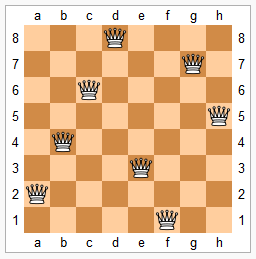
\includegraphics{8-queens.png}\\
\figcaption{Eight Queens}\label{fig:8-queens}
\end{center}

Given an integer $n$, return all distinct solutions to the n-queens puzzle.

Each solution contains a distinct board configuration of the n-queens' placement, where \fn{'Q'} and \fn{'.'} both indicate a queen and an empty space respectively.

For example,
There exist two distinct solutions to the 4-queens puzzle:
\begin{Code}
[
 [".Q..",  // Solution 1
  "...Q",
  "Q...",
  "..Q."],

 ["..Q.",  // Solution 2
  "Q...",
  "...Q",
  ".Q.."]
]
\end{Code}


\subsubsection{分析}
经典的深搜题。

\subsubsection{代码}
\begin{Code}
// LeetCode, N-Queens
// 深搜+剪枝
class Solution {
public:
    vector<vector<string> > solveNQueens(int n) {
        this->columns = vector<int>(n, 0);
        this->principal_diagonals = vector<int>(2 * n, 0);
        this->counter_diagonals = vector<int>(2 * n, 0);

        vector<vector<string> > result;
        vector<int> C(n, 0);  // C[i]表示第i行皇后所在的列编号
        solveNQueens(0, C, result);
        return result;
    }
private:
    // 这三个变量用于剪枝
    vector<int> columns;  // 表示已经放置的皇后占据了哪些列
    vector<int> principal_diagonals;  // 占据了哪些主对角线
    vector<int> counter_diagonals;  // 占据了哪些副对角线

    void solveNQueens(int row, vector<int> &C,
            vector<vector<string> > &result) {
        const int N = C.size();
        if (row == N) { // 终止条件,也是收敛条件,意味着找到了一个可行解
            vector<string> solution;
            for (int i = 0; i < N; ++i) {
                string s(N, '.');
                for (int j = 0; j < N; ++j) {
                    if (j == C[i]) s[j] = 'Q';
                }
                solution.push_back(s);
            }
            result.push_back(solution);
            return;
        }

        for (int j = 0; j < N; ++j) {  // 扩展状态,一列一列的试
            const bool ok = columns[j] == 0 &&
                    principal_diagonals[row + j] == 0
                    && counter_diagonals[row - j + N] == 0;
            if (ok) {  // 剪枝:如果合法,继续递归
                // 执行扩展动作
                C[row] = j;
                columns[j] = principal_diagonals[row + j] =
                        counter_diagonals[row - j + N] = 1;
                solveNQueens(row + 1, C, result);
                // 撤销动作
                // C[row] = 0;
                columns[j] = principal_diagonals[row + j] =
                        counter_diagonals[row - j + N] = 0;
            }
        }
    }
};
\end{Code}


\subsubsection{相关题目}
\begindot
\item N-Queens II,见 \S \ref{sec:n-queens-ii}
\myenddot


\section{N-Queens II} %%%%%%%%%%%%%%%%%%%%%%%%%%%%%%
\label{sec:n-queens-ii}


\subsubsection{描述}
Follow up for N-Queens problem.

Now, instead outputting board configurations, return the total number of distinct solutions.


\subsubsection{分析}
只需要输出解的个数,不需要输出所有解,代码要比上一题简化很多。设一个全局计数器,每找到一个解就增1。


\subsubsection{代码}
\begin{Code}
// LeetCode, N-Queens II
// 深搜+剪枝
class Solution {
public:
    int totalNQueens(int n) {
        this->count = 0;
        this->columns = vector<int>(n, 0);
        this->principal_diagonals = vector<int>(2 * n, 0);
        this->counter_diagonals = vector<int>(2 * n, 0);

        vector<vector<string> > result;
        vector<int> C(n, 0);  // C[i]表示第i行皇后所在的列编号
        solveNQueens(0, C, result);
        return this->count;
    }
private:
    int count; // 解的个数
    // 这三个变量用于剪枝
    vector<int> columns;  // 表示已经放置的皇后占据了哪些列
    vector<int> principal_diagonals;  // 占据了哪些主对角线
    vector<int> counter_diagonals;  // 占据了哪些副对角线

    void solveNQueens(int row, vector<int> &C,
            vector<vector<string> > &result) {
        const int N = C.size();
        if (row == N) { // 终止条件,也是收敛条件,意味着找到了一个可行解
            this->count++;
            return;
        }

        for (int j = 0; j < N; ++j) {  // 扩展状态,一列一列的试
            const bool ok = columns[j] == 0 &&
                    principal_diagonals[row + j] == 0
                    && counter_diagonals[row - j + N] == 0;
            if (ok) {  // 剪枝:如果合法,继续递归
                // 执行扩展动作
                C[row] = j;
                columns[j] = principal_diagonals[row + j] =
                        counter_diagonals[row - j + N] = 1;
                solveNQueens(row + 1, C, result);
                // 撤销动作
                // C[row] = 0;
                columns[j] = principal_diagonals[row + j] =
                        counter_diagonals[row - j + N] = 0;
            }
        }
    }
};
\end{Code}


\subsubsection{相关题目}
\begindot
\item N-Queens,见 \S \ref{sec:n-queens}
\myenddot


\section{Restore IP Addresses} %%%%%%%%%%%%%%%%%%%%%%%%%%%%%%
\label{sec:restore-ip-addresses}


\subsubsection{描述}
Given a string containing only digits, restore it by returning all possible valid IP address combinations.

For example:
Given \code{"25525511135"},

return \code{["255.255.11.135", "255.255.111.35"]}. (Order does not matter)


\subsubsection{分析}
必须要走到底部才能判断解是否合法,深搜。


\subsubsection{代码}
\begin{Code}
// LeetCode, Restore IP Addresses
class Solution {
public:
    vector<string> restoreIpAddresses(string s) {
        vector<string> result;
        string ip; // 存放中间结果
        dfs(s, 0, 0, ip, result);
        return result;
    }

    /**
     * @brief 解析字符串
     * @param[in] s 字符串,输入数据
     * @param[in] startIndex 从s的哪里开始
     * @param[in] step 当前步骤编号,从0开始编号,取值为0,1,2,3,4表示结束了
     * @param[out] intermediate 当前解析出来的中间结果
     * @param[out] result 存放所有可能的IP地址
     * @return 无
     */
    void dfs(string s, int start, int step, string ip,
            vector<string> &result) {
        if (s.size() - start > (4 - step) * 3)
            return;  // 非法结果,剪枝
        if (s.size() - start < (4 - step))
            return;  // 非法结果,剪枝

        if (start == s.size() && step == 4) {  // 找到一个合法解
            ip.resize(ip.size() - 1);
            result.push_back(ip);
            return;
        }

        int num = 0;
        for (int i = start; i < start + 3; i++) {
            num = num * 10 + (s[i] - '0');

            if (num <= 255) {  // 当前结点合法,则继续往下递归
                ip += s[i];
                dfs(s, i + 1, step + 1, ip + '.', result);
            }
            if (num == 0) break;  // 不允许前缀0,但允许单个0
        }
    }
};
\end{Code}


\subsubsection{相关题目}
\begindot
\item 无
\myenddot


\section{Combination Sum} %%%%%%%%%%%%%%%%%%%%%%%%%%%%%%
\label{sec:combination-sum}


\subsubsection{描述}
Given a set of candidate numbers ($C$) and a target number ($T$), find all unique combinations in $C$ where the candidate numbers sums to $T$.

The same repeated number may be chosen from $C$ \emph{unlimited} number of times.

Note:
\begindot
\item All numbers (including target) will be positive integers.
\item Elements in a combination ($a_1, a_2, ..., a_k$) must be in non-descending order. (ie, $a_1 > a_2 > ... > a_k$).
\item The solution set must not contain duplicate combinations.
\myenddot

For example, given candidate set \fn{2,3,6,7} and target \fn{7}, 
A solution set is: 
\begin{Code}
[7] 
[2, 2, 3] 
\end{Code}


\subsubsection{分析}
无


\subsubsection{代码}
\begin{Code}
// LeetCode, Combination Sum
class Solution {
public:
    vector<vector<int> > combinationSum(vector<int> &nums, int target) {
        std::sort(nums.begin(), nums.end());
        vector<vector<int> > result; // 最终结果
        vector<int> intermediate; // 中间结果
        dfs(nums, target, 0, intermediate, result);
        return result;
    }

private:
    void dfs(vector<int>& nums, int gap, int level, vector<int>& intermediate,
            vector<vector<int> > &result) {
        if (gap == 0) {  // 找到一个合法解
            result.push_back(intermediate);
            return;
        }
        for (size_t i = level; i < nums.size(); i++) { // 扩展状态
            if (gap < nums[i]) return; // 剪枝

            intermediate.push_back(nums[i]); // 执行扩展动作
            dfs(nums, gap - nums[i], i, intermediate, result);
            intermediate.pop_back();  // 撤销动作
        }
    }
};
\end{Code}


\subsubsection{相关题目}
\begindot
\item Combination Sum II ,见 \S \ref{sec:combination-sum-ii}
\myenddot


\section{Combination Sum II} %%%%%%%%%%%%%%%%%%%%%%%%%%%%%%
\label{sec:combination-sum-ii}


\subsubsection{描述}
Given a set of candidate numbers ($C$) and a target number ($T$), find all unique combinations in $C$ where the candidate numbers sums to $T$.

The same repeated number may be chosen from $C$ \emph{once} number of times.

Note:
\begindot
\item All numbers (including target) will be positive integers.
\item Elements in a combination ($a_1, a_2, ..., a_k$) must be in non-descending order. (ie, $a_1 > a_2 > ... > a_k$).
\item The solution set must not contain duplicate combinations.
\myenddot

For example, given candidate set \fn{10,1,2,7,6,1,5} and target \fn{8}, 
A solution set is: 
\begin{Code}
[1, 7] 
[1, 2, 5] 
[2, 6] 
[1, 1, 6]
\end{Code}


\subsubsection{分析}
无


\subsubsection{代码}
\begin{Code}
// LeetCode, Combination Sum II
class Solution {
public:
    vector<vector<int> > combinationSum2(vector<int> &nums, int target) {
        std::sort(nums.begin(), nums.end()); // 跟第 50 行配合,
                                             // 确保每个元素最多只用一次
        vector<vector<int> > result;
        vector<int> intermediate;
        dfs(nums, target, 0, intermediate, result);
        return result;
    }
private:
    // 使用nums[index, nums.size())之间的元素,能找到的所有可行解
    static void dfs(vector<int> &nums, int gap, int index,
            vector<int> &intermediate, vector<vector<int> > &result) {
        if (gap == 0) {  //  找到一个合法解
            result.push_back(intermediate);
            return;
        }

        int previous = -1;
        for (size_t i = index; i < nums.size(); i++) {
            // 如果上一轮循环没有选nums[i],则本次循环就不能再选nums[i],
            // 确保nums[i]最多只用一次
            if (previous == nums[i]) continue;

            if (gap < nums[i]) return;  // 剪枝

            previous = nums[i];

            intermediate.push_back(nums[i]);
            dfs(nums, gap - nums[i], i + 1, intermediate, result);
            intermediate.pop_back();  // 恢复环境
        }
    }
};
\end{Code}


\subsubsection{相关题目}
\begindot
\item Combination Sum ,见 \S \ref{sec:combination-sum}
\myenddot

\chapter{细节实现题}
这类题目不考特定的算法,纯粹考察写代码的熟练度。


\section{Reverse Integer (loj7)} %%%%%%%%%%%%%%%%%%%%%%%%%%%%%%
\label{sec:reverse-integer}


\subsubsection{描述}
Reverse digits of an integer.

Example1: x = 123, return 321

Example2: x = -123, return -321


\textbf{Have you thought about this?}

Here are some good questions to ask before coding. Bonus points for you if you have already thought through this!

If the integer's last digit is 0, what should the output be? ie, cases such as 10, 100.

Did you notice that the reversed integer might overflow? Assume the input is a 32-bit integer, then the reverse of 1000000003 overflows. How should you handle such cases?

For the purpose of this problem, assume that your function returns 0 when the reversed integer overflows.

Update (2014-11-10):

Test cases had been added to test the overflow behavior.

\subsubsection{分析}
短小精悍的题,代码也可以写的很短小。


\subsubsection{代码}
\begin{Code}
// LeetCode, Reverse Integer
// 时间复杂度O(logn),空间复杂度O(1)
class Solution {
public:
    int reverse (int x) {
        int r = 0;

        while(x!=0) {
            if(r > INT_MAX/10 || r < INT_MIN/10) {
                return 0;
            }
            r = r * 10 + x % 10;
            x /= 10;
        }
        
        return r;
    }
};
\end{Code}

\subsubsection{代码}
\begin{Code}
// LeetCode, Reverse Integer
// 使用绝对值再判断符号
class Solution {
public:
int reverse(int x) {
        unsigned int val = abs(x);
        unsigned int result = 0;

        while (val) {
            if (result > ((unsigned int)(1 << 31) - 1) / 10)
                return 0;

            result = result * 10 + val % 10;
            val /= 10;
        }

        return (x > 0 ? result : (-1 * result));
    }
};
\end{Code}

\subsubsection{代码}
\begin{Code}
// LeetCode, Reverse Integer
// 使用long
class Solution {
public:
    int reverse(int x) {
        long long ret = 0;
        while (x) {
            int data = x % 10;
            ret = ret * 10 + data;
            if (ret > numeric_limits<int>::max() || ret <= numeric_limits<int>::min()) {
                ret = 0;
                break;
            }
            x /= 10;
        }
        return ret;
    }
};
\end{Code}

\subsubsection{代码}
\begin{Code}
// 不使用long判断溢出
class Solution {
public:
    int reverse(int x) {
        if(x==INT_MIN)
        //solve this situation, we can use x=abs(x)
            return 0;
        int isPositive=1;
        if(x<0)
        {
            x=abs(x);
            isPositive=-1;
        }
        int result=0;
        int int_maxp=INT_MAX/10;
        while(x!=0)
        {
            if (result>int_maxp)
            // don't need to check "result == int_maxp && q > int_maxq"
            // because this can't happen (x is type int)
            {
                result=0;
                break;
            }
            else
                result=10*result+x%10;
            x=x/10;
        }
        result=isPositive*result;
        return result;
    }
};
\end{Code}

\subsubsection{相关题目}
\begindot
\item Palindrome Number, 见 \S \ref{sec:palindrome-number}
\myenddot


\section{Palindrome Number (loj9)} %%%%%%%%%%%%%%%%%%%%%%%%%%%%%%
\label{sec:palindrome-number}


\subsubsection{描述}
Determine whether an integer is a palindrome. Do this without extra space.

\textbf{Some hints:}

Could negative integers be palindromes? (ie, -1)

If you are thinking of converting the integer to string, note the restriction of using extra space.

You could also try reversing an integer. However, if you have solved the problem "Reverse Integer", you know that the reversed integer might overflow. How would you handle such case?

There is a more generic way of solving this problem.


\subsubsection{分析}
首先想到,可以利用上一题,将整数反转,然后与原来的整数比较,是否相等,相等则为 Palindrome 的。可是 reverse()会溢出。

正确的解法是,不断地取第一位和最后一位(10进制下)进行比较,相等则取第二位和倒数第二位,直到完成比较或者中途找到了不一致的位。


\subsubsection{代码}
\begin{Code}
//LeetCode, Palindrome Number
// 时间复杂度O(1),空间复杂度O(1)
class Solution {
public:
    bool isPalindrome(int x) {
        if (x < 0) return false;
        int d = 1; // divisor
        while (x / d >= 10) d *= 10;

        while (x > 0) {
            int q = x / d;  // quotient
            int r = x % 10;   // remainder
            if (q != r) return false;
            // remove the highest bit and remove the lowest bit
            x = x % d / 10;
            d /= 100;
        }
        return true;
    }
};
\end{Code}


\subsubsection{相关题目}
\begindot
\item Reverse Integer, 见 \S \ref{sec:reverse-integer}
\item Valid Palindrome, 见 \S \ref{sec:valid-palindrome}
\myenddot


\section{Insert Interval} %%%%%%%%%%%%%%%%%%%%%%%%%%%%%%
\label{sec:insert-interval}


\subsubsection{描述}
Given a set of non-overlapping intervals, insert a new interval into the intervals (merge if necessary).

You may assume that the intervals were initially sorted according to their start times.

Example 1:
Given intervals \code{[1,3],[6,9]}, insert and merge \code{[2,5]} in as \code{[1,5],[6,9]}.

Example 2:
Given \code{[1,2],[3,5],[6,7],[8,10],[12,16]}, insert and merge \code{[4,9]} in as \code{[1,2],[3,10],[12,16]}.

This is because the new interval \code{[4,9]} overlaps with \code{[3,5],[6,7],[8,10]}.


\subsubsection{分析}
无


\subsubsection{代码}
\begin{Code}
struct Interval {
    int start;
    int end;
    Interval() : start(0), end(0) { }
    Interval(int s, int e) : start(s), end(e) { }
};
 
//LeetCode, Insert Interval
// 时间复杂度O(n),空间复杂度O(1)
class Solution {
public:
    vector<Interval> insert(vector<Interval> &intervals, Interval newInterval) {
        vector<Interval>::iterator it = intervals.begin();
        while (it != intervals.end()) {
            if (newInterval.end < it->start) {
                intervals.insert(it, newInterval);
                return intervals;
            } else if (newInterval.start > it->end) {
                it++;
                continue;
            } else {
                newInterval.start = min(newInterval.start, it->start);
                newInterval.end = max(newInterval.end, it->end);
                it = intervals.erase(it);
            }
        }
        intervals.insert(intervals.end(), newInterval);
        return intervals;
    }
};
\end{Code}


\subsubsection{相关题目}

\begindot
\item Merge Intervals,见 \S \ref{sec:merge-intervals}
\myenddot


\section{Merge Intervals} %%%%%%%%%%%%%%%%%%%%%%%%%%%%%%
\label{sec:merge-intervals}


\subsubsection{描述}
Given a collection of intervals, merge all overlapping intervals.

For example,
Given \code{[1,3],[2,6],[8,10],[15,18]},
return \code{[1,6],[8,10],[15,18]}


\subsubsection{分析}
复用一下Insert Intervals的解法即可,创建一个新的interval集合,然后每次从旧的里面取一个interval出来,然后插入到新的集合中。


\subsubsection{代码}
\begin{Code}
struct Interval {
    int start;
    int end;
    Interval() : start(0), end(0) { }
    Interval(int s, int e) : start(s), end(e) { }
};
 
//LeetCode, Merge Interval
//复用一下Insert Intervals的解法即可
// 时间复杂度O(n1+n2+...),空间复杂度O(1)
class Solution {
public:
    vector<Interval> merge(vector<Interval> &intervals) {
        vector<Interval> result;
        for (int i = 0; i < intervals.size(); i++) {
            insert(result, intervals[i]);
        }
        return result;
    }
private:
    vector<Interval> insert(vector<Interval> &intervals, Interval newInterval) {
        vector<Interval>::iterator it = intervals.begin();
        while (it != intervals.end()) {
            if (newInterval.end < it->start) {
                intervals.insert(it, newInterval);
                return intervals;
            } else if (newInterval.start > it->end) {
                it++;
                continue;
            } else {
                newInterval.start = min(newInterval.start, it->start);
                newInterval.end = max(newInterval.end, it->end);
                it = intervals.erase(it);
            }
        }
        intervals.insert(intervals.end(), newInterval);
        return intervals;
    }
};
\end{Code}


\subsubsection{相关题目}

\begindot
\item Insert Interval,见 \S \ref{sec:insert-interval}
\myenddot


\section{Minimum Window Substring} %%%%%%%%%%%%%%%%%%%%%%%%%%%%%%
\label{sec:minimum-window-substring}


\subsubsection{描述}
Given a string $S$ and a string $T$, find the minimum window in $S$ which will contain all the characters in $T$ in complexity $O(n)$.

For example, \code{S = "ADOBECODEBANC", T = "ABC"}

Minimum window is \code{"BANC"}.

Note:
\begindot
\item If there is no such window in $S$ that covers all characters in $T$, return the emtpy string \code{""}.
\item If there are multiple such windows, you are guaranteed that there will always be only one unique minimum window in $S$.
\myenddot


\subsubsection{分析}
双指针,动态维护一个区间。尾指针不断往后扫,当扫到有一个窗口包含了所有$T$的字符后,然后再收缩头指针,直到不能再收缩为止。最后记录所有可能的情况中窗口最小的


\subsubsection{代码}
\begin{Code}
// LeetCode, Minimum Window Substring
// 时间复杂度O(n),空间复杂度O(1)
class Solution {
public:
    string minWindow(string S, string T) {
        if (S.empty()) return "";
        if (S.size() < T.size()) return "";

        const int ASCII_MAX = 256;
        int appeared_count[ASCII_MAX];
        int expected_count[ASCII_MAX];
        fill(appeared_count, appeared_count + ASCII_MAX, 0);
        fill(expected_count, expected_count + ASCII_MAX, 0);

        for (size_t i = 0; i < T.size(); i++) expected_count[T[i]]++;

        int minWidth = INT_MAX, min_start = 0;  // 窗口大小,起点
        int wnd_start = 0;
        int appeared = 0;  // 完整包含了一个T
        //尾指针不断往后扫
        for (size_t wnd_end = 0; wnd_end < S.size(); wnd_end++) {
            if (expected_count[S[wnd_end]] > 0)  {  // this char is a part of T
                appeared_count[S[wnd_end]]++;
                if (appeared_count[S[wnd_end]] <= expected_count[S[wnd_end]])
                    appeared++;
            }
            if (appeared == T.size()) {  // 完整包含了一个T
                // 收缩头指针
                while (appeared_count[S[wnd_start]] > expected_count[S[wnd_start]]
                        || expected_count[S[wnd_start]] == 0) {
                    appeared_count[S[wnd_start]]--;
                    wnd_start++;
                }
                if (minWidth > (wnd_end - wnd_start + 1)) {
                    minWidth = wnd_end - wnd_start + 1;
                    min_start = wnd_start;
                }
            }
        }

        if (minWidth == INT_MAX) return "";
        else return S.substr(min_start, minWidth);
    }
};
\end{Code}


\subsubsection{相关题目}

\begindot
\item 无
\myenddot


\section{Multiply Strings} %%%%%%%%%%%%%%%%%%%%%%%%%%%%%%
\label{sec:multiply-strings}


\subsubsection{描述}
Given two numbers represented as strings, return multiplication of the numbers as a string.

Note: The numbers can be arbitrarily large and are non-negative.


\subsubsection{分析}
高精度乘法。

常见的做法是将字符转化为一个int,一一对应,形成一个int数组。但是这样很浪费空间,一个int32的最大值是$2^{31}-1=2147483647$,可以与9个字符对应,由于有乘法,减半,则至少可以与4个字符一一对应。一个int64可以与9个字符对应。


\subsubsection{代码1}
\begin{Code}
// LeetCode, Multiply Strings
// @author 连城 (http://weibo.com/lianchengzju)
// 一个字符对应一个int
// 时间复杂度O(n*m),空间复杂度O(n+m)
typedef vector<int> bigint;

bigint make_bigint(string const& repr) {
    bigint n;
    transform(repr.rbegin(), repr.rend(), back_inserter(n),
            [](char c) { return c - '0'; });
    return n;
}

string to_string(bigint const& n) {
    string str;
    transform(find_if(n.rbegin(), prev(n.rend()),
            [](char c) { return c > '\0'; }), n.rend(), back_inserter(str),
            [](char c) { return c + '0'; });
    return str;
}

bigint operator*(bigint const& x, bigint const& y) {
    bigint z(x.size() + y.size());

    for (size_t i = 0; i < x.size(); ++i)
        for (size_t j = 0; j < y.size(); ++j) {
            z[i + j] += x[i] * y[j];
            z[i + j + 1] += z[i + j] / 10;
            z[i + j] %= 10;
        }

    return z;
}

class Solution {
public:
    string multiply(string num1, string num2) {
        return to_string(make_bigint(num1) * make_bigint(num2));
    }
};
\end{Code}


\subsubsection{代码2}
\begin{Code}
// LeetCode, Multiply Strings
// 9个字符对应一个int64_t
// 时间复杂度O(n*m/81),空间复杂度O((n+m)/9)
/** 大整数类. */
class BigInt {
public:
    /**
     * @brief 构造函数,将字符串转化为大整数.
     * @param[in] s 输入的字符串
     * @return 无
     */
    BigInt(string s) {
        vector<int64_t> result;
        result.reserve(s.size() / RADIX_LEN + 1);

        for (int i = s.size(); i > 0; i -= RADIX_LEN) {  // [i-RADIX_LEN, i)
            int temp = 0;
            const int low = max(i - RADIX_LEN, 0);
            for (int j = low; j < i; j++) {
                temp = temp * 10 + s[j] - '0';
            }
            result.push_back(temp);
        }
        elems = result;
    }
    /**
     * @brief 将整数转化为字符串.
     * @return 字符串
     */
    string toString() {
        stringstream result;
        bool started = false; // 用于跳过前导0
        for (auto i = elems.rbegin(); i != elems.rend(); i++) {
            if (started) { // 如果多余的0已经都跳过,则输出
                result << setw(RADIX_LEN) << setfill('0') << *i;
            } else {
                result << *i;
                started = true; // 碰到第一个非0的值,就说明多余的0已经都跳过
            }
        }

        if (!started) return "0"; // 当x全为0时
        else return result.str();
    }

    /**
     * @brief 大整数乘法.
     * @param[in] x x
     * @param[in] y y
     * @return 大整数
     */
    static BigInt multiply(const BigInt &x, const BigInt &y) {
        vector<int64_t> z(x.elems.size() + y.elems.size(), 0);

        for (size_t i = 0; i < y.elems.size(); i++) {
            for (size_t j = 0; j < x.elems.size(); j++) { // 用y[i]去乘以x的各位
                //  两数第i, j位相乘,累加到结果的第i+j位
                z[i + j] += y.elems[i] * x.elems[j];

                if (z[i + j] >= BIGINT_RADIX) { //  看是否要进位
                    z[i + j + 1] += z[i + j] / BIGINT_RADIX; //  进位
                    z[i + j] %= BIGINT_RADIX;
                }
            }
        }
        while (z.back() == 0) z.pop_back();  // 没有进位,去掉最高位的0
        return BigInt(z);
    }

private:
    typedef long long int64_t;
    /** 一个数组元素对应9个十进制位,即数组是亿进制的
     * 因为 1000000000 * 1000000000 没有超过 2^63-1
     */
    const static int BIGINT_RADIX = 1000000000;
    const static int RADIX_LEN = 9;
    /** 万进制整数. */
    vector<int64_t> elems;
    BigInt(const vector<int64_t> num) : elems(num) {}
};


class Solution {
public:
    string multiply(string num1, string num2) {
        BigInt x(num1);
        BigInt y(num2);
        return BigInt::multiply(x, y).toString();
    }
};
\end{Code}


\subsubsection{相关题目}

\begindot
\item 无
\myenddot


\section{Substring with Concatenation of All Words} %%%%%%%%%%%%%%%%%%%%%%%%%%%%%%
\label{sec:substring-with-concatenation-of-all-words}


\subsubsection{描述}
You are given a string, $S$, and a list of words, $L$, that are all of the same length. Find all starting indices of substring(s) in $S$ that is a concatenation of each word in $L$ exactly once and without any intervening characters.

For example, given: 
\begin{Code}
S: "barfoothefoobarman"
L: ["foo", "bar"]
\end{Code}

You should return the indices: \code{[0,9]}.(order does not matter).


\subsubsection{分析}
无


\subsubsection{代码}
\begin{Code}
// LeetCode, Substring with Concatenation of All Words
// 时间复杂度O(n*m),空间复杂度O(m)
class Solution {
public:
    vector<int> findSubstring(string s, vector<string>& dict) {
        size_t wordLength = dict.front().length();
        size_t catLength = wordLength * dict.size();
        vector<int> result;

        if (s.length() < catLength) return result;

        unordered_map<string, int> wordCount;

        for (auto const& word : dict) ++wordCount[word];

        for (auto i = begin(s); i <= prev(end(s), catLength); ++i) {
            unordered_map<string, int> unused(wordCount);

            for (auto j = i; j != next(i, catLength); j += wordLength) {
                auto pos = unused.find(string(j, next(j, wordLength)));

                if (pos == unused.end() || pos->second == 0) break;

                if (--pos->second == 0) unused.erase(pos);
            }

            if (unused.size() == 0) result.push_back(distance(begin(s), i));
        }

        return result;
    }
};
\end{Code}


\subsubsection{相关题目}

\begindot
\item 无
\myenddot


\section{Pascal's Triangle (loj118)} %%%%%%%%%%%%%%%%%%%%%%%%%%%%%%
\label{sec:pascals-triangle}


\subsubsection{描述}
Given $numRows$, generate the first $numRows$ of Pascal's triangle.

For example, given $numRows = 5$,

Return
\begin{Code}
[
     [1],
    [1,1],
   [1,2,1],
  [1,3,3,1],
 [1,4,6,4,1]
]
\end{Code}


\subsubsection{分析}
本题可以用队列,计算下一行时,给上一行左右各加一个0,然后下一行的每个元素,就等于左上角和右上角之和。

另一种思路,下一行第一个元素和最后一个元素赋值为1,中间的每个元素,等于上一行的左上角和右上角元素之和。

\subsubsection{从左到右}
\begin{Code}
// LeetCode, Pascal's Triangle
// 时间复杂度O(n^2),空间复杂度O(n)
class Solution {
public:
    vector<vector<int>> generate(int numRows) {
        vector<vector<int>> result;
        if(numRows == 0) return result;

        result.push_back(vector<int>(1,1)); //first row

        for(int i = 2; i <= numRows; ++i) {
            vector<int> current(i,1);  // 本行
            const vector<int> &prev = result[i-2];  // 上一行

            for(int j = 1; j < i - 1; ++j) {
                current[j] = prev[j-1] + prev[j]; // 左上角和右上角之和
            }
            result.push_back(current);
        }
        return result;
    }
};
\end{Code}

\subsubsection{从左到右}
\begin{Code}
class Solution {
public:
    vector<vector<int>> generate(int numRows) {
        vector<vector<int>> r(numRows);
        for (int i = 0; i < numRows; i++) {
            r[i].resize(i + 1);
            r[i][0] = r[i][i] = 1;
            for (int j = 1; j < i; j++)
                r[i][j] = r[i - 1][j - 1] + r[i - 1][j];
        }
        return r;
    }
};
\end{Code}

\subsubsection{从右到左}
\begin{Code}
// LeetCode, Pascal's Triangle
// 时间复杂度O(n^2),空间复杂度O(n)
class Solution {
public:
    vector<vector<int> > generate(int numRows) {
        vector<vector<int> > result;
        vector<int> array;
        for (int i = 1; i <= numRows; i++) {
            for (int j = i - 2; j > 0; j--) {
                array[j] = array[j - 1] + array[j];
            }
            array.push_back(1);
            result.push_back(array);
        }
        return result;
    }
};
\end{Code}


\subsubsection{相关题目}
\begindot
\item Pascal's Triangle II,见 \S \ref{sec:pascals-triangle-ii}
\myenddot


\section{Pascal's Triangle II} %%%%%%%%%%%%%%%%%%%%%%%%%%%%%%
\label{sec:pascals-triangle-ii}


\subsubsection{描述}
Given an index $k$, return the $k^{th}$ row of the Pascal's triangle.

For example, given $k = 3$,

Return \code{[1,3,3,1]}.

Note: Could you optimize your algorithm to use only $O(k)$ extra space?


\subsubsection{分析}
滚动数组。


\subsubsection{代码}

\begin{Code}
// LeetCode, Pascal's Triangle II
// 滚动数组,时间复杂度O(n^2),空间复杂度O(n)
class Solution {
public:
	vector<int> getRow(int rowIndex) {
		vector<int> array;
		for (int i = 0; i <= rowIndex; i++) {
			for (int j = i - 1; j > 0; j--){
				array[j] = array[j - 1] + array[j];
			}
			array.push_back(1);
		}
		return array;
	}
};
\end{Code}


\subsubsection{相关题目}
\begindot
\item Pascal's Triangle,见 \S \ref{sec:pascals-triangle}
\myenddot


\section{Spiral Matrix} %%%%%%%%%%%%%%%%%%%%%%%%%%%%%%
\label{sec:spiral-matrix}


\subsubsection{描述}
Given a matrix of $m \times n$ elements ($m$ rows, $n$ columns), return all elements of the matrix in spiral order.

For example,
Given the following matrix:
\begin{Code}
[
 [ 1, 2, 3 ],
 [ 4, 5, 6 ],
 [ 7, 8, 9 ]
]
\end{Code}
You should return \fn{[1,2,3,6,9,8,7,4,5]}.


\subsubsection{分析}
模拟。

\subsubsection{代码}
\begin{Code}
// LeetCode, Spiral Matrix
// @author 龚陆安 (http://weibo.com/luangong)
// 时间复杂度O(n^2),空间复杂度O(1)
class Solution {
public:
    vector<int> spiralOrder(vector<vector<int> >& matrix) {
        vector<int> result;
        if (matrix.empty()) return result;
        int beginX = 0, endX = matrix[0].size() - 1;
        int beginY = 0, endY = matrix.size() - 1;
        while (true) {
            // From left to right
            for (int j = beginX; j <= endX; ++j) result.push_back(matrix[beginY][j]);
            if (++beginY > endY) break;
            // From top to bottom
            for (int i = beginY; i <= endY; ++i) result.push_back(matrix[i][endX]);
            if (beginX > --endX) break;
            // From right to left
            for (int j = endX; j >= beginX; --j) result.push_back(matrix[endY][j]);
            if (beginY > --endY) break;
            // From bottom to top
            for (int i = endY; i >= beginY; --i) result.push_back(matrix[i][beginX]);
            if (++beginX > endX) break;
        }
        return result;
    }
};
\end{Code}


\subsubsection{相关题目}
\begindot
\item Spiral Matrix II ,见 \S \ref{sec:spiral-matrix-ii}
\myenddot


\section{Spiral Matrix II} %%%%%%%%%%%%%%%%%%%%%%%%%%%%%%
\label{sec:spiral-matrix-ii}


\subsubsection{描述}
Given an integer $n$, generate a square matrix filled with elements from 1 to $n^2$ in spiral order.

For example,
Given $n = 3$,

You should return the following matrix:
\begin{Code}
[
 [ 1, 2, 3 ],
 [ 8, 9, 4 ],
 [ 7, 6, 5 ]
]
\end{Code}


\subsubsection{分析}
这题比上一题要简单。


\subsubsection{代码1}
\begin{Code}
// LeetCode, Spiral Matrix II
// 时间复杂度O(n^2),空间复杂度O(n^2)
class Solution {
public:
    vector<vector<int> > generateMatrix(int n) {
        vector<vector<int> > matrix(n, vector<int>(n));
        int begin = 0, end = n - 1;
        int num = 1;

        while (begin < end) {
            for (int j = begin; j < end; ++j) matrix[begin][j] = num++;
            for (int i = begin; i < end; ++i) matrix[i][end] = num++;
            for (int j = end; j > begin; --j) matrix[end][j] = num++;
            for (int i = end; i > begin; --i) matrix[i][begin] = num++;
            ++begin;
            --end;
        }

        if (begin == end) matrix[begin][begin] = num;

        return matrix;
    }
};
\end{Code}


\subsubsection{代码2}
\begin{Code}
// LeetCode, Spiral Matrix II
// @author 龚陆安 (http://weibo.com/luangong)
// 时间复杂度O(n^2),空间复杂度O(n^2)
class Solution {
public:
    vector<vector<int> > generateMatrix(int n) {
        vector< vector<int> > matrix(n, vector<int>(n));
        if (n == 0) return matrix;
        int beginX = 0, endX = n - 1;
        int beginY = 0, endY = n - 1;
        int num = 1;
        while (true) {
            for (int j = beginX; j <= endX; ++j) matrix[beginY][j] = num++;
            if (++beginY > endY) break;

            for (int i = beginY; i <= endY; ++i) matrix[i][endX] = num++;
            if (beginX > --endX) break;

            for (int j = endX; j >= beginX; --j) matrix[endY][j] = num++;
            if (beginY > --endY) break;

            for (int i = endY; i >= beginY; --i) matrix[i][beginX] = num++;
            if (++beginX > endX) break;
        }
        return matrix;
    }
};
\end{Code}


\subsubsection{相关题目}
\begindot
\item Spiral Matrix, 见 \S \ref{sec:spiral-matrix}
\myenddot


\section{ZigZag Conversion} %%%%%%%%%%%%%%%%%%%%%%%%%%%%%%
\label{sec:zigzag-conversion}


\subsubsection{描述}
The string \code{"PAYPALISHIRING"} is written in a zigzag pattern on a given number of rows like this: (you may want to display this pattern in a fixed font for better legibility)

\begin{Code}
P   A   H   N
A P L S I I G
Y   I   R
\end{Code}

And then read line by line: \code{"PAHNAPLSIIGYIR"}

Write the code that will take a string and make this conversion given a number of rows:
\begin{Code}
string convert(string text, int nRows);
\end{Code}
\code{convert("PAYPALISHIRING", 3)} should return \code{"PAHNAPLSIIGYIR"}.


\subsubsection{分析}
要找到数学规律。真正面试中,不大可能出这种问题。

n=4:
\begin{Code}
P     I     N
A   L S   I G
Y A   H R
P     I
\end{Code}

n=5:
\begin{Code}
P       H
A     S I
Y   I   R
P L     I  G
A       N
\end{Code}

所以,对于每一层垂直元素的坐标 $(i,j)= (j+1 )*n +i$;对于每两层垂直元素之间的插入元素(斜对角元素),$(i,j)= (j+1)*n -i$


\subsubsection{代码}
\begin{Code}
// LeetCode, ZigZag Conversion
// 时间复杂度O(n),空间复杂度O(1)
class Solution {
public:
    string convert(string s, int nRows) {
        if (nRows <= 1 || s.size() <= 1) return s;
        string result;
        for (int i = 0; i < nRows; i++) {
            for (int j = 0, index = i; index < s.size();
                    j++, index = (2 * nRows - 2) * j + i) {
                result.append(1, s[index]);  // 垂直元素
                if (i == 0 || i == nRows - 1) continue;   // 斜对角元素
                if (index + (nRows - i - 1) * 2 < s.size())
                    result.append(1, s[index + (nRows - i - 1) * 2]);
            }
        }
        return result;
    }
};
\end{Code}


\subsubsection{相关题目}
\begindot
\item 无
\myenddot


\section{Divide Two Integers} %%%%%%%%%%%%%%%%%%%%%%%%%%%%%%
\label{sec:divide-two-integers}


\subsubsection{描述}
Divide two integers without using multiplication, division and mod operator.


\subsubsection{分析}
不能用乘、除和取模,那剩下的,还有加、减和位运算。

最简单的方法,是不断减去被除数。在这个基础上,可以做一点优化,每次把被除数翻倍,从而加速。


\subsubsection{代码1}
\begin{Code}
// LeetCode, Divide Two Integers
// 时间复杂度O(logn),空间复杂度O(1)
class Solution {
public:
    int divide(int dividend, int divisor) {
        // 当 dividend = INT_MIN时,-dividend会溢出,所以用 long long
        long long a = dividend >= 0 ? dividend : -(long long)dividend;
        long long b = divisor >= 0 ? divisor : -(long long)divisor;

        // 当 dividend = INT_MIN时,divisor = -1时,结果会溢出,所以用 long long
        long long result = 0;
        while (a >= b) {
            long long c = b;
            for (int i = 0; a >= c; ++i, c <<= 1) {
                a -= c;
                result += 1 << i;
            }
        }

        return ((dividend^divisor) >> 31) ? (-result) : (result);
    }
};
\end{Code}


\subsubsection{代码2}
\begin{Code}
// LeetCode, Divide Two Integers
// 时间复杂度O(logn),空间复杂度O(1)
class Solution {
public:
    int divide(int dividend, int divisor) {
        int result = 0; // 当 dividend = INT_MIN时,divisor = -1时,结果会溢出
        const bool sign = (dividend > 0 && divisor < 0) ||
                (dividend < 0 && divisor > 0); // 异号

        // 当 dividend = INT_MIN时,-dividend会溢出,所以用 unsigned int
        unsigned int a = dividend >= 0 ? dividend : -dividend;
        unsigned int b = divisor >= 0 ? divisor : -divisor;

        while (a >= b) {
            int multi = 1;
            unsigned int bb = b;
            while (a >= bb) {
                a -= bb;
                result += multi;

                if (bb < INT_MAX >> 1) { // 防止溢出
                    bb += bb;
                    multi += multi;
                }
            }
        }
        if (sign) return -result;
        else return result;
    }
};
\end{Code}


\subsubsection{相关题目}
\begindot
\item 无
\myenddot


\section{Text Justification} %%%%%%%%%%%%%%%%%%%%%%%%%%%%%%
\label{sec:text-justification}


\subsubsection{描述}
Given an array of words and a length $L$, format the text such that each line has exactly $L$ characters and is fully (left and right) justified.

You should pack your words in a greedy approach; that is, pack as many words as you can in each line. Pad extra spaces \fn{' '} when necessary so that each line has exactly $L$ characters.

Extra spaces between words should be distributed as evenly as possible. If the number of spaces on a line do not divide evenly between words, the empty slots on the left will be assigned more spaces than the slots on the right.

For the last line of text, it should be left justified and no extra space is inserted between words.

For example, \\
words: \code{["This", "is", "an", "example", "of", "text", "justification."]} \\
L: 16.

Return the formatted lines as:
\begin{Code}
[
   "This    is    an",
   "example  of text",
   "justification.  "
]
\end{Code}

Note: Each word is guaranteed not to exceed $L$ in length.

Corner Cases:
\begindot
\item A line other than the last line might contain only one word. What should you do in this case?
\item In this case, that line should be left
\myenddot


\subsubsection{分析}
无


\subsubsection{代码}
\begin{Code}
// LeetCode, Text Justification
// 时间复杂度O(n),空间复杂度O(1)
class Solution {
public:
    vector<string> fullJustify(vector<string> &words, int L) {
        vector<string> result;
        const int n = words.size();
        int begin = 0, len = 0; // 当前行的起点,当前长度
        for (int i = 0; i < n; ++i) {
            if (len + words[i].size() + (i - begin) > L) {
                result.push_back(connect(words, begin, i - 1, len, L, false));
                begin = i;
                len = 0;
            }
            len += words[i].size();
        }
        // 最后一行不足L
        result.push_back(connect(words, begin, n - 1, len, L, true));
        return result;
    }
    /**
     * @brief 将 words[begin, end] 连成一行
     * @param[in] words 单词列表
     * @param[in] begin 开始
     * @param[in] end 结束
     * @param[in] len words[begin, end]所有单词加起来的长度
     * @param[in] L 题目规定的一行长度
     * @param[in] is_last 是否是最后一行
     * @return 对齐后的当前行
     */
    string connect(vector<string> &words, int begin, int end,
            int len, int L, bool is_last) {
        string s;
        int n = end - begin + 1;
        for (int i = 0; i < n; ++i) {
            s += words[begin + i];
            addSpaces(s, i, n - 1, L - len, is_last);
        }

        if (s.size() < L) s.append(L - s.size(), ' ');
        return s;
    }

    /**
     * @brief 添加空格.
     * @param[inout]s 一行
     * @param[in] i 当前空隙的序号
     * @param[in] n 空隙总数
     * @param[in] L 总共需要添加的空额数
     * @param[in] is_last 是否是最后一行
     * @return 无
     */
    void addSpaces(string &s, int i, int n, int L, bool is_last) {
        if (n < 1 || i > n - 1) return;
        int spaces = is_last ? 1 : (L / n + (i < (L % n) ? 1 : 0));
        s.append(spaces, ' ');
    }
};
\end{Code}


\subsubsection{相关题目}
\begindot
\item 无
\myenddot


\section{Max Points on a Line} %%%%%%%%%%%%%%%%%%%%%%%%%%%%%%
\label{sec:Max-Points-on-a-Line}


\subsubsection{描述}
Given $n$ points on a 2D plane, find the maximum number of points that lie on the same straight line.


\subsubsection{分析}
暴力枚举法。两点决定一条直线,$n$个点两两组合,可以得到$\dfrac{1}{2}n(n+1)$条直线,对每一条直线,判断$n$个点是否在该直线上,从而可以得到这条直线上的点的个数,选择最大的那条直线返回。复杂度$O(n^3)$。

上面的暴力枚举法以“边”为中心,再看另一种暴力枚举法,以每个“点”为中心,然后遍历剩余点,找到所有的斜率,如果斜率相同,那么一定共线对每个点,用一个哈希表,key为斜率,value为该直线上的点数,计算出哈希表后,取最大值,并更新全局最大值,最后就是结果。时间复杂度$O(n^2)$,空间复杂度$O(n)$。


\subsubsection{以边为中心}
\begin{Code}
// LeetCode, Max Points on a Line
// 暴力枚举法,以边为中心,时间复杂度O(n^3),空间复杂度O(1)
class Solution {
public:
    int maxPoints(vector<Point> &points) {
        if (points.size() < 3) return points.size();
        int result = 0;

        for (int i = 0; i < points.size() - 1; i++) {
            for (int j = i + 1; j < points.size(); j++) {
                int sign = 0;
                int a, b, c;
                if (points[i].x == points[j].x) sign = 1;
                else {
                    a = points[j].x - points[i].x;
                    b = points[j].y - points[i].y;
                    c = a * points[i].y - b * points[i].x;
                }
                int count = 0;
                for (int k = 0; k < points.size(); k++) {
                    if ((0 == sign && a * points[k].y == c +  b * points[k].x) || 
                        (1 == sign&&points[k].x == points[j].x)) 
                        count++;
                }
                if (count > result) result = count;
            }
        }
        return result;
    }
};
\end{Code}


\subsubsection{以点为中心}
\begin{Code}
// LeetCode, Max Points on a Line
// 暴力枚举,以点为中心,时间复杂度O(n^2),空间复杂度O(n)
class Solution {
public:
    int maxPoints(vector<Point> &points) {
        if (points.size() < 3) return points.size();
        int result = 0;

        unordered_map<double, int> slope_count;
        for (int i = 0; i < points.size()-1; i++) {
            slope_count.clear();
            int samePointNum = 0; // 与i重合的点
            int point_max = 1;    // 和i共线的最大点数

            for (int j = i + 1; j < points.size(); j++) {
                double slope; // 斜率
                if (points[i].x == points[j].x) {
                    slope = std::numeric_limits<double>::infinity();
                    if (points[i].y == points[j].y) {
                        ++ samePointNum;
                        continue;
                    }
                } else {
                    slope = 1.0 * (points[i].y - points[j].y) / 
                        (points[i].x - points[j].x);
                }

                int count = 0;
                if (slope_count.find(slope) != slope_count.end())
                    count = ++slope_count[slope];
                else {
                    count = 2;
                    slope_count[slope] = 2;
                }

                if (point_max < count) point_max = count;
            }
            result = max(result, point_max + samePointNum);
        }
        return result;
    }
};
\end{Code}


\subsubsection{相关题目}
\begindot
\item 无
\myenddot

\section{Rectangle Area (loj223)} %%%%%%%%%%%%%%%%%%%%%%%%%%%%%%
\label{sec:Rectangle-Area}

\subsubsection{描述}
Find the total area covered by two \textbf{rectilinear} rectangles in a \textbf{2D} plane.

Each rectangle is defined by its bottom left corner and top right corner as shown in the figure.

\begin{center}
    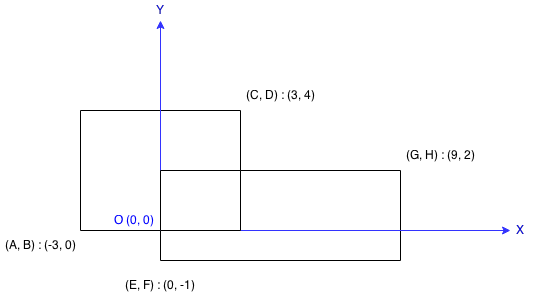
\includegraphics[width=0.8\textwidth]{rectangle-area.png}\\
    \figcaption{Rectangle Area}\label{fig:rectangle-area}
\end{center}

Assume that the total area is never beyond the maximum possible value of \fn{int}.

\subsubsection{分析}
Instead of checking whether the rectangles overlap, I max right with left (and top with bottom). Haven't seen that in other solutions.

\subsubsection{代码}
\begin{Code}
class Solution {
    public:
    int computeArea(int A, int B, int C, int D, int E, int F, int G, int H) {
        int left = max(A,E), right = max(min(C,G), left);
        int bottom = max(B,F), top = max(min(D,H), bottom);
        return (C-A)*(D-B) - (right-left)*(top-bottom) + (G-E)*(H-F);
    }
}
\end{Code}

\subsubsection{分析和代码}
The original version wasn't passing anymore because of new test cases that cause overflow. So now we're avoiding computing the differences below if the result will be negative. This avoids overflow in cases where the rectangles are far apart. It looks like this is basically the same thing that @shw1500 was suggesting, but you don't need the extra max function on the outside.

The return statement is based on comments from @StefanPochmann. We want to avoid forming the sum area(R1) + area(R2). This avoids overflow in cases where area(R1) + area(R2) will overflow, but area(R1) + area(R2) - overlap(R1, R2) fits in an int. There aren't any test cases for this. Add some maybe? Edit: There are test cases for this, but the overflow didn't matter.

New version- avoids overflow when area(R1) + area(R2) overflows but the answer shouldn't.

\begin{Code}
class Solution {
    public:
    int computeArea(int A, int B, int C, int D, int E, int F, int G, int H) {
        int overlap_width = min(C, G) > max(A, E) ? min(C, G) - max(A, E) : 0; 
        int overlap_height = min(D, H) > max(B, F) ? min(D, H) - max(B, F) : 0;
        // order avoids overflow
        return ((C - A) * (D - B) - overlap_width * overlap_height) + (G - E) * (H - F); 
    }
};
\end{Code}

Second version- avoids overflow when rectangles are far apart

\begin{Code}
class Solution {
    public:
    int computeArea(int A, int B, int C, int D, int E, int F, int G, int H) {
        int overlap_width = min(C, G) > max(A, E) ? min(C, G) - max(A, E) : 0; 
        int overlap_height = min(D, H) > max(B, F) ? min(D, H) - max(B, F) : 0;
        return (C - A) * (D - B) + (G - E) * (H - F) - overlap_width * overlap_height;
    }
};
\end{Code}

Old version- overflows for some inputs where the rectangles are far apart.

\begin{Code}
class Solution {
    public:
    int computeArea(int A, int B, int C, int D, int E, int F, int G, int H) {
        int overlap_width = max(min(C, G) - max(A, E), 0);
        int overlap_height = max(min(D, H) - max(B, F), 0);
        return (C - A) * (D - B) + (G - E) * (H - F) - overlap_width * overlap_height;
    }
};
\end{Code}

\subsubsection{相关题目}
\begindot
\item 无
\myenddot

\section{Number of 1 Bits (loj191)} %%%%%%%%%%%%%%%%%%%%%%%%%%%%%%
\label{sec:number-of-1-bits}

\subsubsection{描述}

Write a function that takes an unsigned integer and returns the number of ’1' bits it has (also known as the Hamming weight).

For example, the 32-bit integer ’11' has binary representation \fn{00000000000000000000000000001011}, so the function should return 3.

\subsubsection{分析}

n \& (n - 1) drops the lowest set bit. It's a neat little bit trick.

Let's use n = 00101100 as an example. This binary representation has three 1s.

If n = 00101100, then n - 1 = 00101011, so n \& (n - 1) = 00101100 \& 00101011 = 00101000. Count = 1.

If n = 00101000, then n - 1 = 00100111, so n \& (n - 1) = 00101000 \& 00100111 = 00100000. Count = 2.

If n = 00100000, then n - 1 = 00011111, so n \& (n - 1) = 00100000 \& 00011111 = 00000000. Count = 3.

n is now zero, so the while loop ends, and the final count (the numbers of set bits) is returned.

\subsubsection{代码}
\begin{Code}
class Solution {
public:
    int hammingWeight(uint32_t n) {
        int count = 0;
        while (n) {
            n &= (n - 1);
            count++;
        }
        return count;
    }
};
\end{Code}

\subsubsection{代码}
\begin{Code}
class Solution {
public:
    int hammingWeight(uint32_t n) {
        int sum=0;
        while(n) {
            if(n % 2 == 1) sum++;
            n /= 2; 
        }
        return sum;
    }
};
\end{Code}

\subsubsection{相关题目}

\begindot
\item 无
\myenddot

\appendix % 开始附录,章用字母编号
\printindex

\end{document}
